\chapter{Appendix}
\label{sec:appendix}
\section{$\wpr$ Search}
\subsection{CA8 b-tagging}
\label{sec:ca8toak5}
%The Full statistics QCD MC closure test can be seen in figure \ref{figs:QCDClosure1}.  Here there is an excess of full selection over background at high $M_{\tbbar}$.  
%The kinematic bias is not manifest in the current data selection.

%\begin{figure}[Htcb]
%\begin{center}
%\subfigure{\label{figs:MtbvsBkgQCDEOfullstats}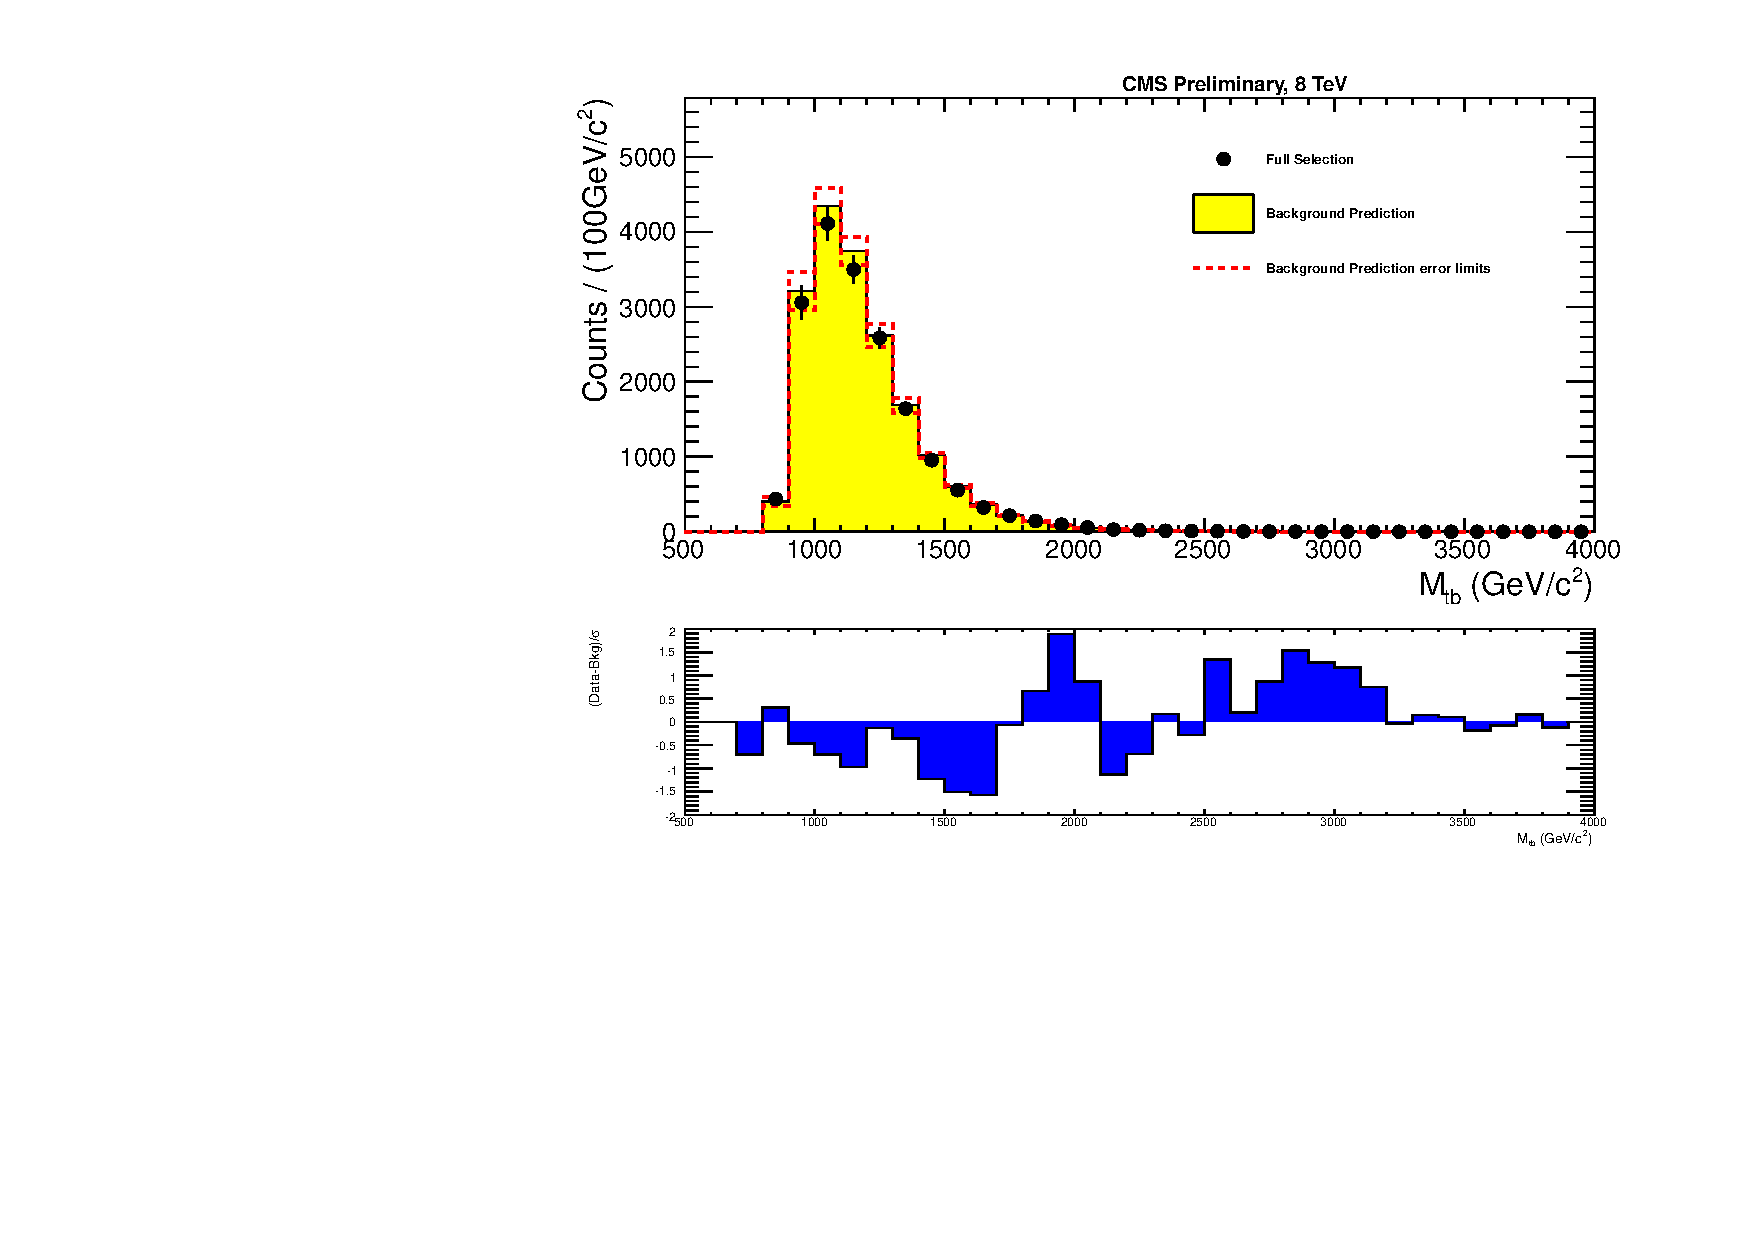
\includegraphics[width=1.0\textwidth]{figs/MtbvsBkgQCDEOfullstats.pdf}}\\
%\subfigure{\label{figs:MtbvsBkgsemilog_QCDEOfullstats}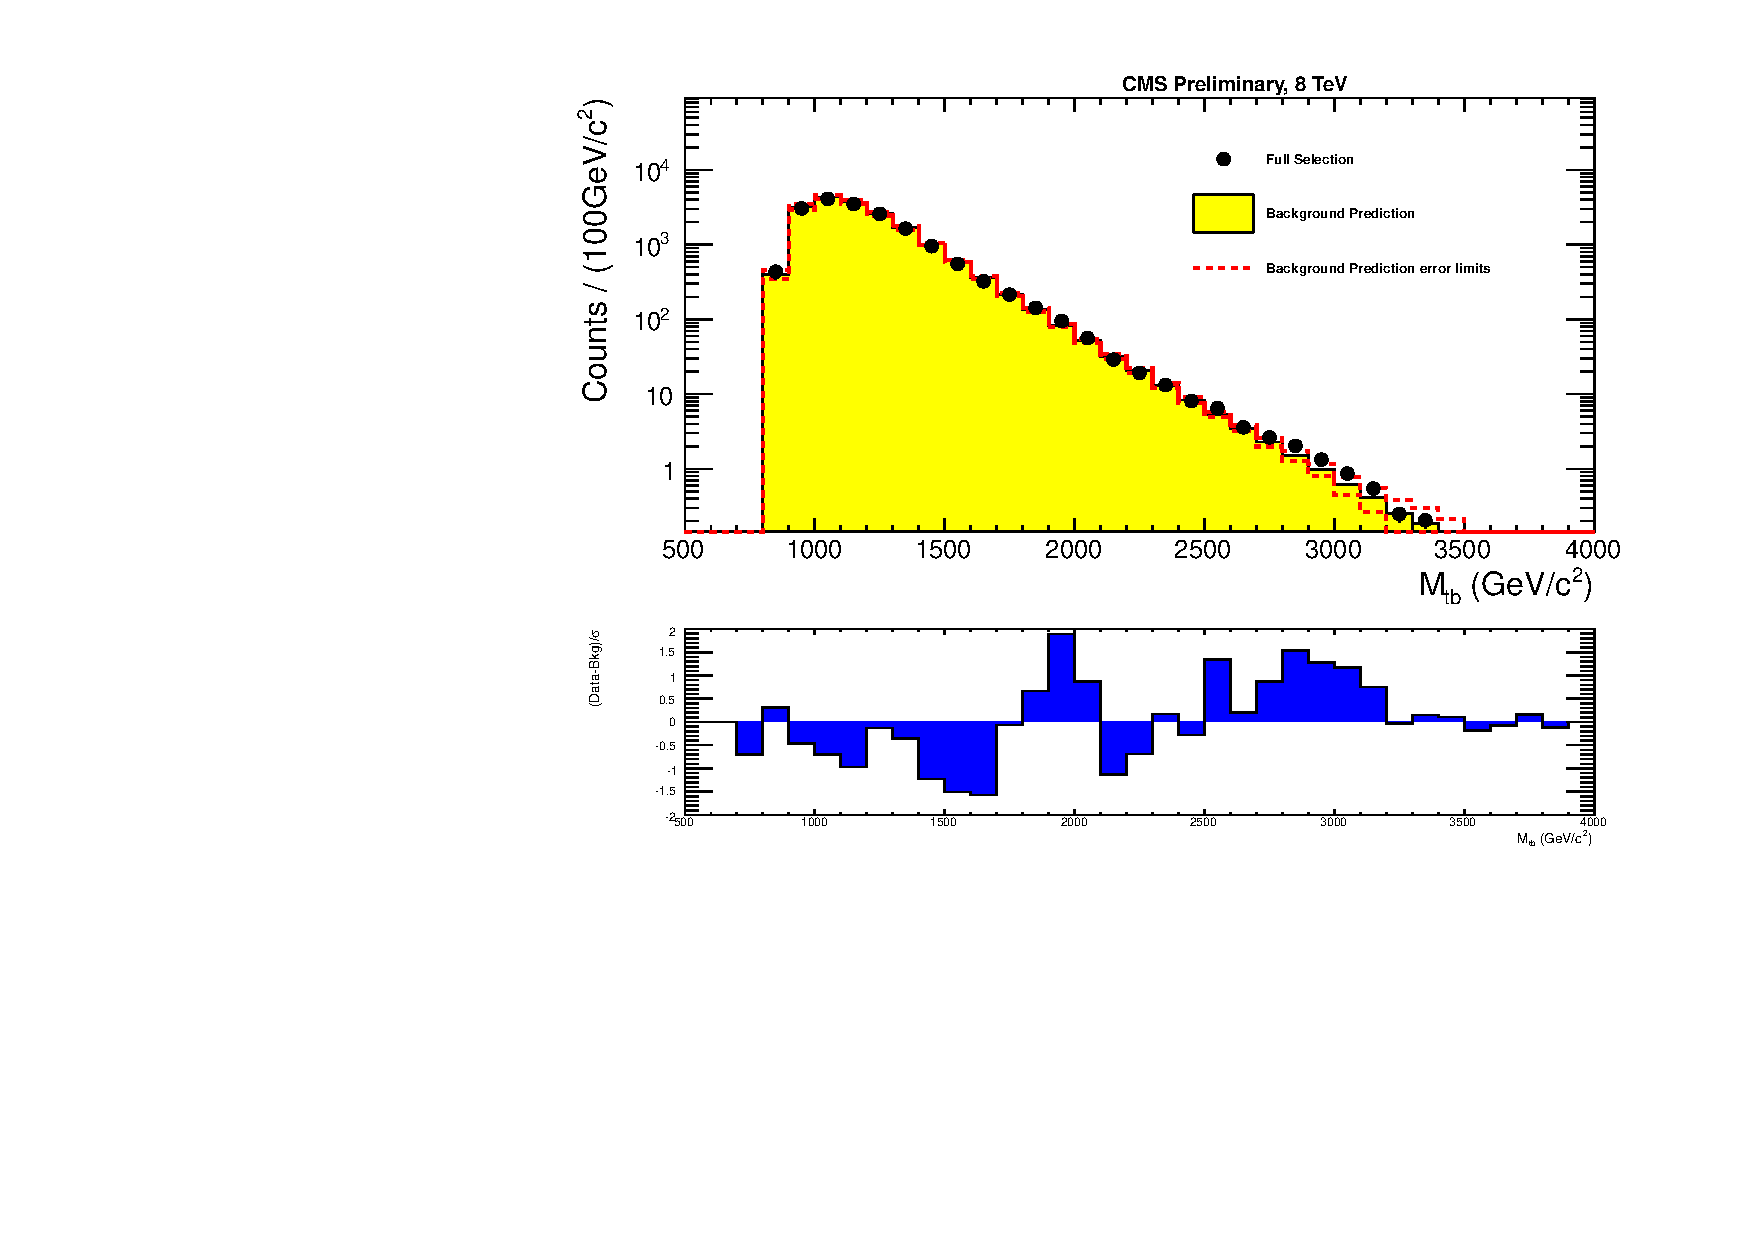
\includegraphics[width=1.0\textwidth]{figs/MtbvsBkgsemilog_QCDEOfullstats.pdf}}
%\caption{
%QCD MC background estimation closure test.  The full selection is shown in black, 
%the background estimation is shown in yellow, and the errors from the background estimation are shown as a red dashed line.}
%\label{figs:QCDClosure1}
%\end{center}
%\end{figure}

CA8 jet b-tagging comparison to AK5 jets. A 2\% uncertainty is applied to signal MC samples in the analysis.  Jets are matched between AK5 and CA8 
within a Delta(R) size of 0.3.
Jets are ensured b flavor from MC truth and are within the pt range of the analysis.  The constant fit to the efficiency ratio gives an upper limit to the uncertainty 
for the change in $SF_b$ for use with CA8 jets.  No extra correction is applied to $SF_b$.  The following plots are from Signal MC at 2700$/GeV$. 
%Efficiency Ratio comparison in ttbar MC can be seen in figure \ref{figs:EfficiencyCompr5ttbar}.  

\begin{figure}[Htcb]
\centering
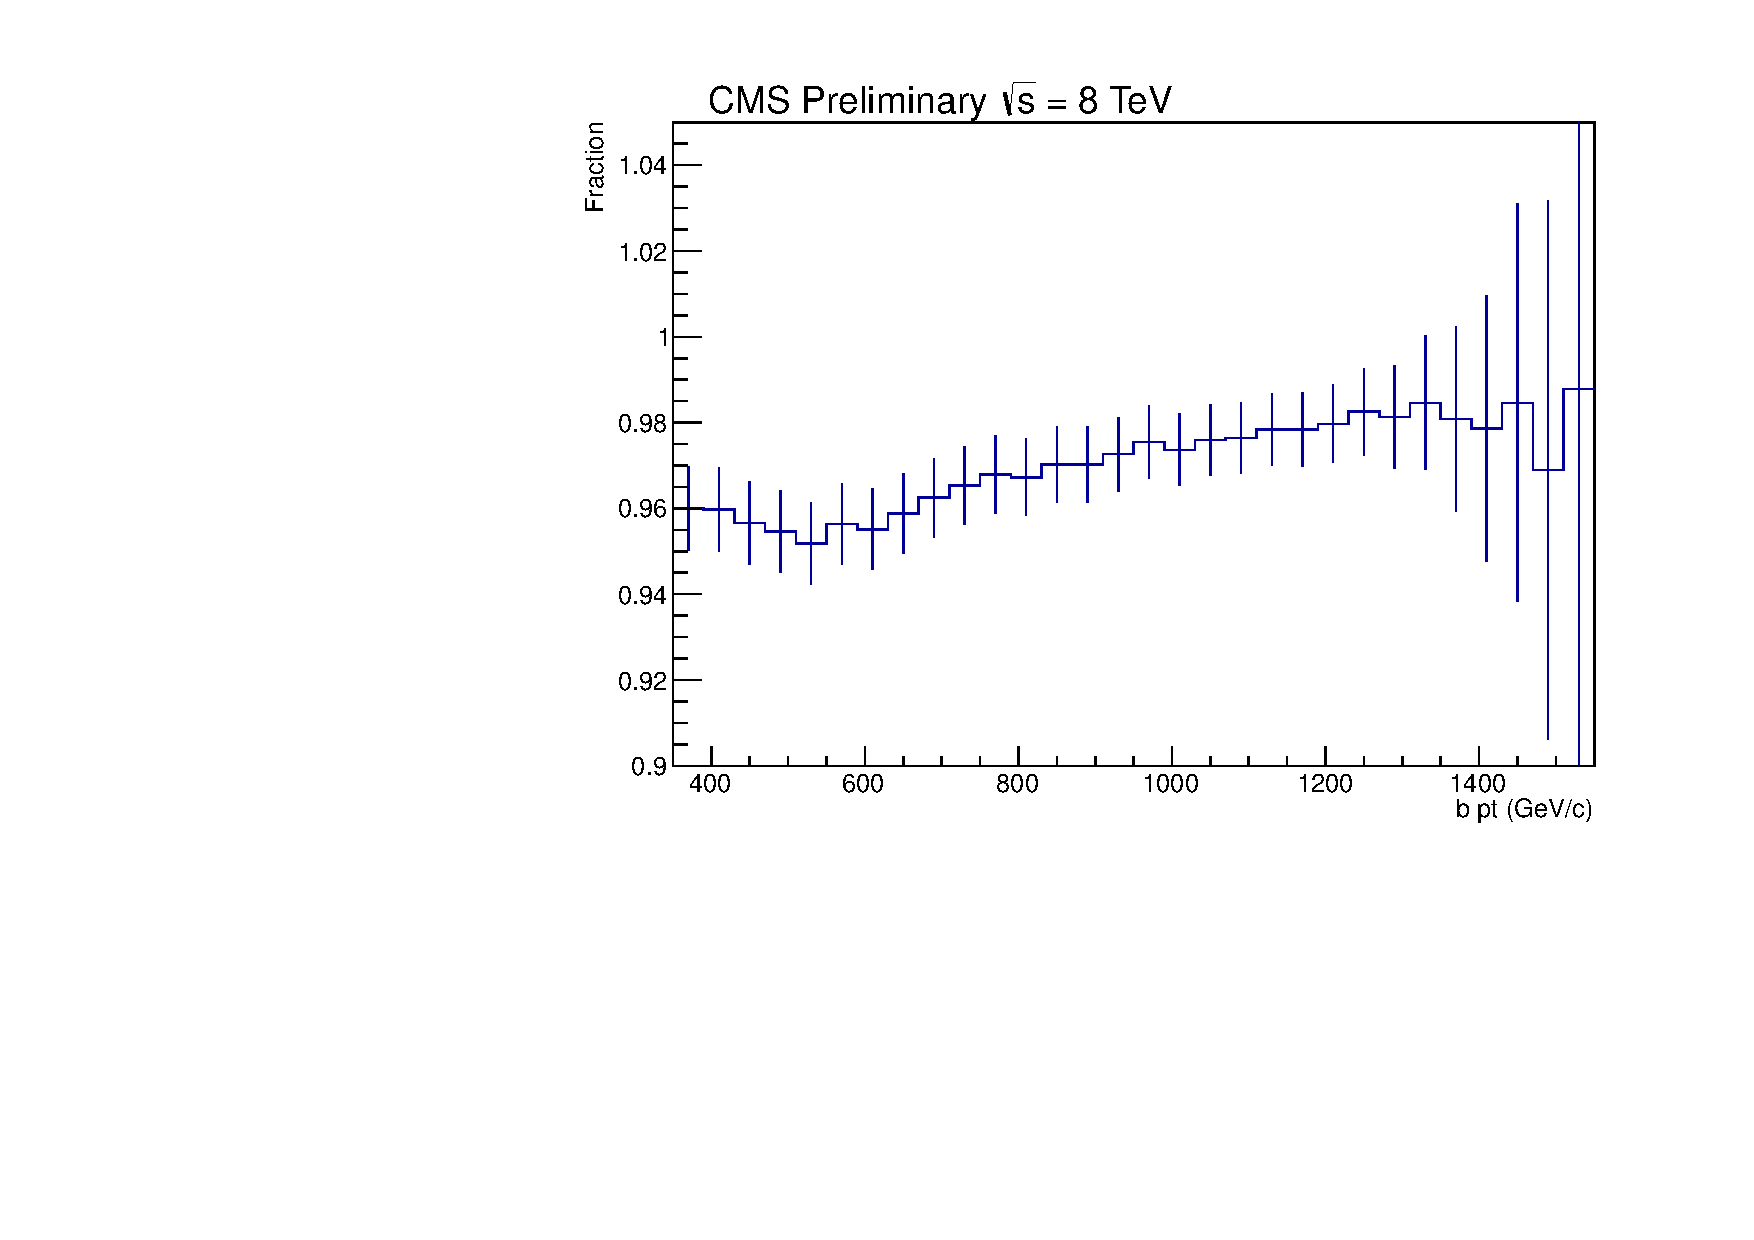
\includegraphics[width=1.0\textwidth]{figs/bpercentr32700.pdf}
\caption{Percent of matched jets that register the same value for the CSVM cut.}
\label{figs:bpercent}
\end{figure}

\begin{figure}[Htcb]
\centering
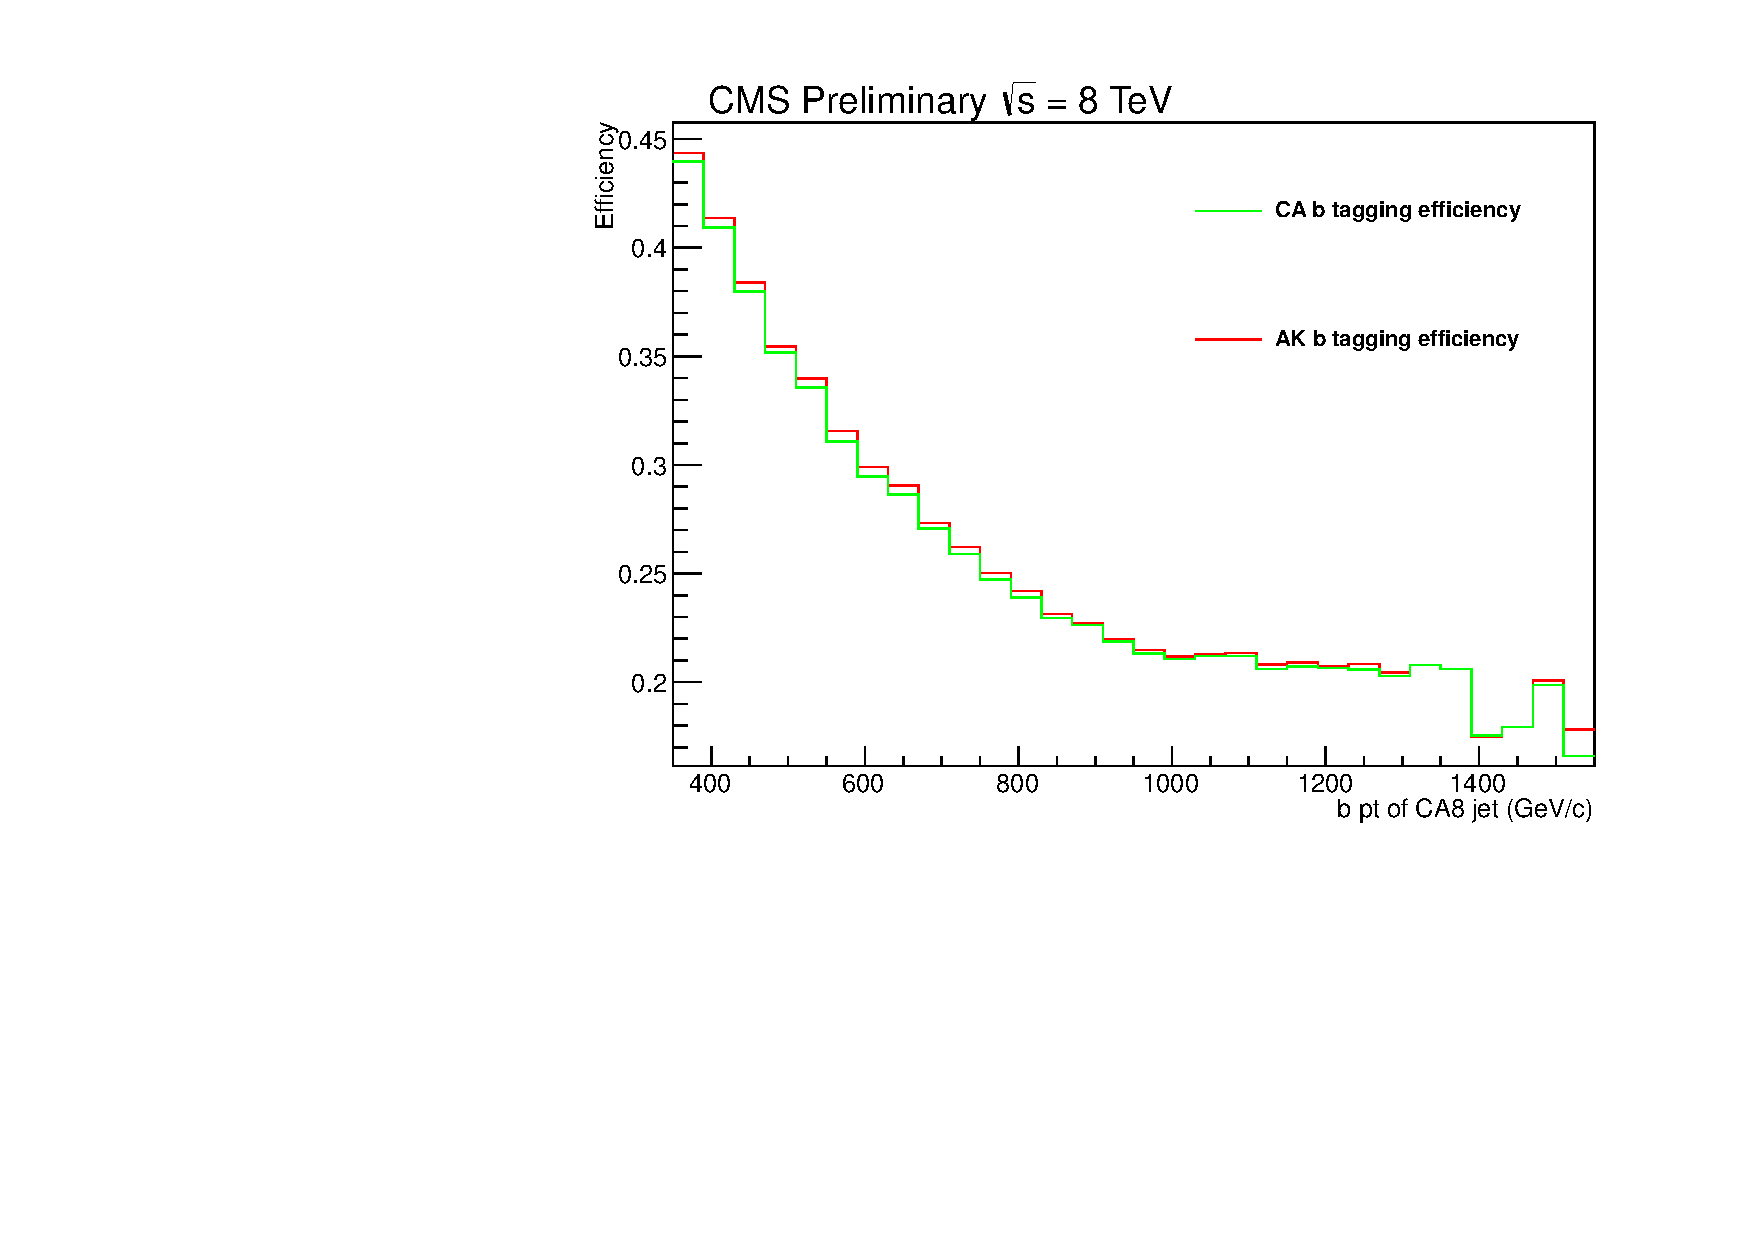
\includegraphics[width=1.0\textwidth]{figs/beffCAptr32700.pdf}
\caption{Comparison of the efficiency of b-tagging matched CA8 and AK5 jets}
\label{figs:beff}
\end{figure}

%\begin{figure}[Htcb]
%\centering
%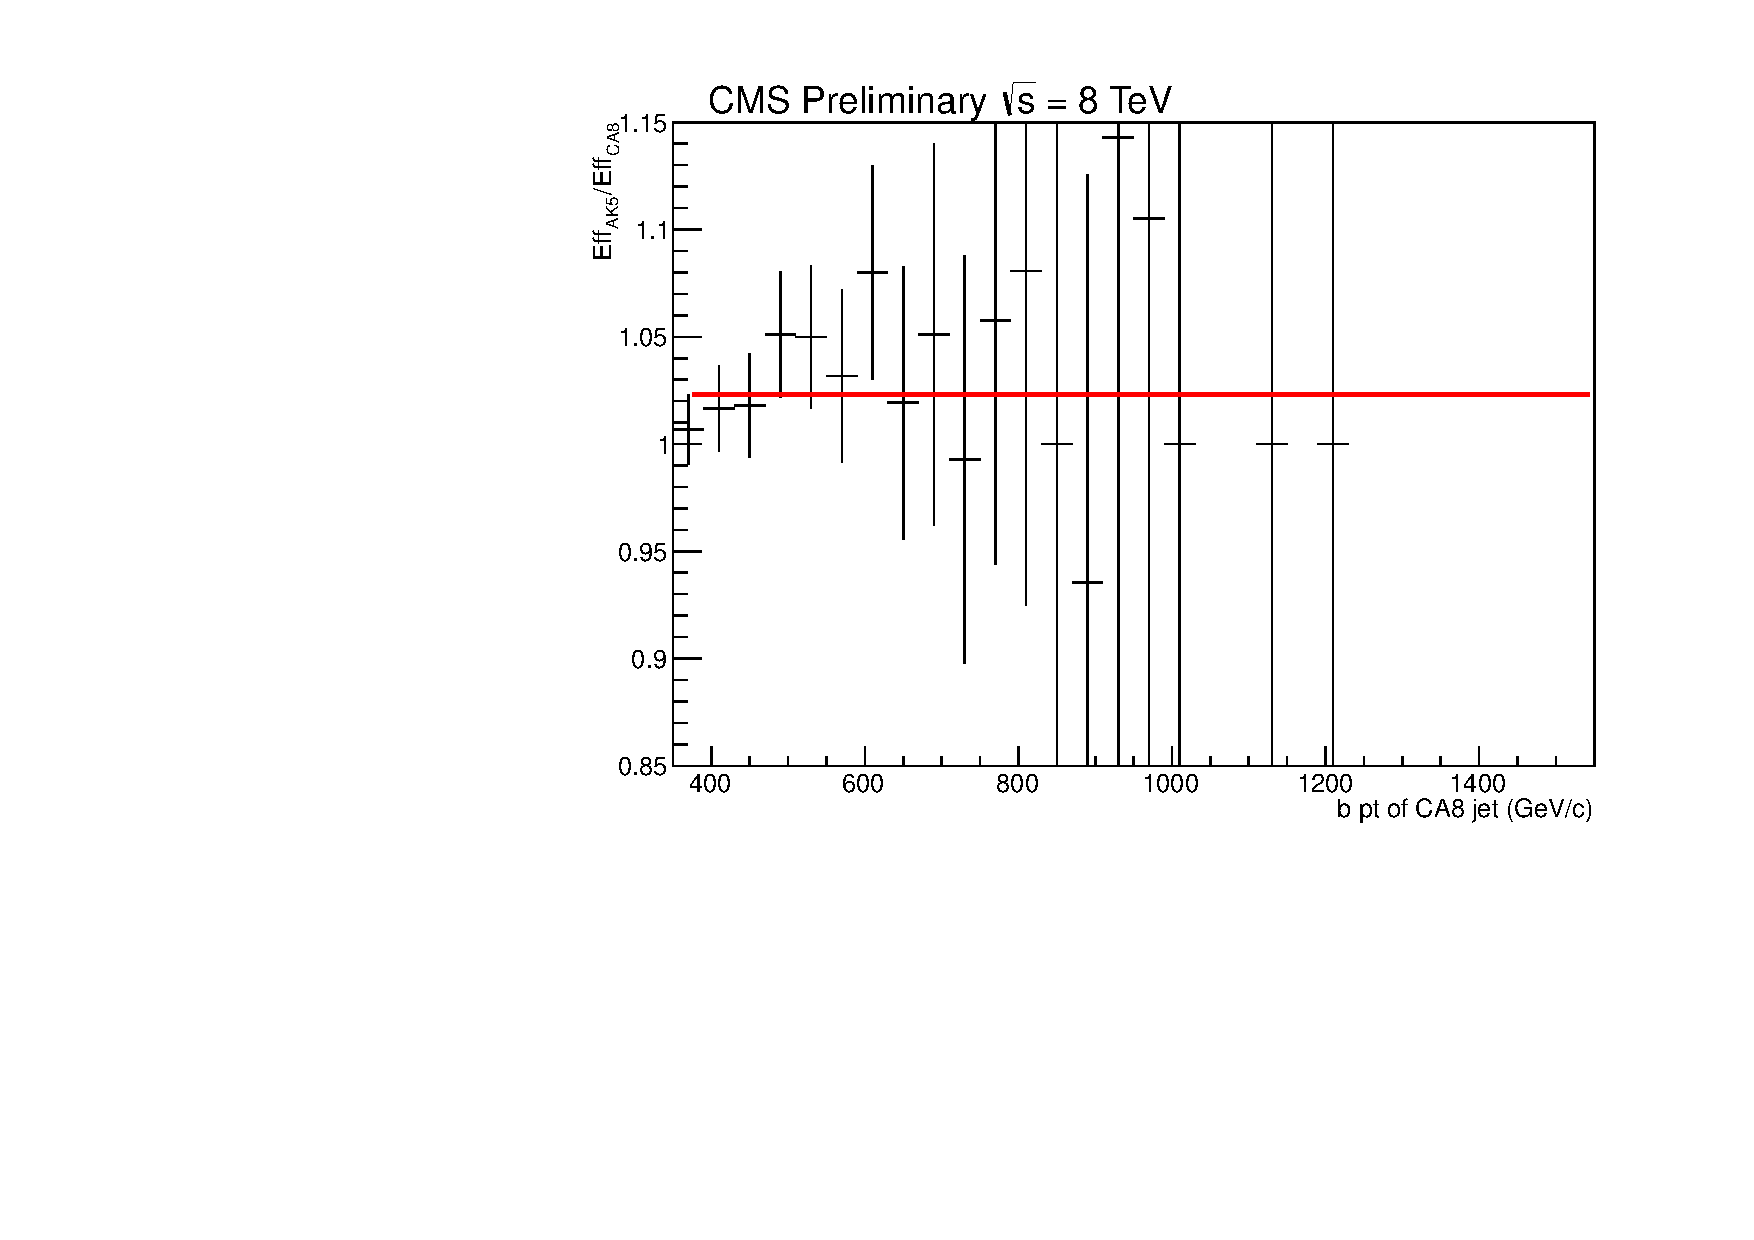
\includegraphics[width=1.0\textwidth]{figs/EfficiencyCompCAptr3none.pdf}
%\caption{Comparison of the ratio of efficiency of b-tagging matched CA8 and AK5 jets in ttbar MC.  The fit here is 1.023}
%\label{figs:EfficiencyCompr5ttbar}
%\end{figure}


%Fit comparison of the tagrates as extracted from the sideband and signal region Can be seen in Figure \ref{figs:tagrateetafitQCD_withSR}.  
%This comparison was extracted from QCD MC.
%\begin{figure}[Htcb]
%\begin{center}
%\subfigure{\label{figs:tagrateeta1fitQCD_withSR}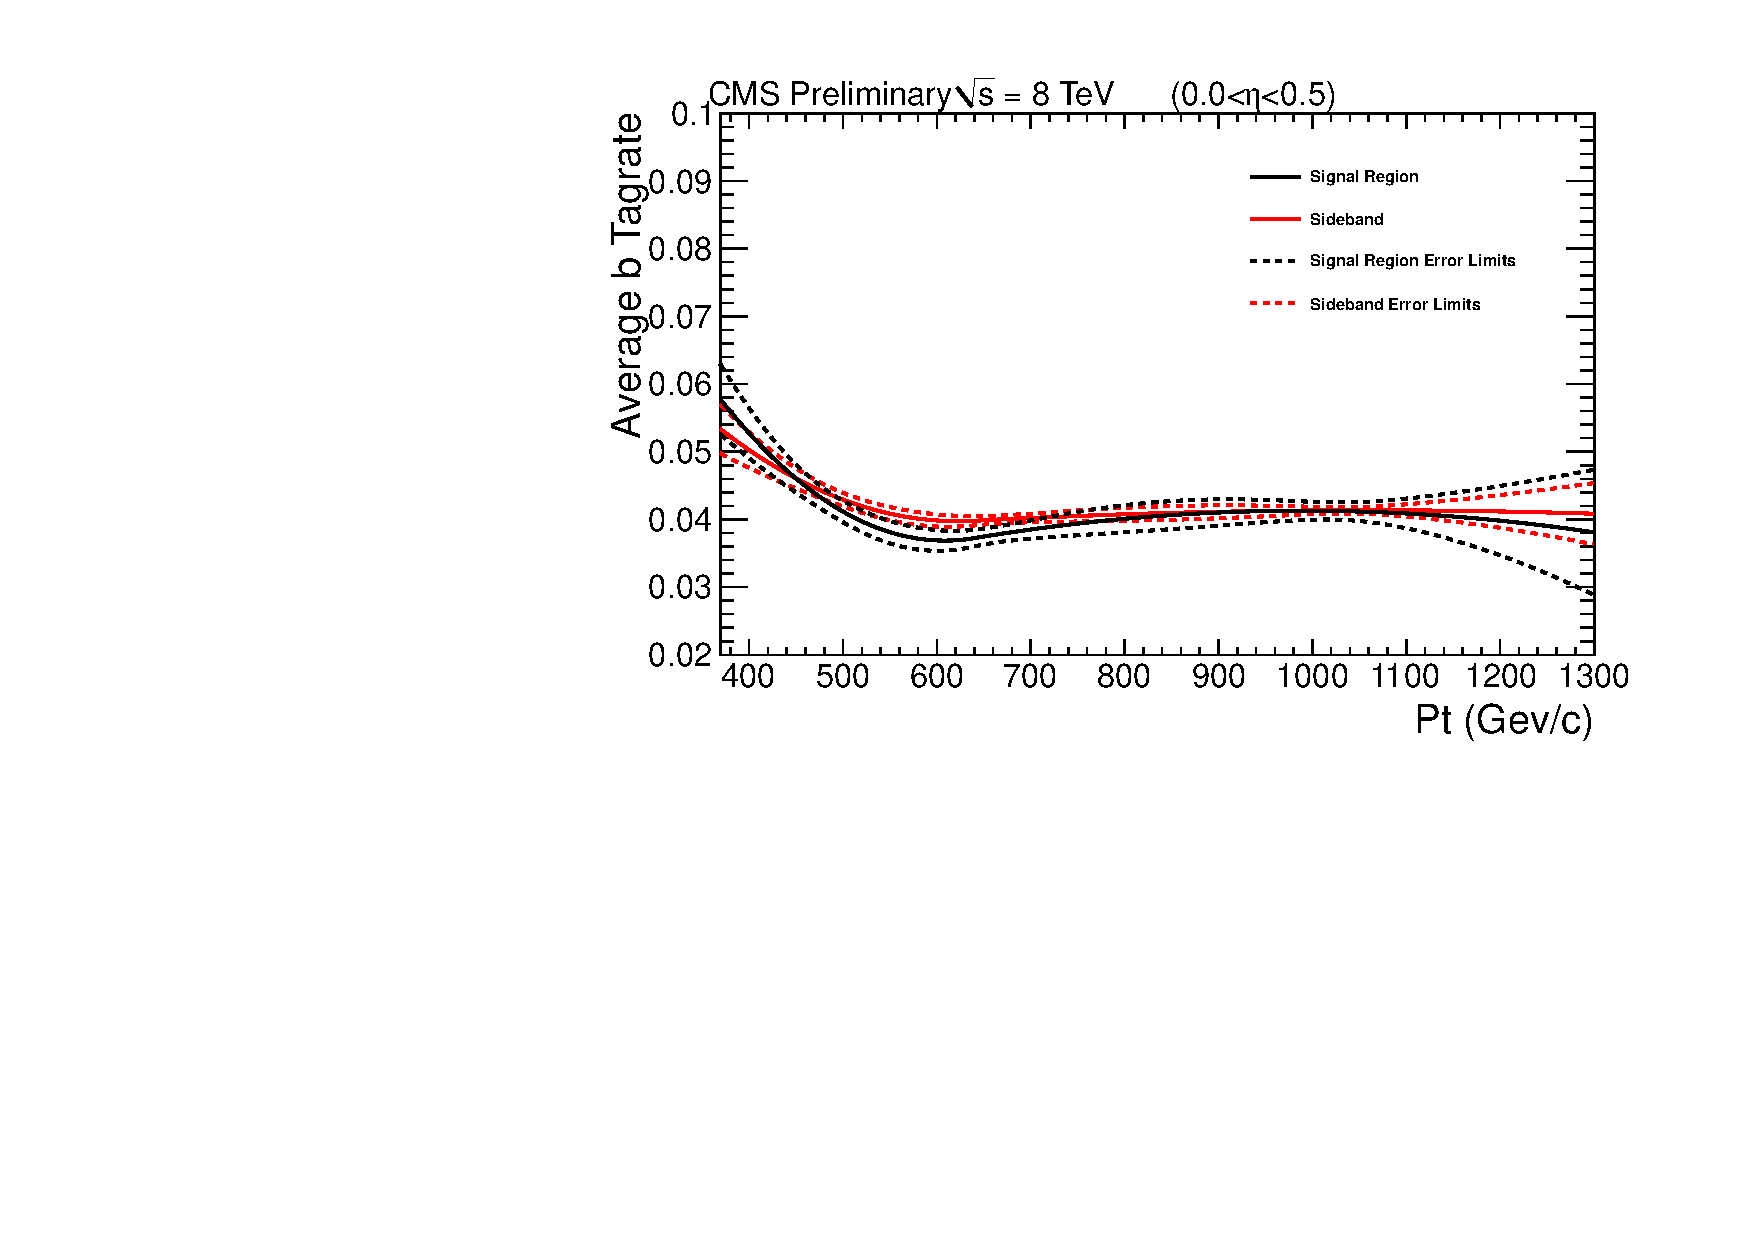
\includegraphics[width=0.75\textwidth]{figs/tagrateeta1fitQCD_withSR}}\\
%\subfigure{\label{figs:tagrateeta2fitQCD_withSR}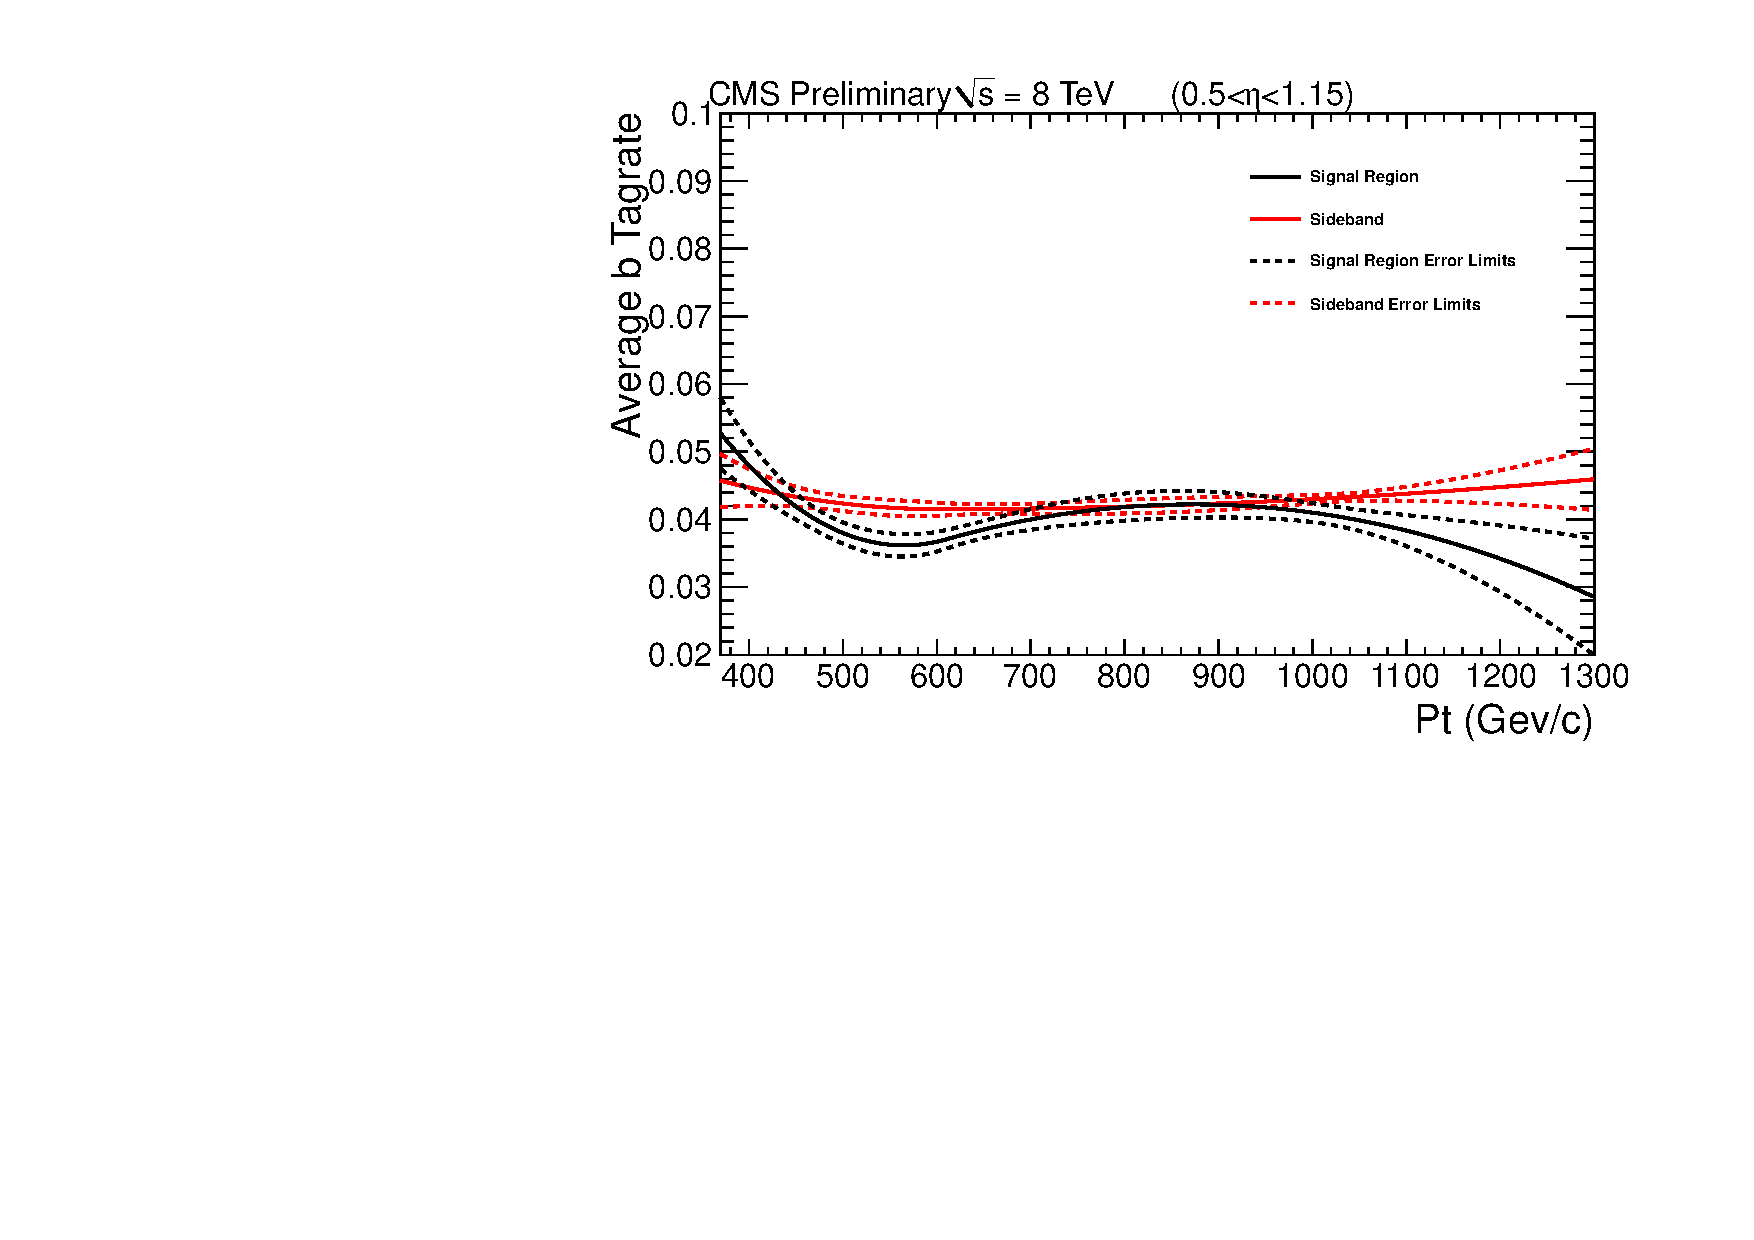
\includegraphics[width=0.75\textwidth]{figs/tagrateeta2fitQCD_withSR}}\\
%\subfigure{\label{figs:tagrateeta3fitQCD_withSR}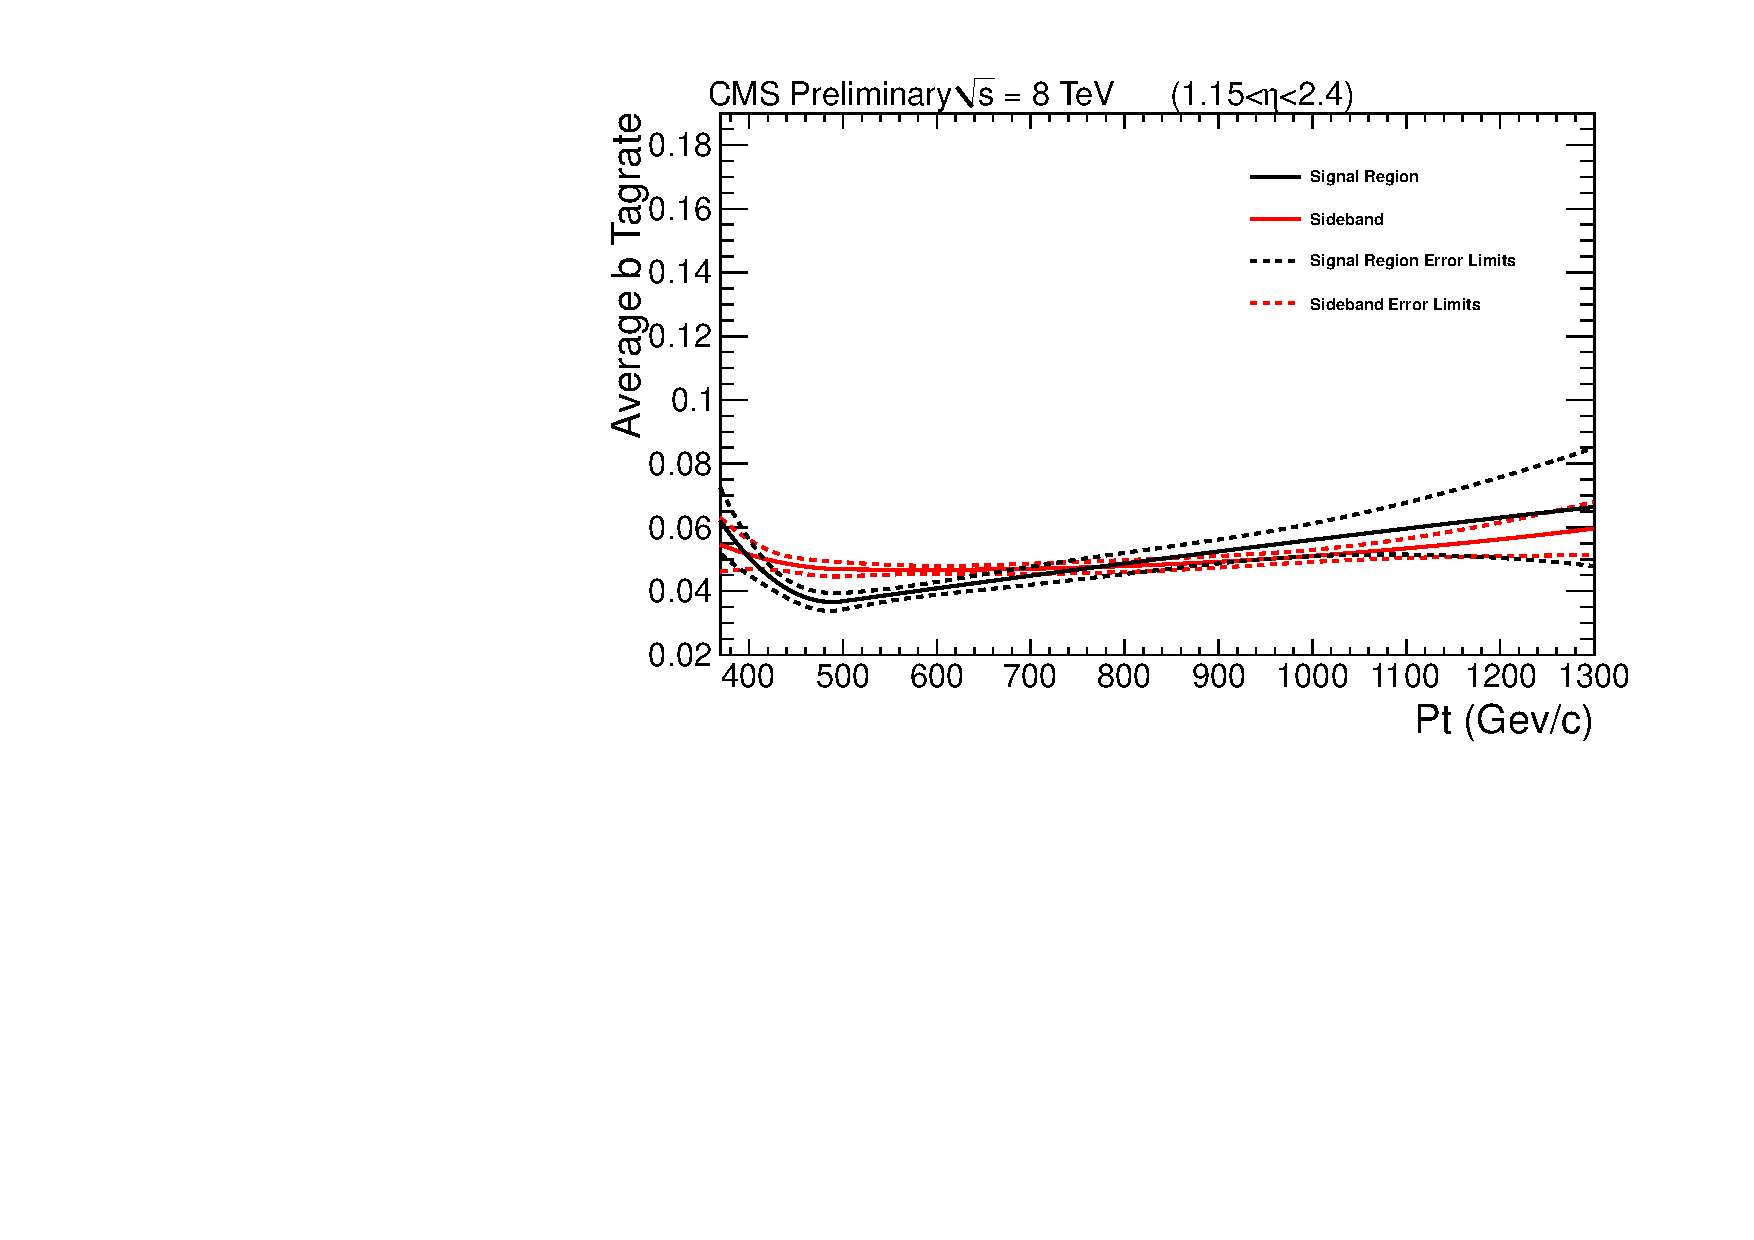
\includegraphics[width=0.75\textwidth]{figs/tagrateeta3fitQCD_withSR}}
%\caption{
%QCD MC $\pt$ parameterized tagrate fit comparison to the signal region from
%(a) Low $\eta$ region  
%(b) Transition $\eta$ region 
%(c) High $\eta$ region 
%the fit from the Signal Region is shown in black, the fit from the Sideband is shown in red.}
%\label{figs:tagrateetafitQCD_withSR}
%\end{center}
%\end{figure}



\subsection{Signal Region and Sideband Kinematic Comparison}
\label{sec:SBvsSR}
Figure \ref{figs:SBtoSR} shows a comparison in QCD MC of kinematic variables of interest in the CMS top tagger selection and number of subjets sideband used for the determination of the average b-tagging rate.  There are some discrepancies 
seen in the two regions, which is the main reason why we use the average b-tagging rate instead of the sideband itself.  Variables constrained to the top candidate jet such as top mass have a drastically different shape, so we need to look at the 
b candidate jet in the opposite hemisphere to keep the background estimate unbiased.  Additionally, because we parameterize in $\pt$ the influence from the different b candidate $\pt$ shapes does not bias the background estimate.  Then the final 
kinematic variable of interest is b candidate mass which shows good agreement.  


\begin{figure}[Htcb]
\centering
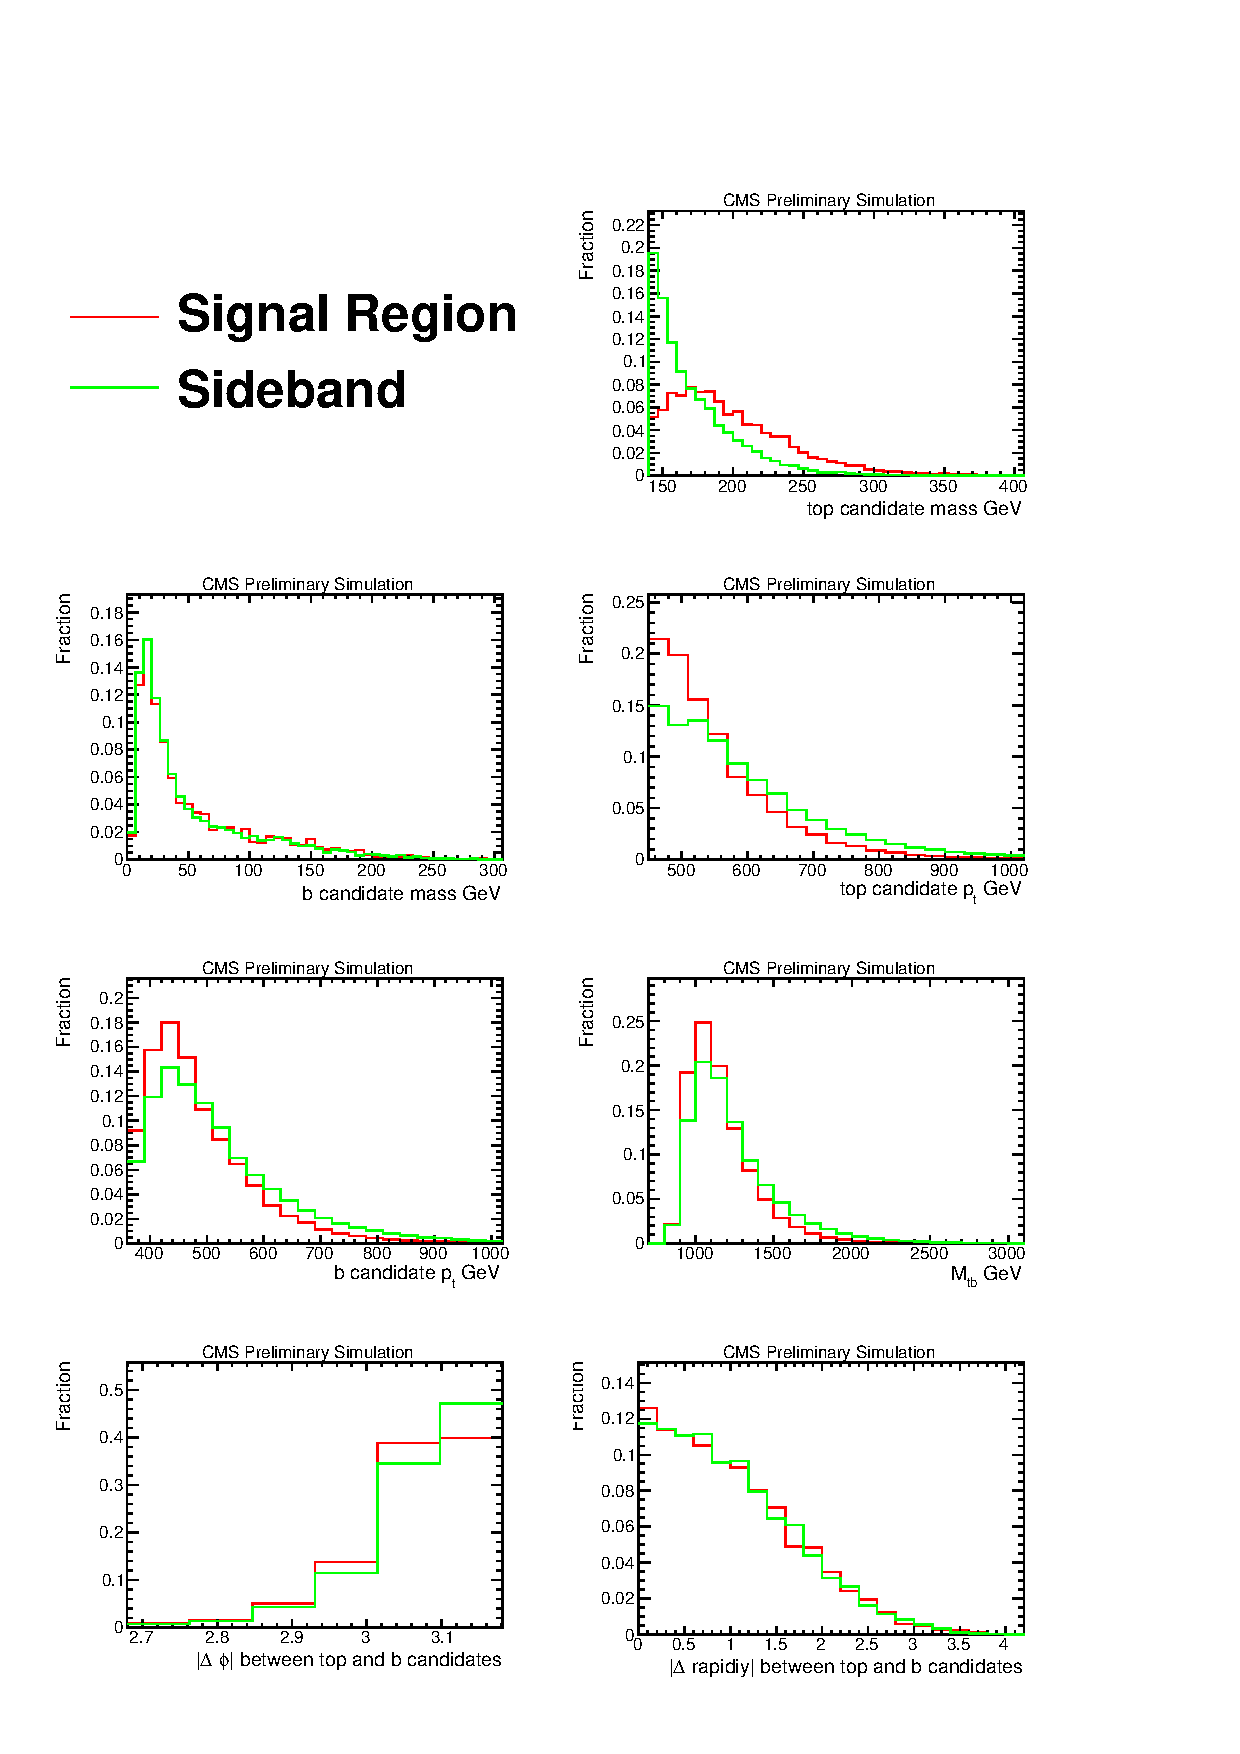
\includegraphics[width=0.8\textwidth]{figs/SBtoSR.pdf}
\caption{Comparison of kinematic variables in QCD MC extracted from the CMS top tagger signal region and number of subjets sideband}
\label{figs:SBtoSR}
\end{figure}



\subsection{Signal Kinematic Comparison}
\label{sec:SigKinGen}
Figure \ref{figs:genkin} shows a comparison of relevant kinematic variables for right, left, and mixed Signal MC samples.


\begin{figure}[Htcb]
\centering
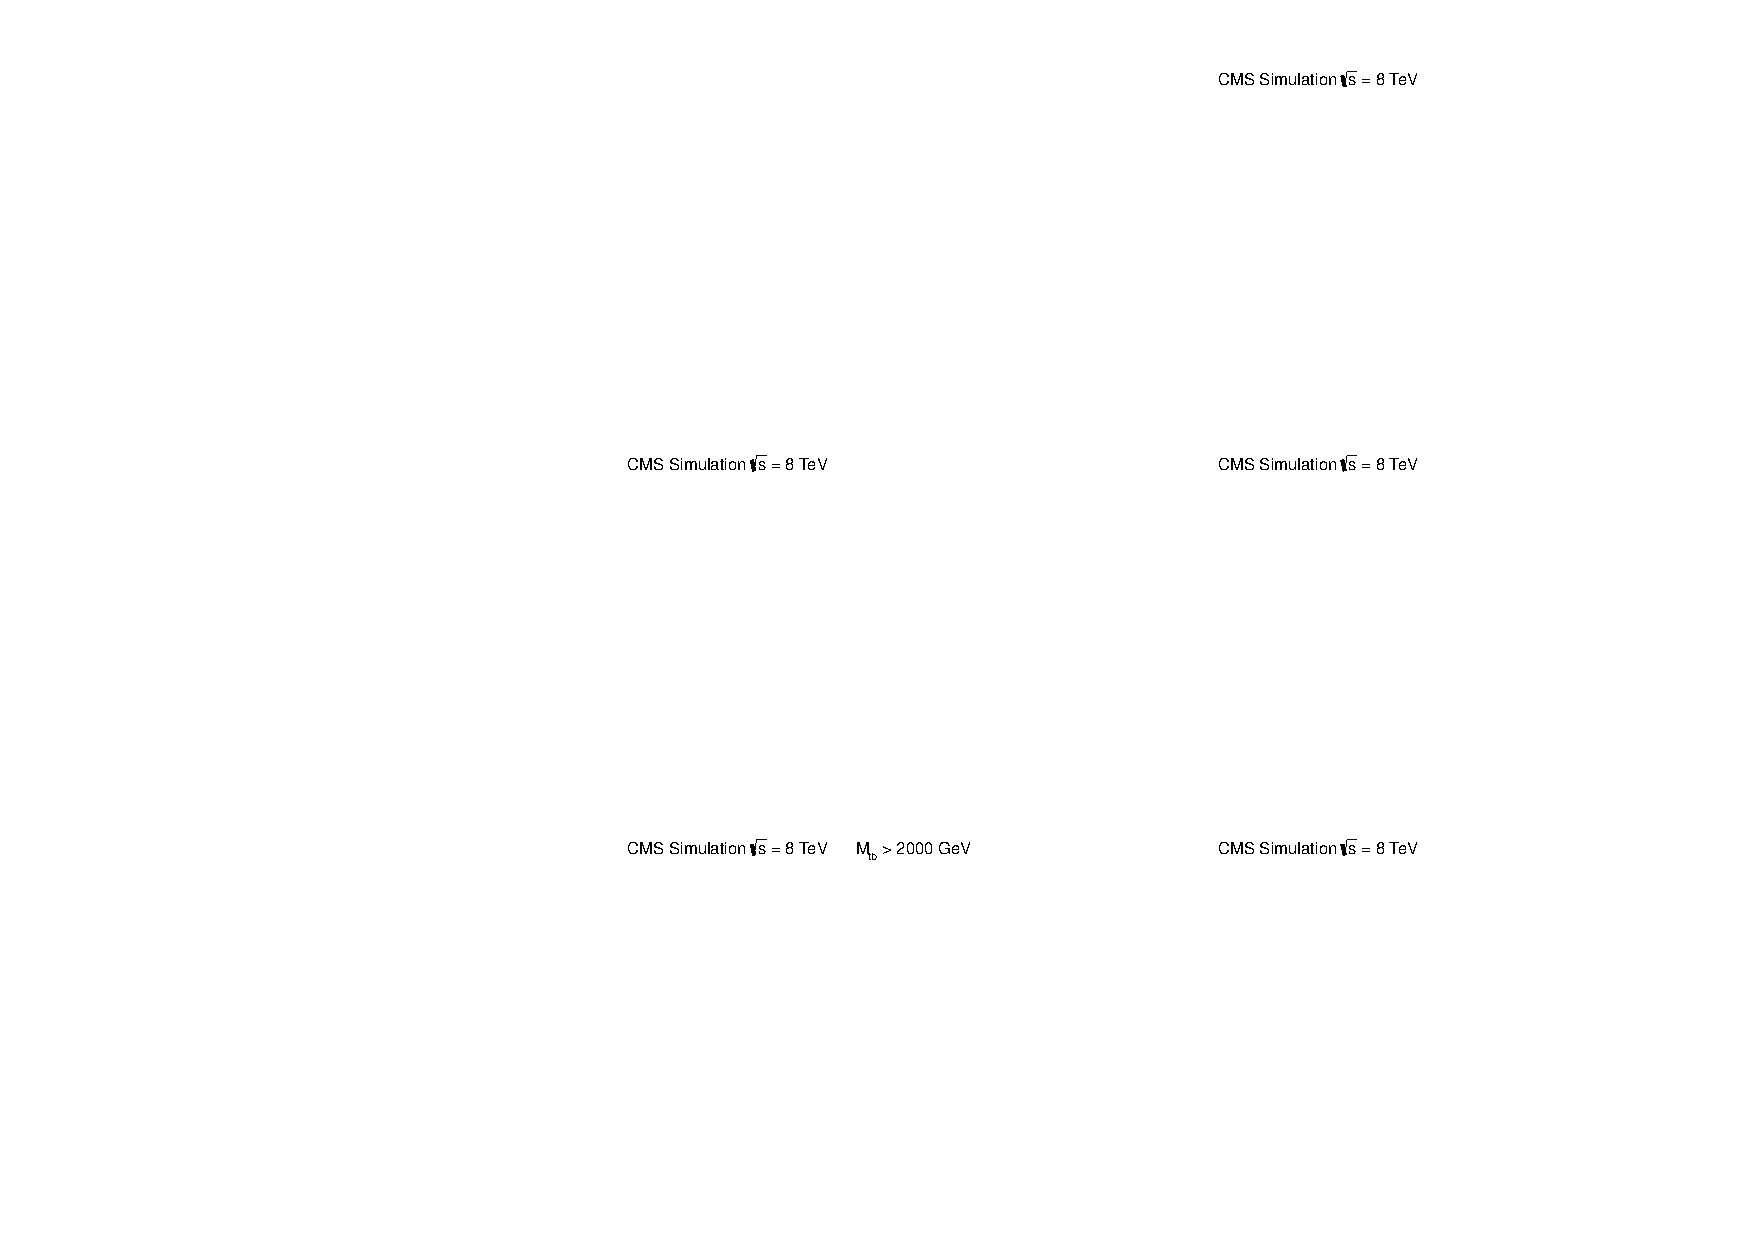
\includegraphics[width=1.0\textwidth]{figs/CutCompqcdandsignalGencoupling.pdf}
\caption{Comparison of kinematic variables in Signal MC for right, left and mixed coupling all at the 2100$~\GeV$ mass point }
\label{figs:genkin}
\end{figure}



%\clearpage

%\section{Top Pt Re-weighting}
%\label{sec:tptrw}
%One possible improvement for the QCD background estimate relies on weighting the top pt.  The method is to weight events such that the pt of the 
%top jet in full selection is equal to the background estimate.  In this implementation, the weight is obtained from QCD MC and applied to data.
%The weight can be seen in figure \ref{figs:QCDWeight}.  Applying this weight to the data full selection results in 
%figure \ref{figs:tptweightedmtb}.  In QCD closure test for this procedure, the weight is extracted from even 
%events in the QCD MC and applied to odd events.  The resulting $M_{tb}$ plot is shown in figure \ref{figs:tptweightedmtbQCD}.

%We also investigate the effect of this correction in the second sideband seen in figure \ref{figs:NewMtbSB2}.  Using the top pt weight as 
%extracted from QCD MC in this selection produces the $M_{tb}$ plot seen in figure \ref{figs:tptweightedmtbSB2}. % The limits extracted from this procedure are shown in figure \ref{figs:limits_theta_comb_log_tptweight}.

%\begin{figure}[Htcb]
%\centering
%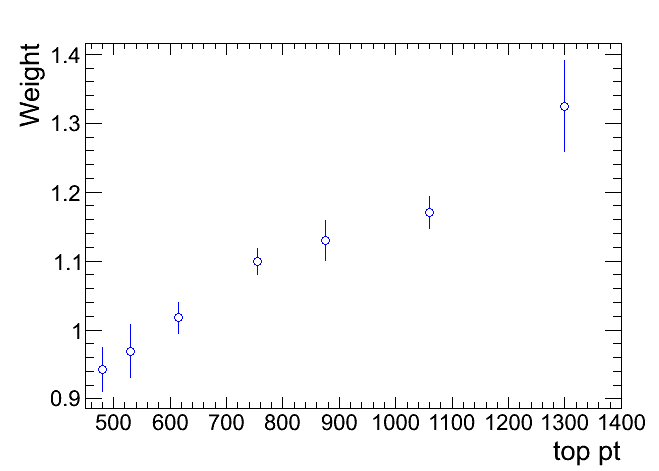
\includegraphics[width=1.0\textwidth]{figs/tptweightplotfromQCD.png}
%\caption{Top pt weight as extracted from QCD MC.}
%\label{figs:QCDWeight}
%\end{figure}

%\begin{figure}[Htcb]
%\centering
%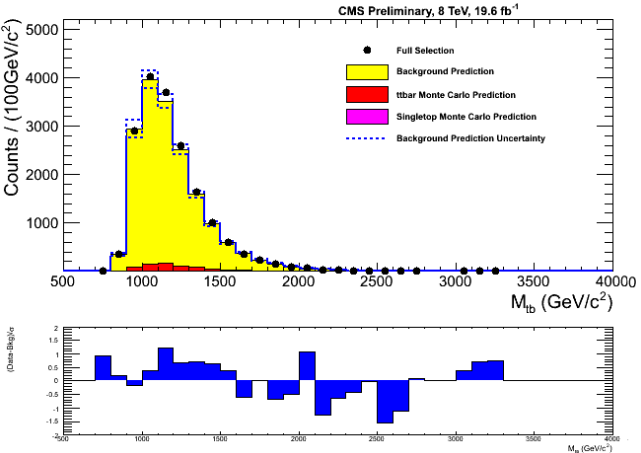
\includegraphics[width=1.0\textwidth]{figs/tptweightedmtb.png}
%\caption{Top pt weighted full selection in the data full selection.}
%\label{figs:tptweightedmtb}
%\end{figure}

%\begin{figure}[Htcb]
%\centering
%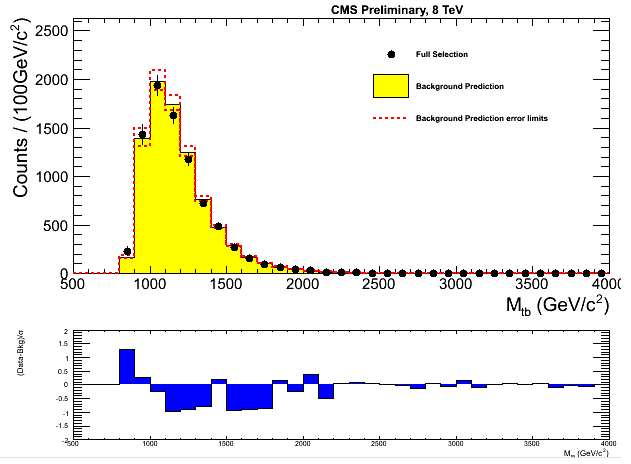
\includegraphics[width=1.0\textwidth]{figs/tptweightedmtbQCD.png}
%\caption{Top pt weighted QCD closure test.}
%\label{figs:tptweightedmtbQCD}
%\end{figure}



%\begin{figure}[Htcb]
%\centering
%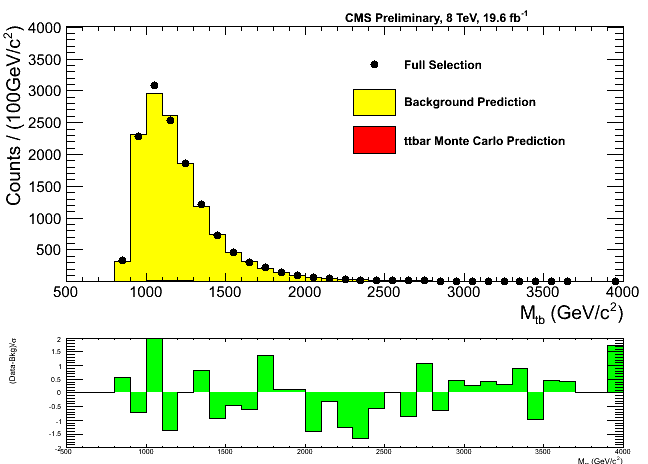
\includegraphics[width=1.0\textwidth]{figs/tptweightedmtbSB2.png}
%\caption{Control region $M_{tb}$ plot with top pt weighting.  As of this version of the note, systematics on this sample have not been computed.  
%The sigma referenced in the lower green plot is just statistical.}
%\label{figs:tptweightedmtbSB2}
%\end{figure}

%\begin{figure}[Htcb]
%\centering
%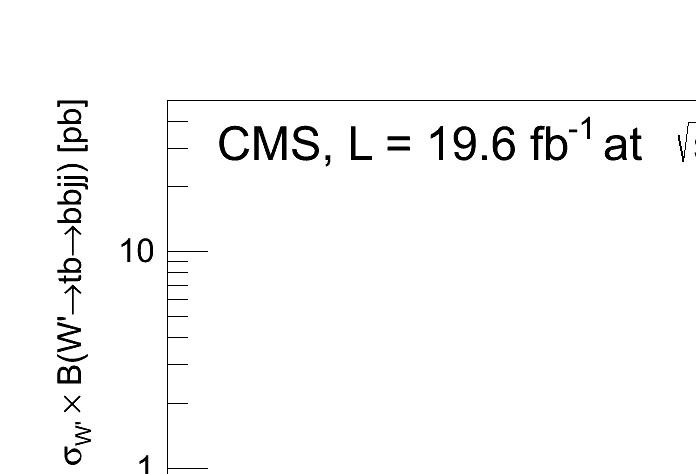
\includegraphics[width=1.0\textwidth]{figs/limits_theta_comb_log_tptweight.png}
%\caption{Limits extracted by using the top pt weighting procedure}
%\label{figs:limits_theta_comb_log_tptweight}
%\end{figure}

\clearpage

\subsection{QCD Parameterization Uncertainty}
\label{sec:qcdpunc}

The QCD background prediction relies on the probability to tag a b~jet.  
We parameterize this probability using physical variables that
have a large effect on the b-tagging rate ($\pt$ and $\eta$ of the b
candidate jet).  However, the variable of interest in the analysis
is $M_{tb}$, and the background estimate involves integrating, for
every bin in $M_{tb}$, along the $\pt$ axis.  To see this more
explicitly, let us consider the signal region only, with pre-b-tag
data divided into a two-dimensional matrix along $\pt$ and
$M_{tb}$ axes, indexed by indices $i$ and $j$ respectively.
Thus $n_{ij}$ is the number of pre-b-tag events within a given $\pt$
bin (index $i$) and a given $M_{tb}$ bin (index $j$), 
$\overline P_i$ is the average of true b-tagging probability for a slice 
in $\pt$, whereas $P_{ij}$ is the true b-tagging probability for
data in $n_{ij}$.

The true number of b tags in two-dimensional bin $(i,j)$ is then
$n_{ij} P_{ij}$.  The observed number of events in $M_{tb}$ bin $j$ is
$N_j = \sum_i n_{ij} P_{ij}$.  However, the background
estimate uses the average b-tagging probability, $\overline P_i$,
averaged over all values of $j$ -- that is, over all values of 
$M_{tb}$.\footnote{In the real measurement we
furthermore obtain this number from the sideband, but to elucidate the
point it is sufficient to consider the average of true b-tagging
probabilities, $P_{ij}$, from the signal region.} 
So a `perfect' background estimate (using probabilities from the
signal region) therefore
yields $N_j^{\rm bkg.est.} = \sum_i n_{ij} \overline P_i$.

Our procedure for the estimation of the QCD background {\it assumes}
that $P_{ij}$ is independent of $M_{tb}$ -- in other words, that
$P_{ij} = \overline P_i$.  If that is the case, the bias of the
background estimate
\begin{equation}
  \delta N_j = N_j - N_j^{\rm bkg.est.} = \sum_i n_{ij} (P_{ij} - \overline P_i)
  \label{eq:qcd_bias}
\end{equation}
is indeed zero.

If for some reason $P_{ij} \neq \overline P_i$, 
Eq.(\ref{eq:qcd_bias}), depending on the values of $n_{ij}$, could
result in non-zero bias $\delta N_j$ -- even when the used 
average tagging probability
corresponds to the signal region itself.

Luckily, the assumption that the average b-tagging probability
depends only on the jet itself (with $\pt$ and $\eta$ of the b~jet)
is a very good one.  However, it is conceivable that second- or
third-order effects could create small deviations in 
$P_{ij} - \overline P_i$ and thus result in a small bias.
These effects could be caused by other activity in the event,
which could be a reason that the same values of $\pt$ and $\eta$ 
could correspond to events with different $\pt$ of the top jet,
and thus $M_{tb}$. To see that such effects exist (and also that
they are small), it is sufficient to consider the top $\pt$ in
Figure \ref{figs:kinplotsdata1}, where there seems to be a small but systematic bias of
the background estimate, as evidenced by the pull distribution
in the lower pane.  We have not studied the causes of these
effects, but additional activity in the event (from other
jets or pile-up) could contribute additional pixel and
strip hits inside the volume of the b jet, and thus impact
the average tagging rate at a low level.

To investigate the ability of the b-tagging rate parameterization in
$\pt$ and $\eta$ to predict $M_{tb}$, we incorporate $M_{tb}$ into the
b-tagging rate parameterization,  The effect is first checked in the
second sideband described above.  The three-dimensional b-tagging rate
shown in Figure \ref{figs:sb2deta} is compared to the two dimensional
tagging rate shown in \ref{figs:tagrateetafit} to see if this effect
can be the cause of the deviations observed in the low $M_{tb}$
region.  Figure \ref{figs:sb2comp} shows the differences in the three
and two dimensional background estimates as well as the differences in
the full selection of this control region and the background estimate.
From this we conclude that there is an effect and the shape of the
deviations is well approximated with this method.

\begin{figure}[Htcb]
\begin{center}
\subfigure{\label{figs:SB2sdBkgMinusBkg}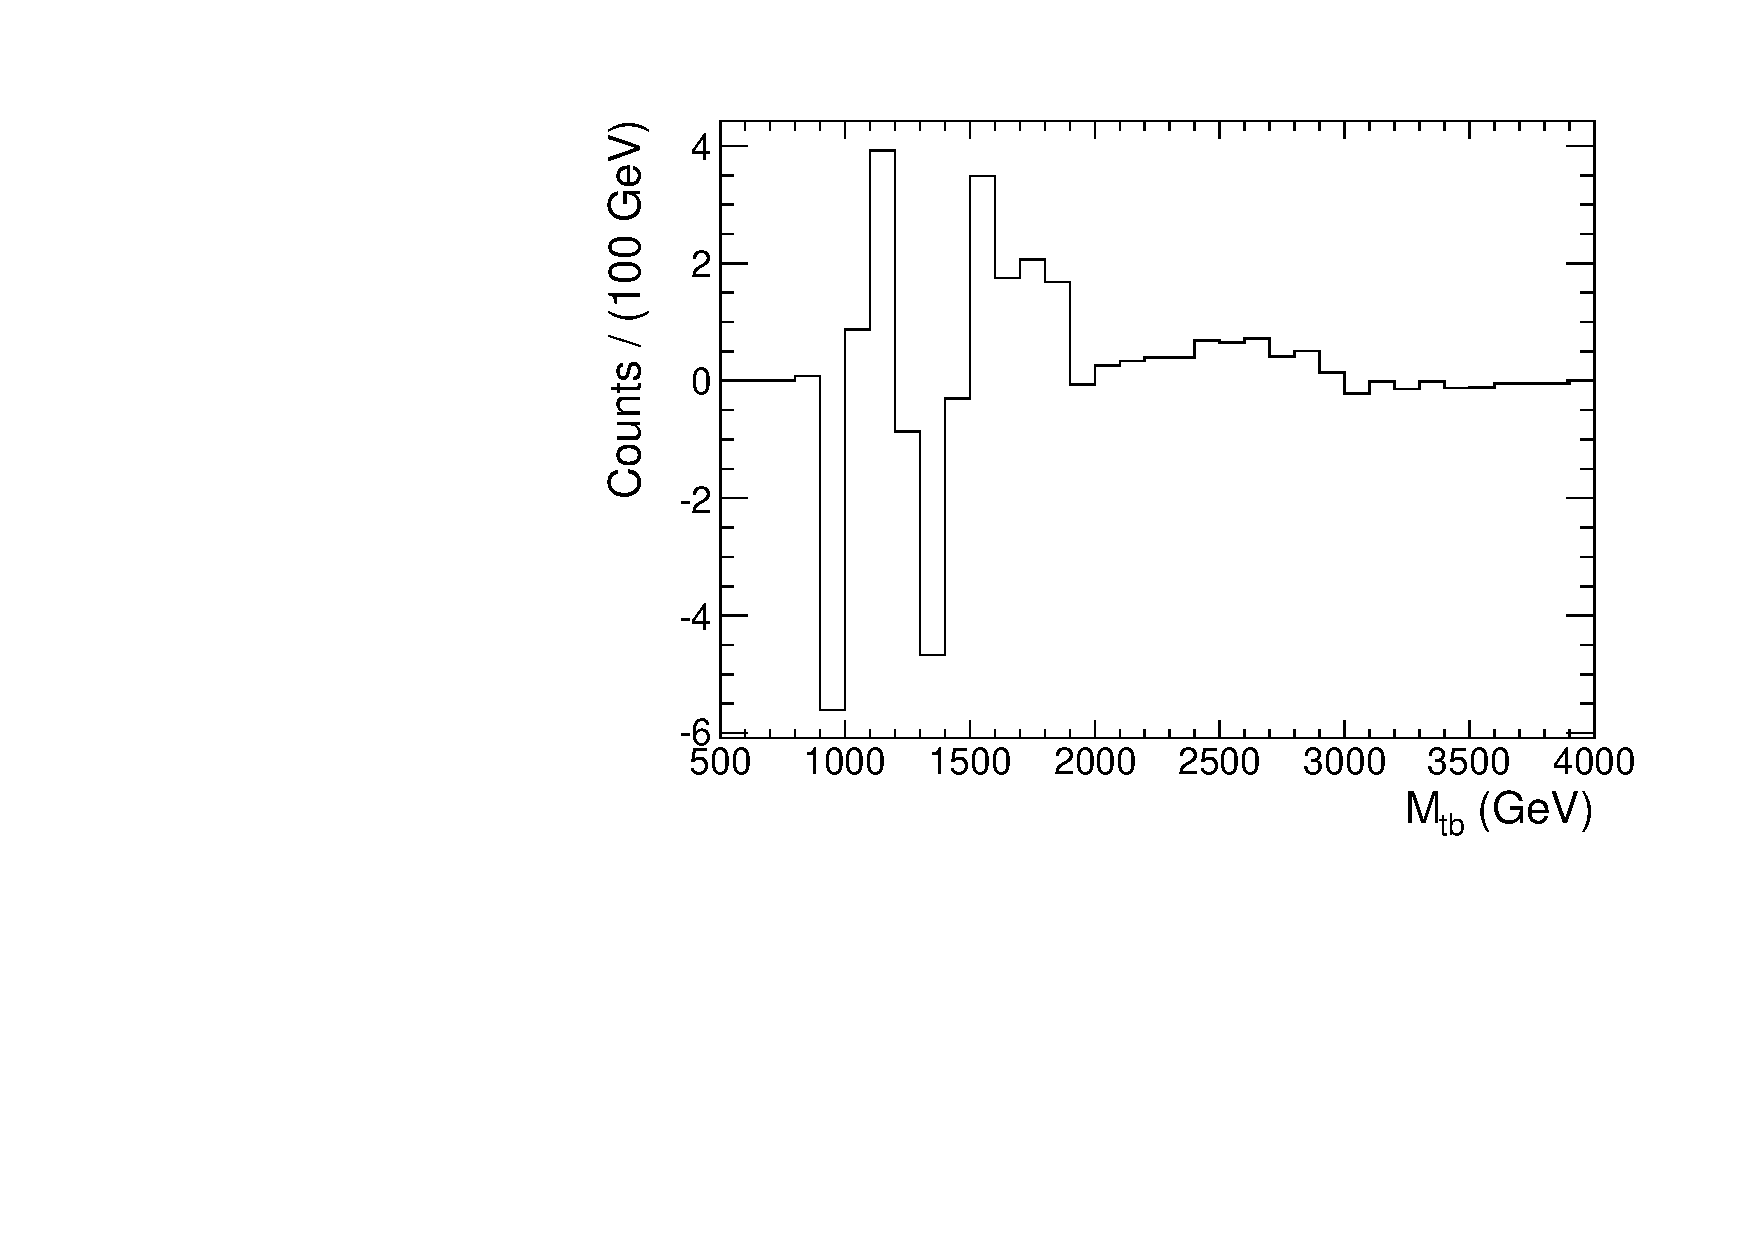
\includegraphics[width=1.0\textwidth]{figs/Mtb2dminus1dBE.pdf}}\\
\subfigure{\label{figs:SB2SRMinusBkg}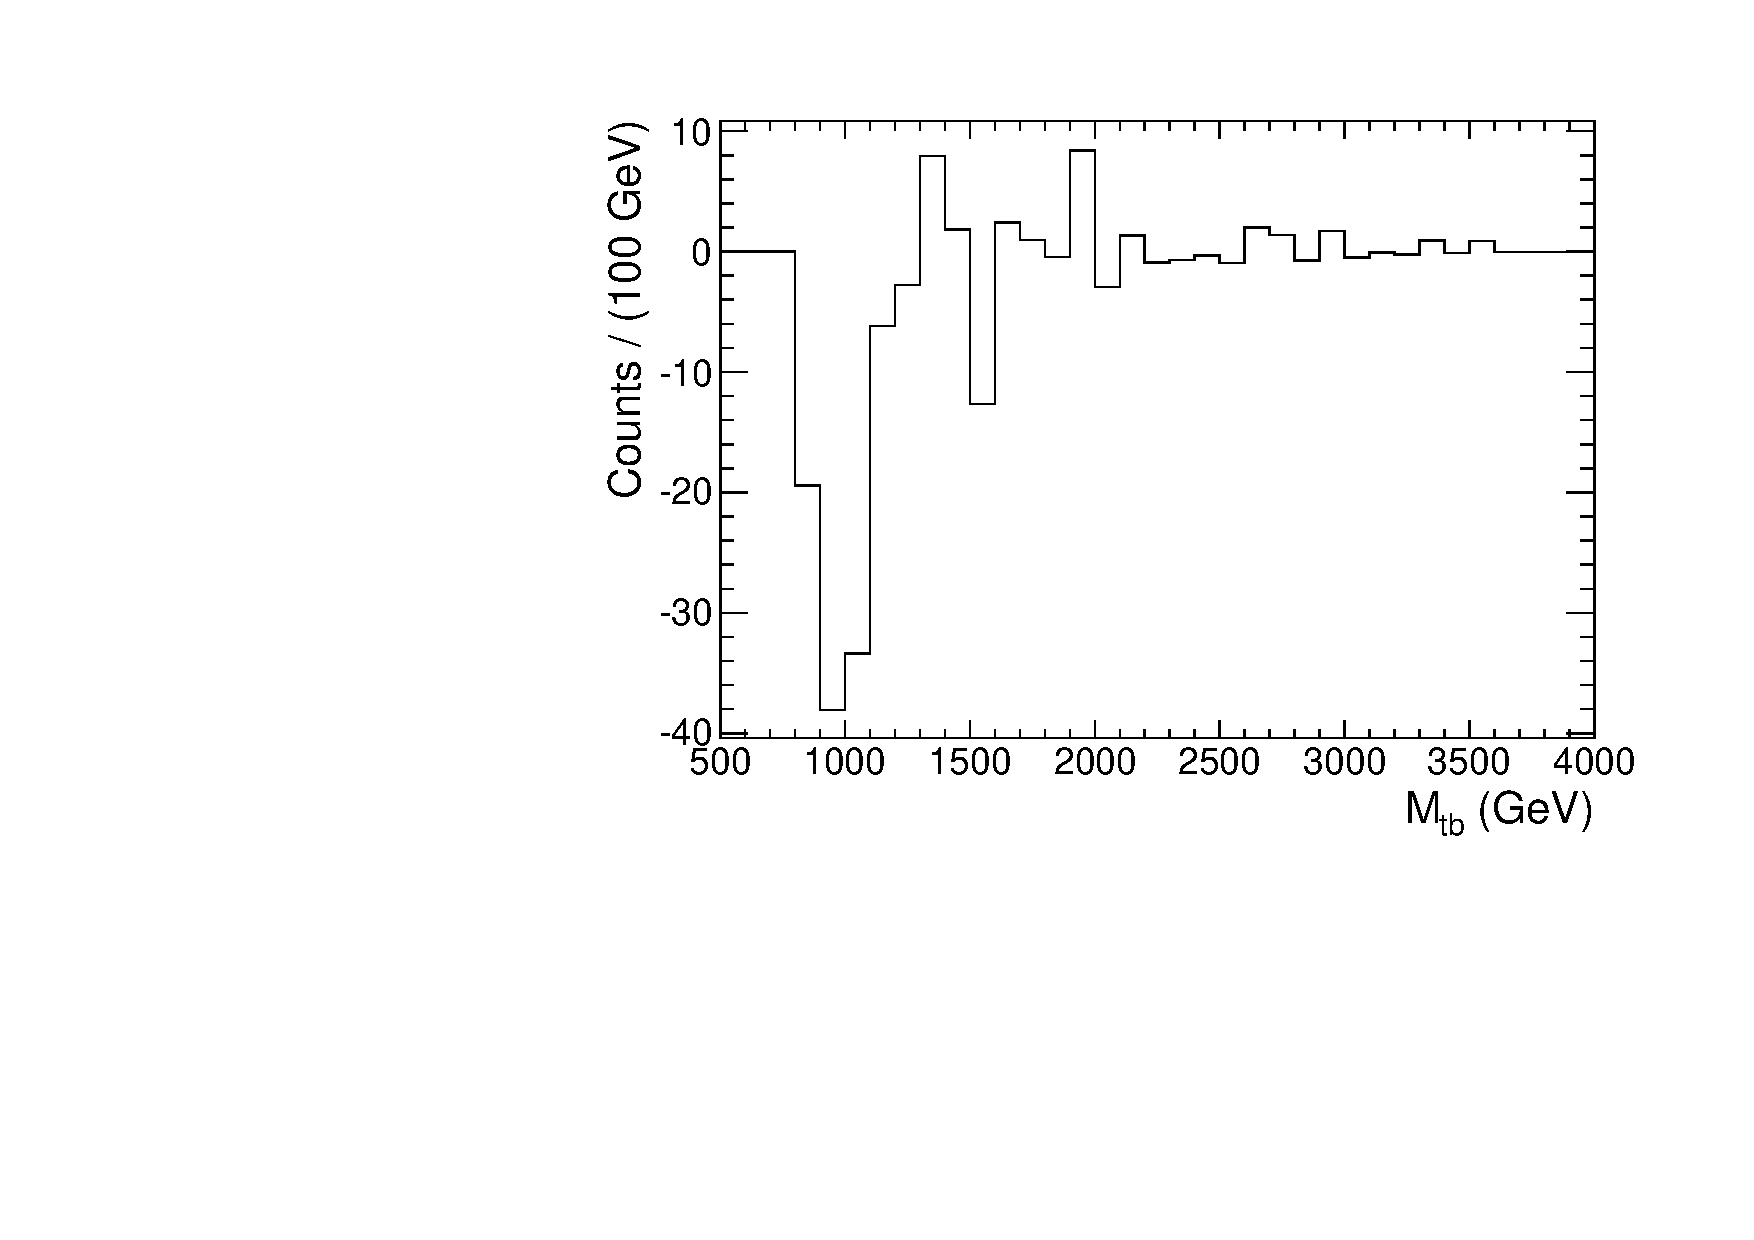
\includegraphics[width=1.0\textwidth]{figs/Mtb1dminusFS.pdf}}
\caption{
(a) Difference of the background estimation from three dimensional and two dimensional tagging rates
(b) Difference of the background estimation from second sideband selection and two dimensional tagging rates
}
\label{figs:sb2comp}
\end{center}
\end{figure}


\subsection{Signal Contamination Studies}
\label{sec:sigcont}
The following studies investigate signal contamination within our analysis.  These plots use the same color scheme seen in Figure \ref{figs:legend}.  
The signal contamination within the sideband used for extraction of the average b-tagging rate can be seen in Figure \ref{figs:trsigcont} (this is signal injected 
into the post b tagged plots in Figure \ref{figs:tagsandprobes8TeV}).  The signal contamination for the signal region can be seen in Figure \ref{figs:sigFS}.

There is also some signal contamination within the sideband cross checks described in Section \ref{sec:secondsideband}.  The signal contamination within Figure \ref{figs:NewMtbSB2} can be seen in Figure \ref{figs:sigSB2}, 
and the contamination in Figure \ref{figs:NewMtbSB3} can be seen in Figure \ref{figs:sigSB3}. 

\begin{figure}[Htcb]
\centering
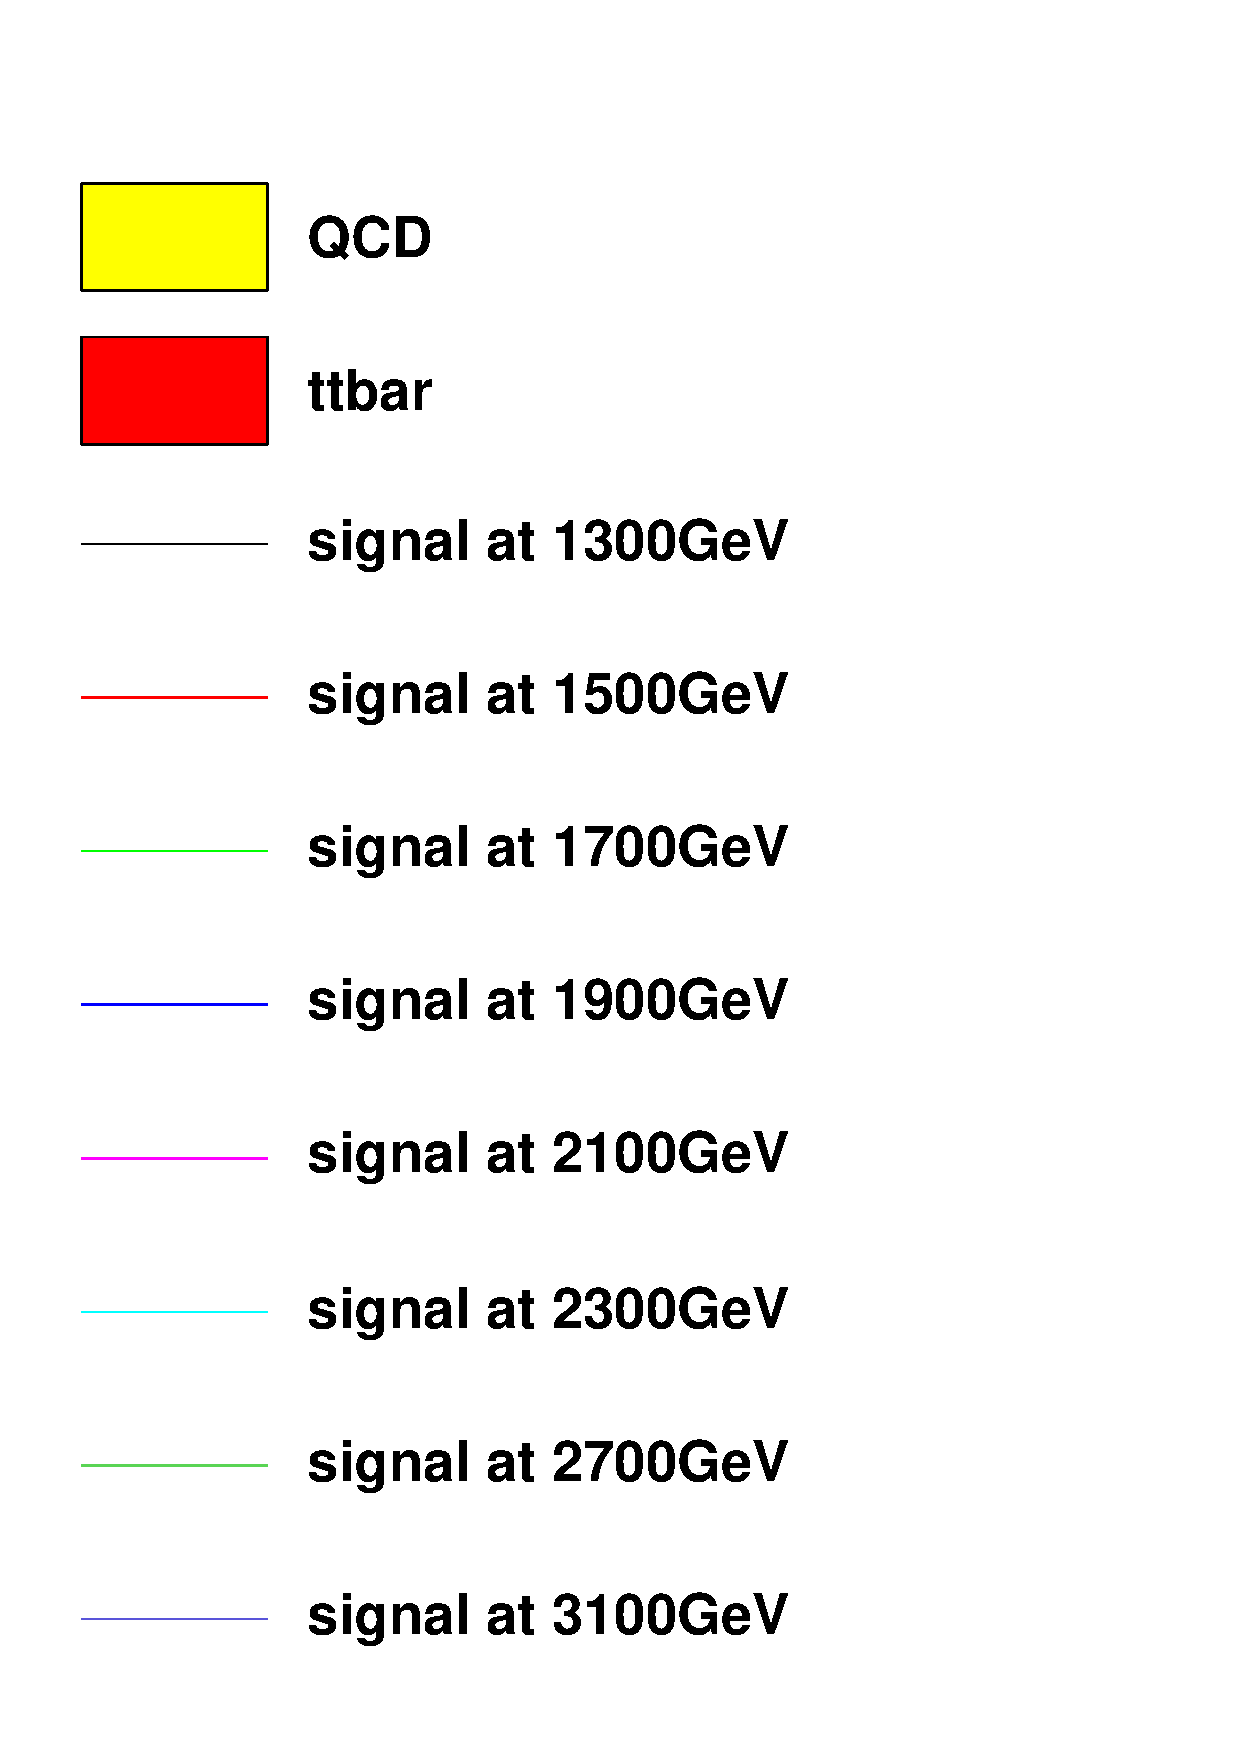
\includegraphics[width=0.45\textwidth]{figs/legend.pdf}
\caption{Legend for the following studies}
\label{figs:legend}
\end{figure}

\begin{figure}[Htcb]
\begin{center}
\subfigure{\label{figs:sceta1}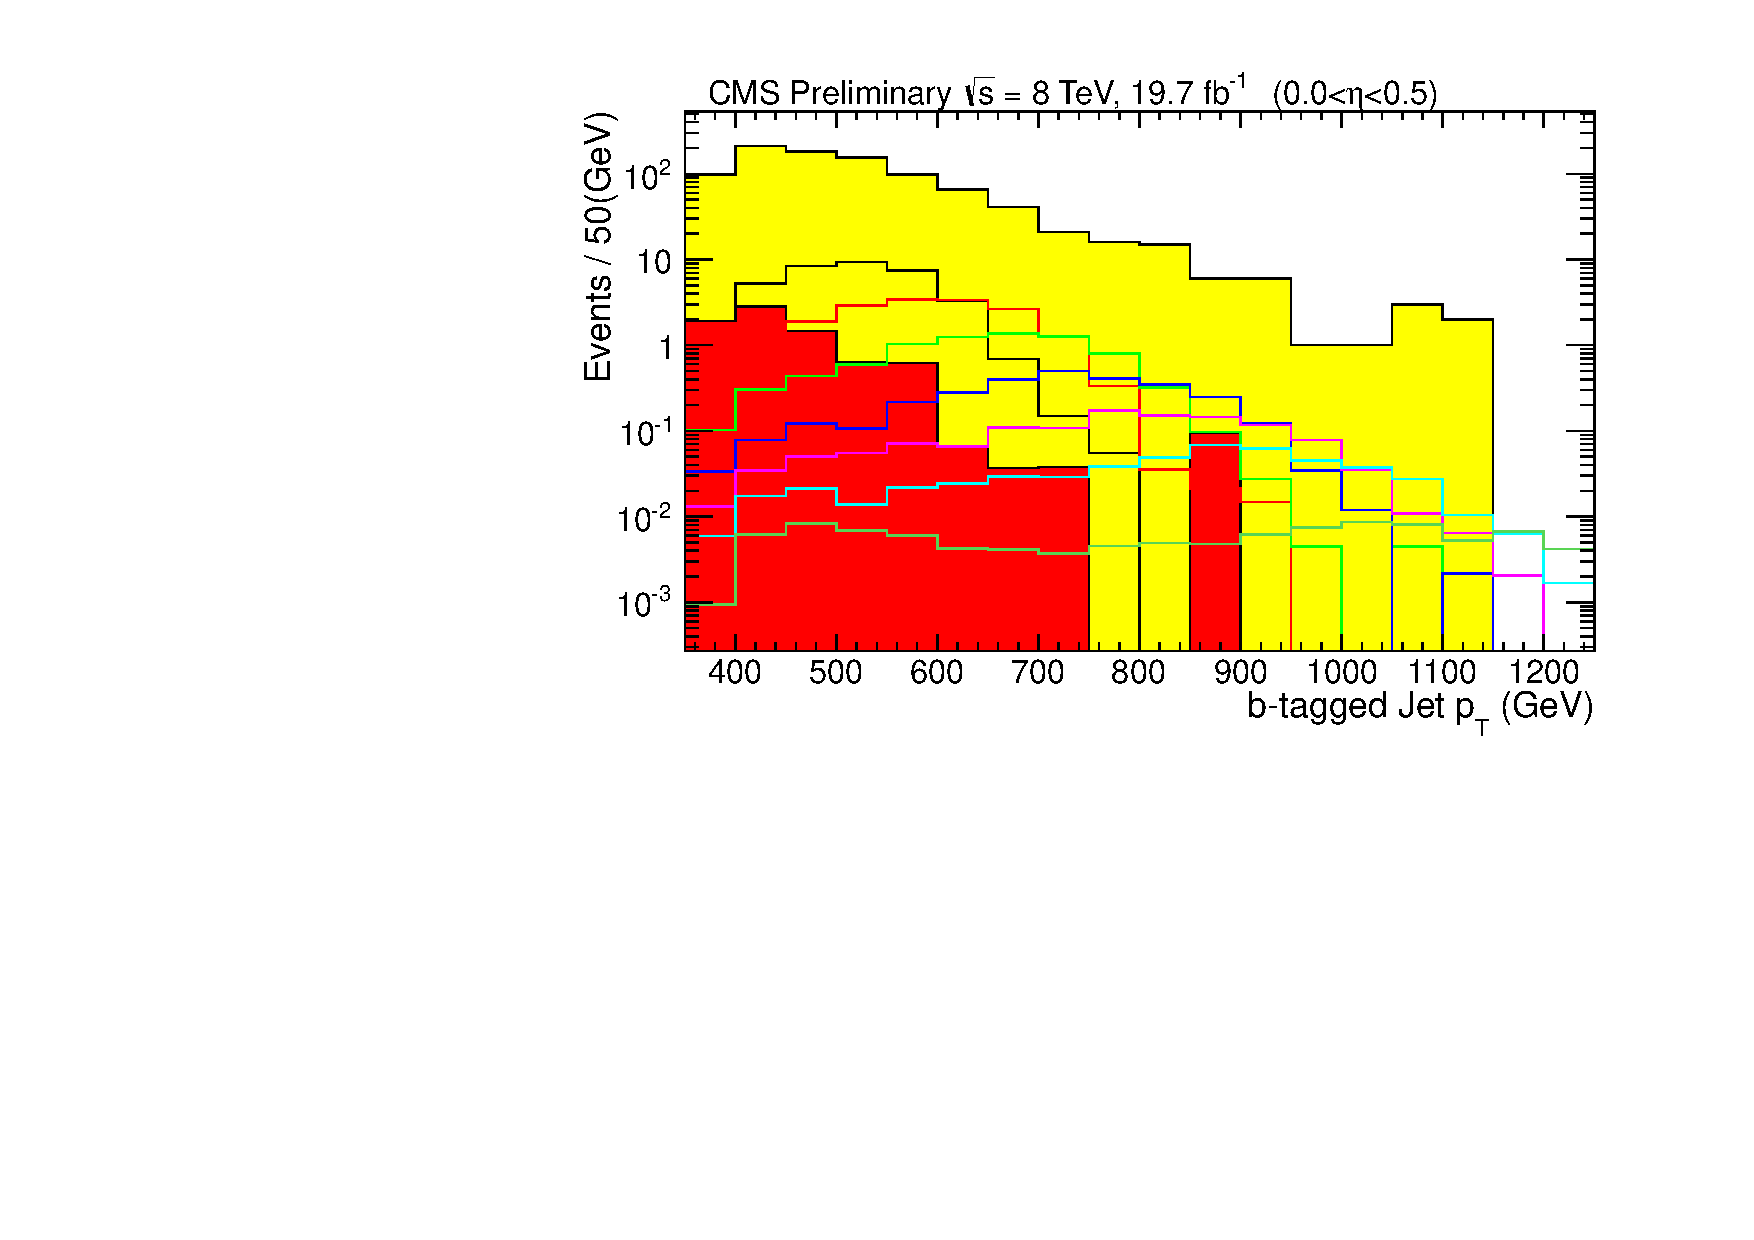
\includegraphics[width=0.7\textwidth]{figs/sigvsTReta1.pdf}}\\
\subfigure{\label{figs:sceta2}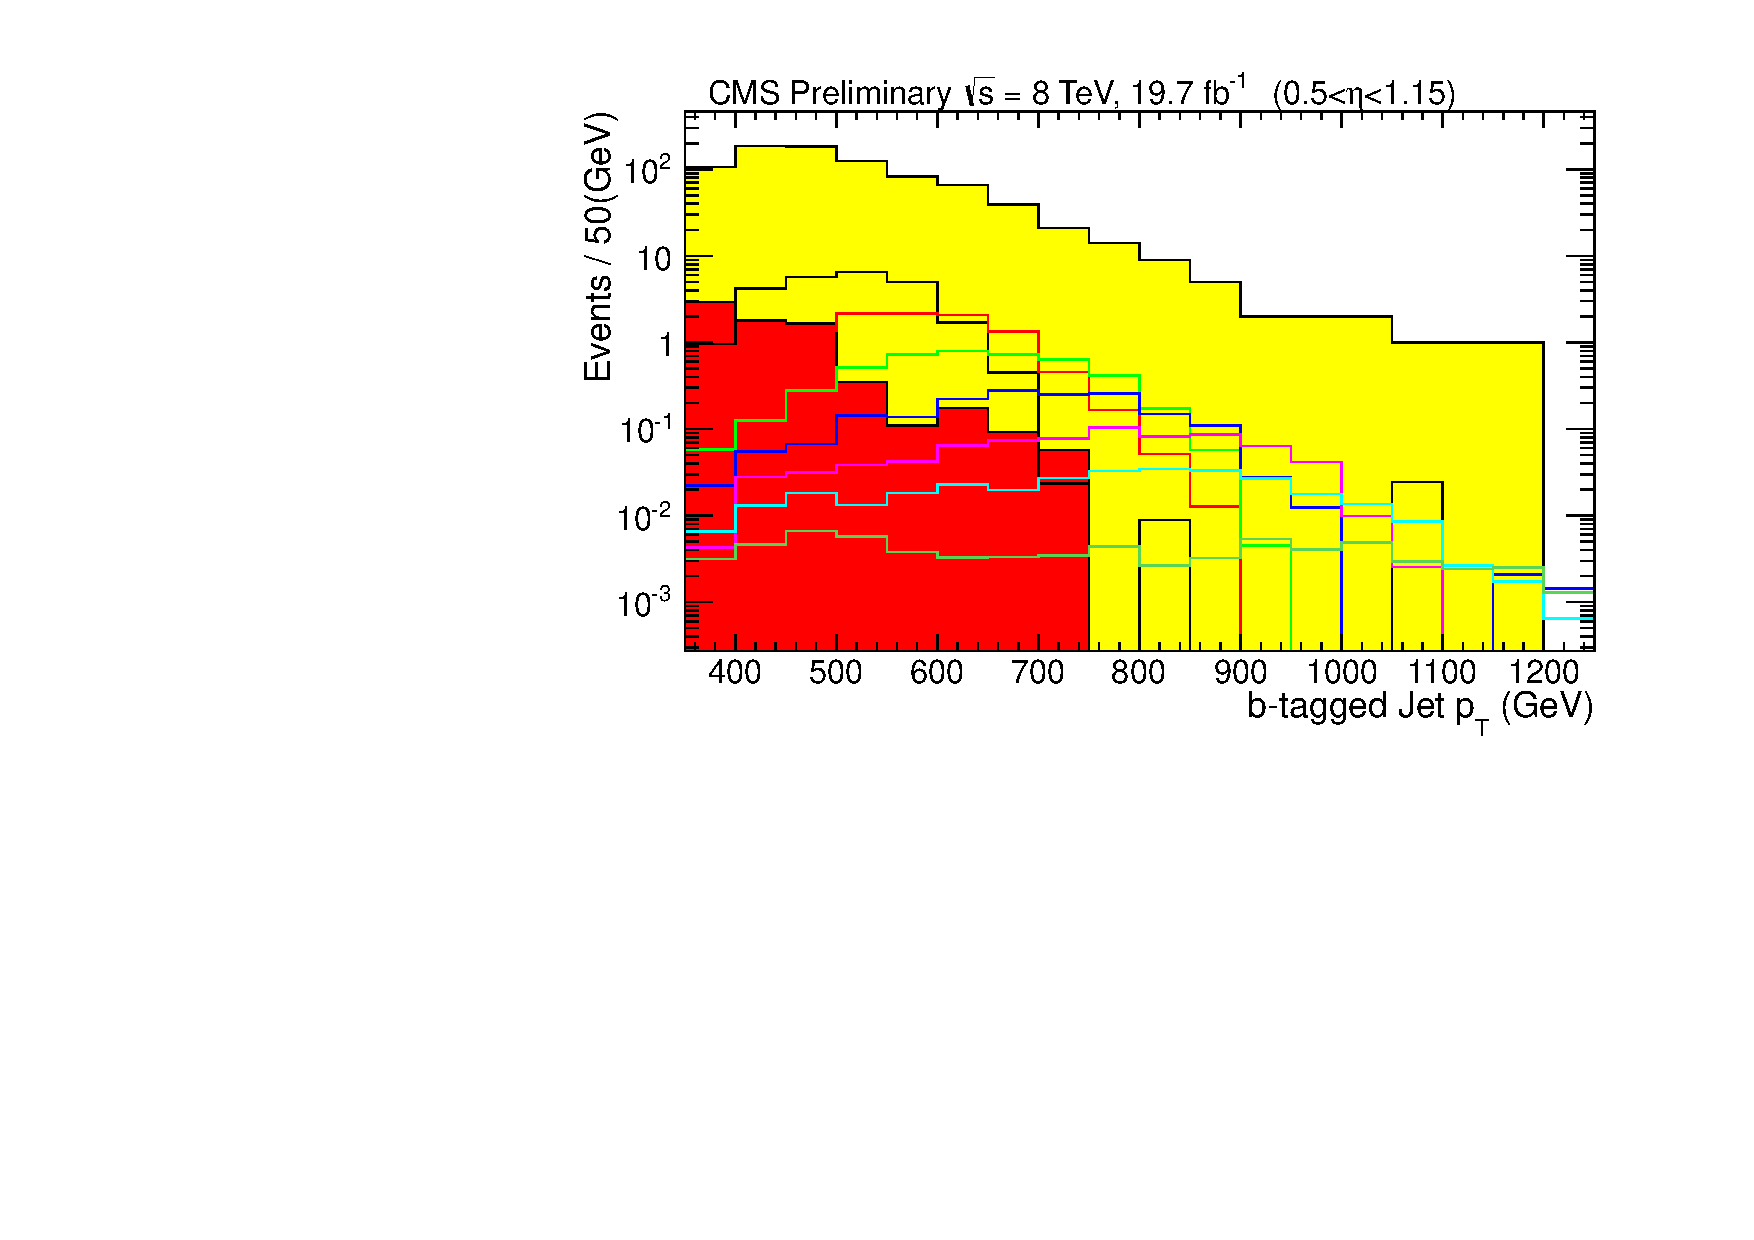
\includegraphics[width=0.7\textwidth]{figs/sigvsTReta2.pdf}}\\
\subfigure{\label{figs:sceta3}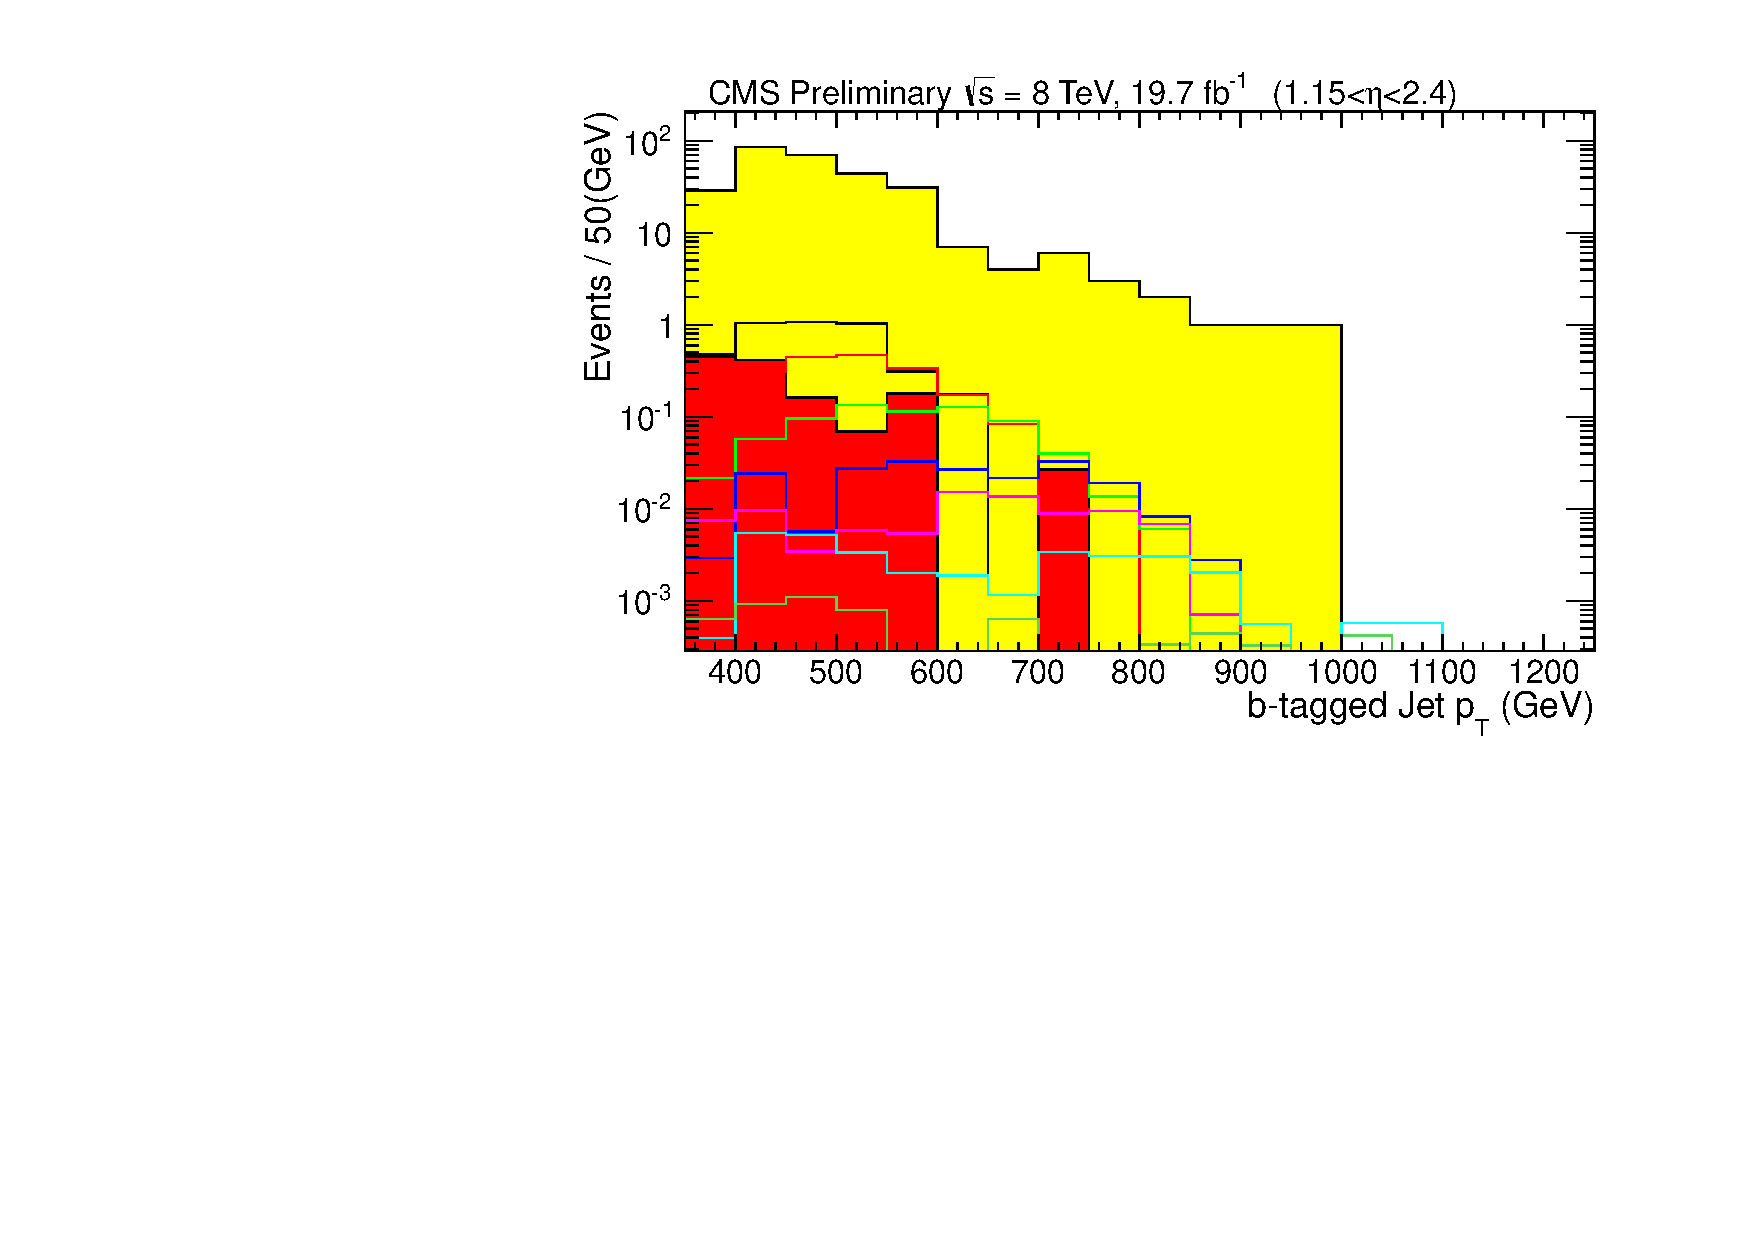
\includegraphics[width=0.7\textwidth]{figs/sigvsTReta3.pdf}}
\caption{
Signal contamination in the post b tagged sideband used to extract the average b-tagging rate
(a) Low $\eta$ region  
(b) Transition $\eta$ region 
(c) High $\eta$ region 
}
\label{figs:trsigcont}
\end{center}
\end{figure}

\begin{figure}[Htcb]
\centering
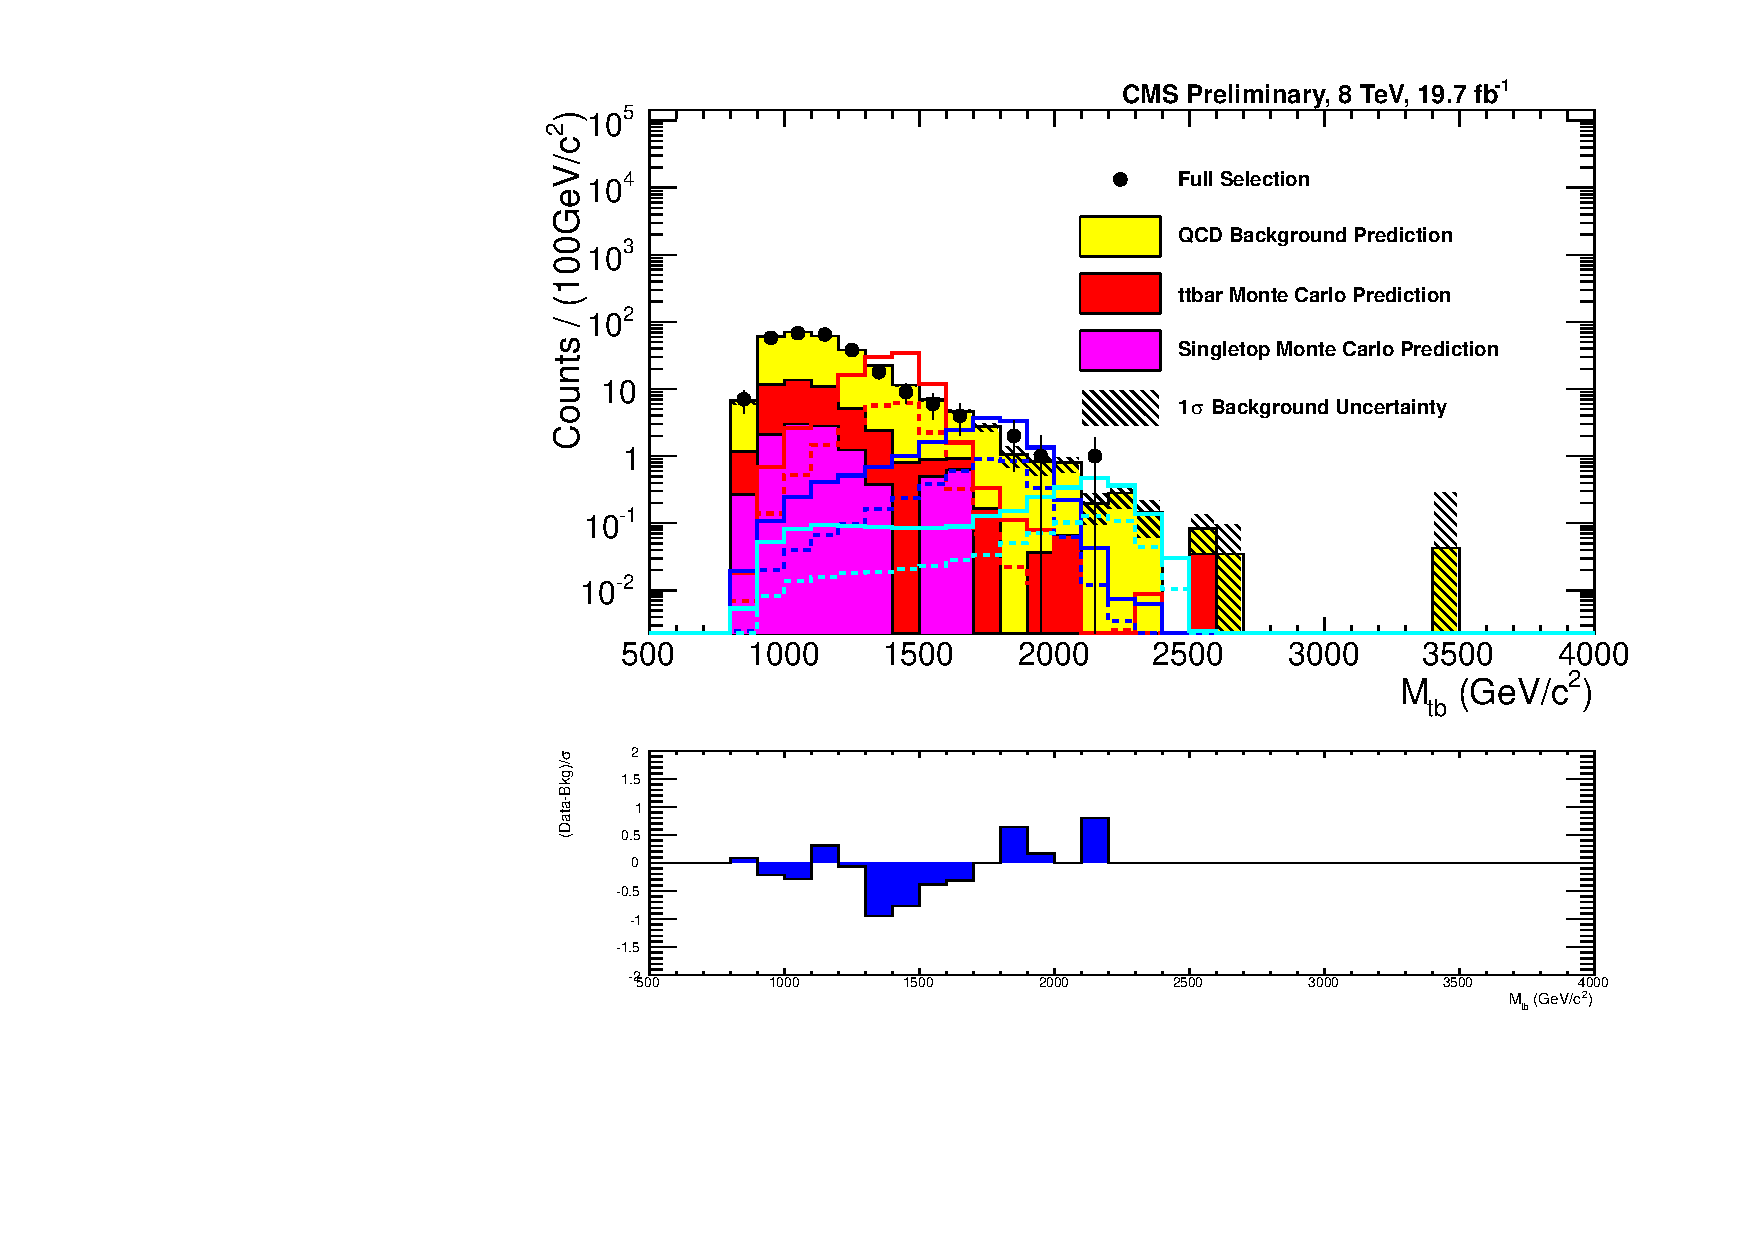
\includegraphics[width=1.0\textwidth]{figs/sigcontsemilog.pdf}
\caption{Signal contamination for the full selection.  The solid lines are the signal that passes the full selection.  The dashed lines are the signal that falls through the background estimate.}
\label{figs:sigFS}
\end{figure}

\begin{figure}[Htcb]
\centering
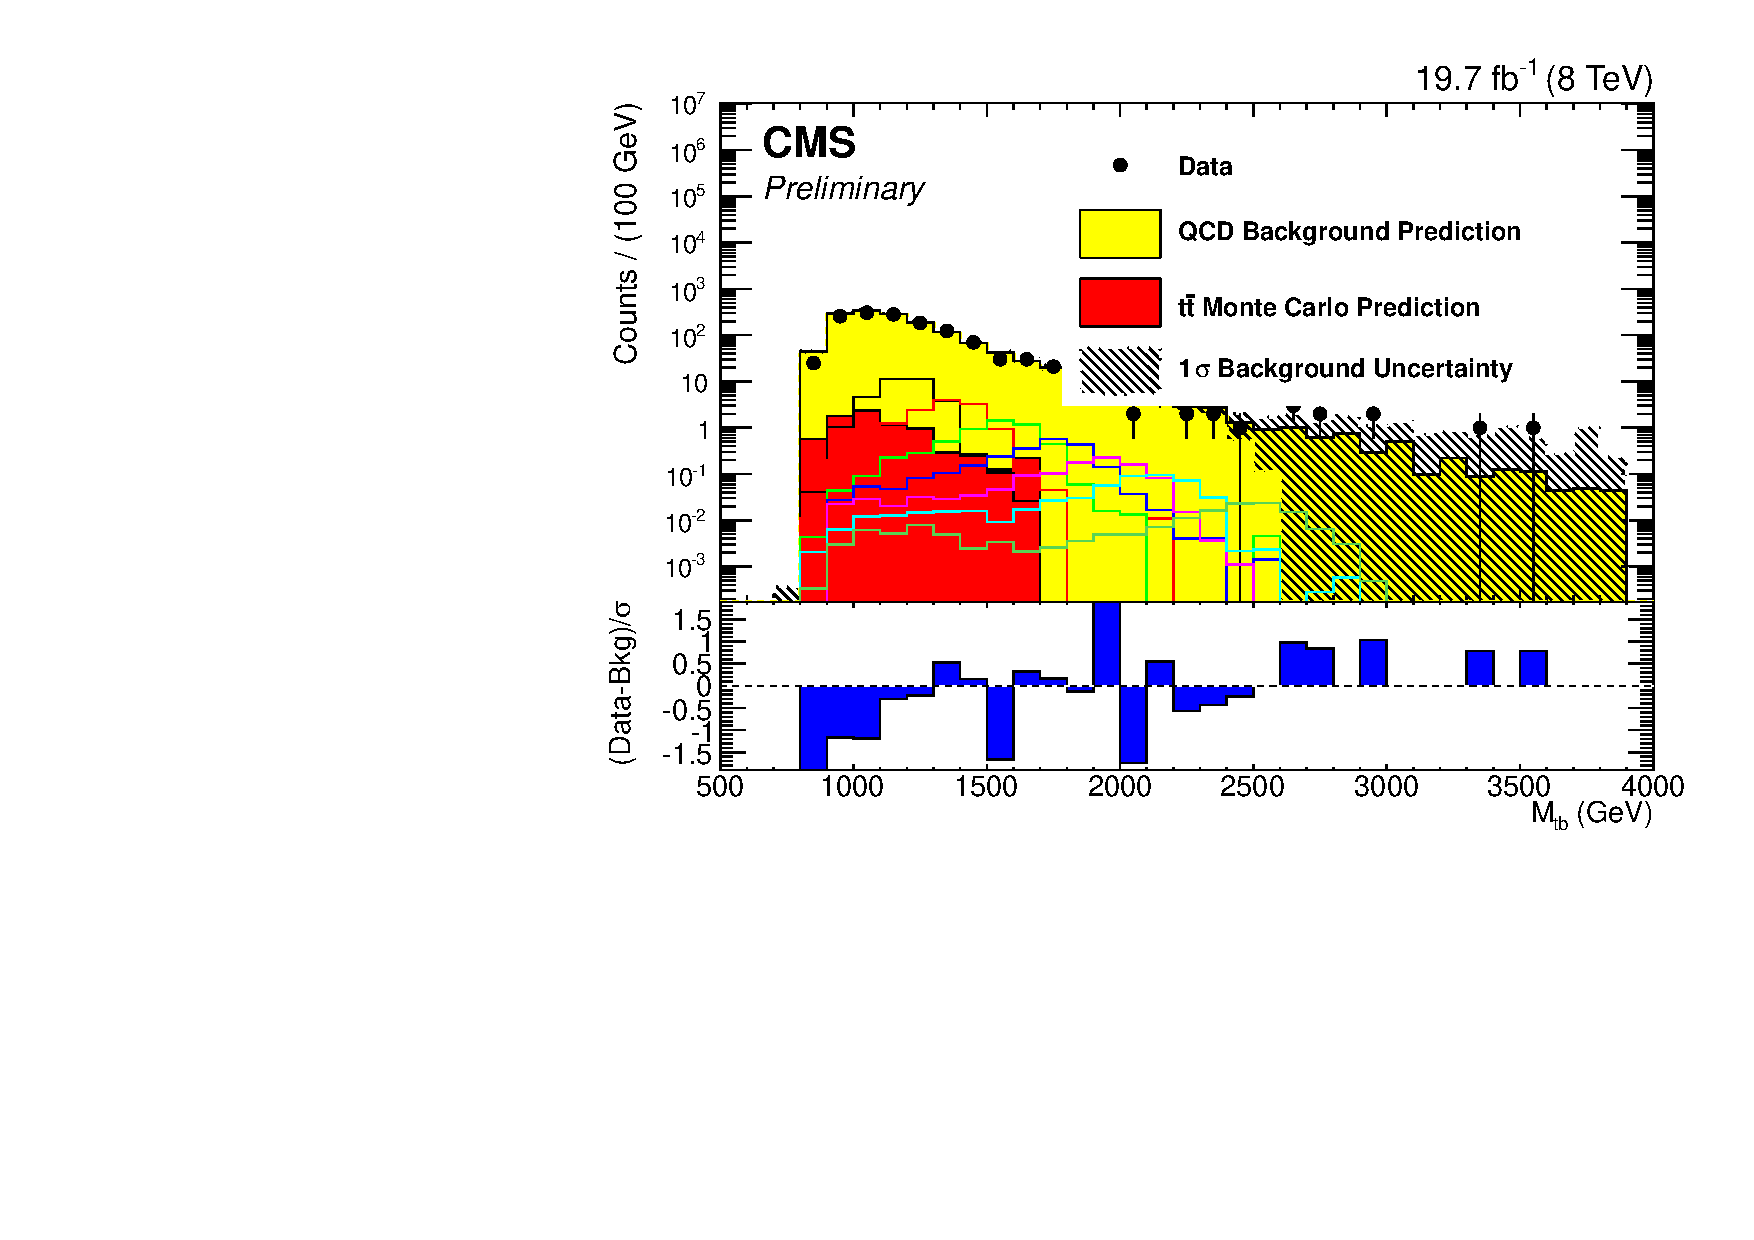
\includegraphics[width=1.0\textwidth]{figs/NewMtbSB2semilogwithsignal.pdf}
\caption{Signal contamination in sideband}
\label{figs:sigSB2}
\end{figure}

\begin{figure}[Htcb]
\centering
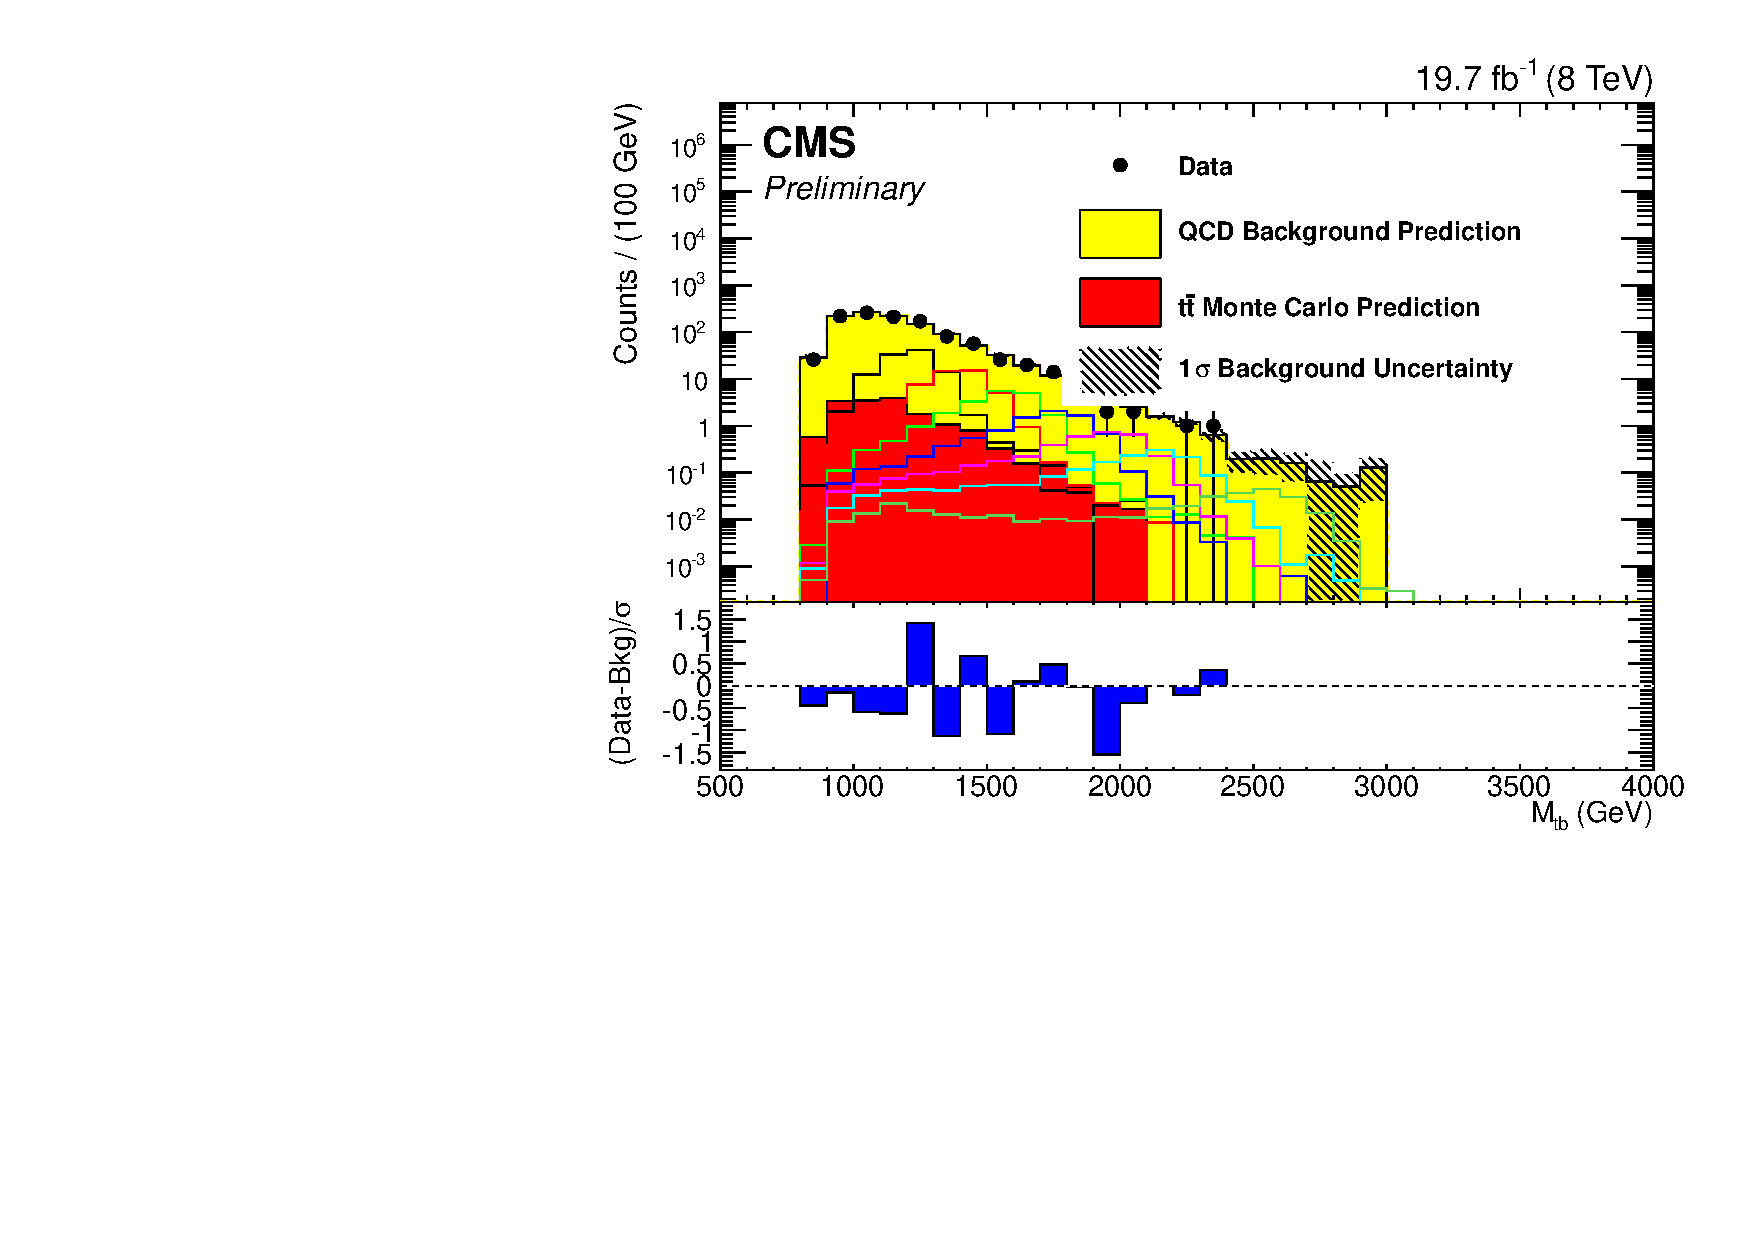
\includegraphics[width=1.0\textwidth]{figs/NewMtbSB3semilogwithsignal.pdf}
\caption{Signal contamination in sideband}
\label{figs:sigSB3}
\end{figure}


\subsection{Generalized Coupling Signal Sample Comparison}
\label{sec:sigcont}

\begin{figure}[htcb]
\begin{center}
\subfigure{\label{figs:gen1}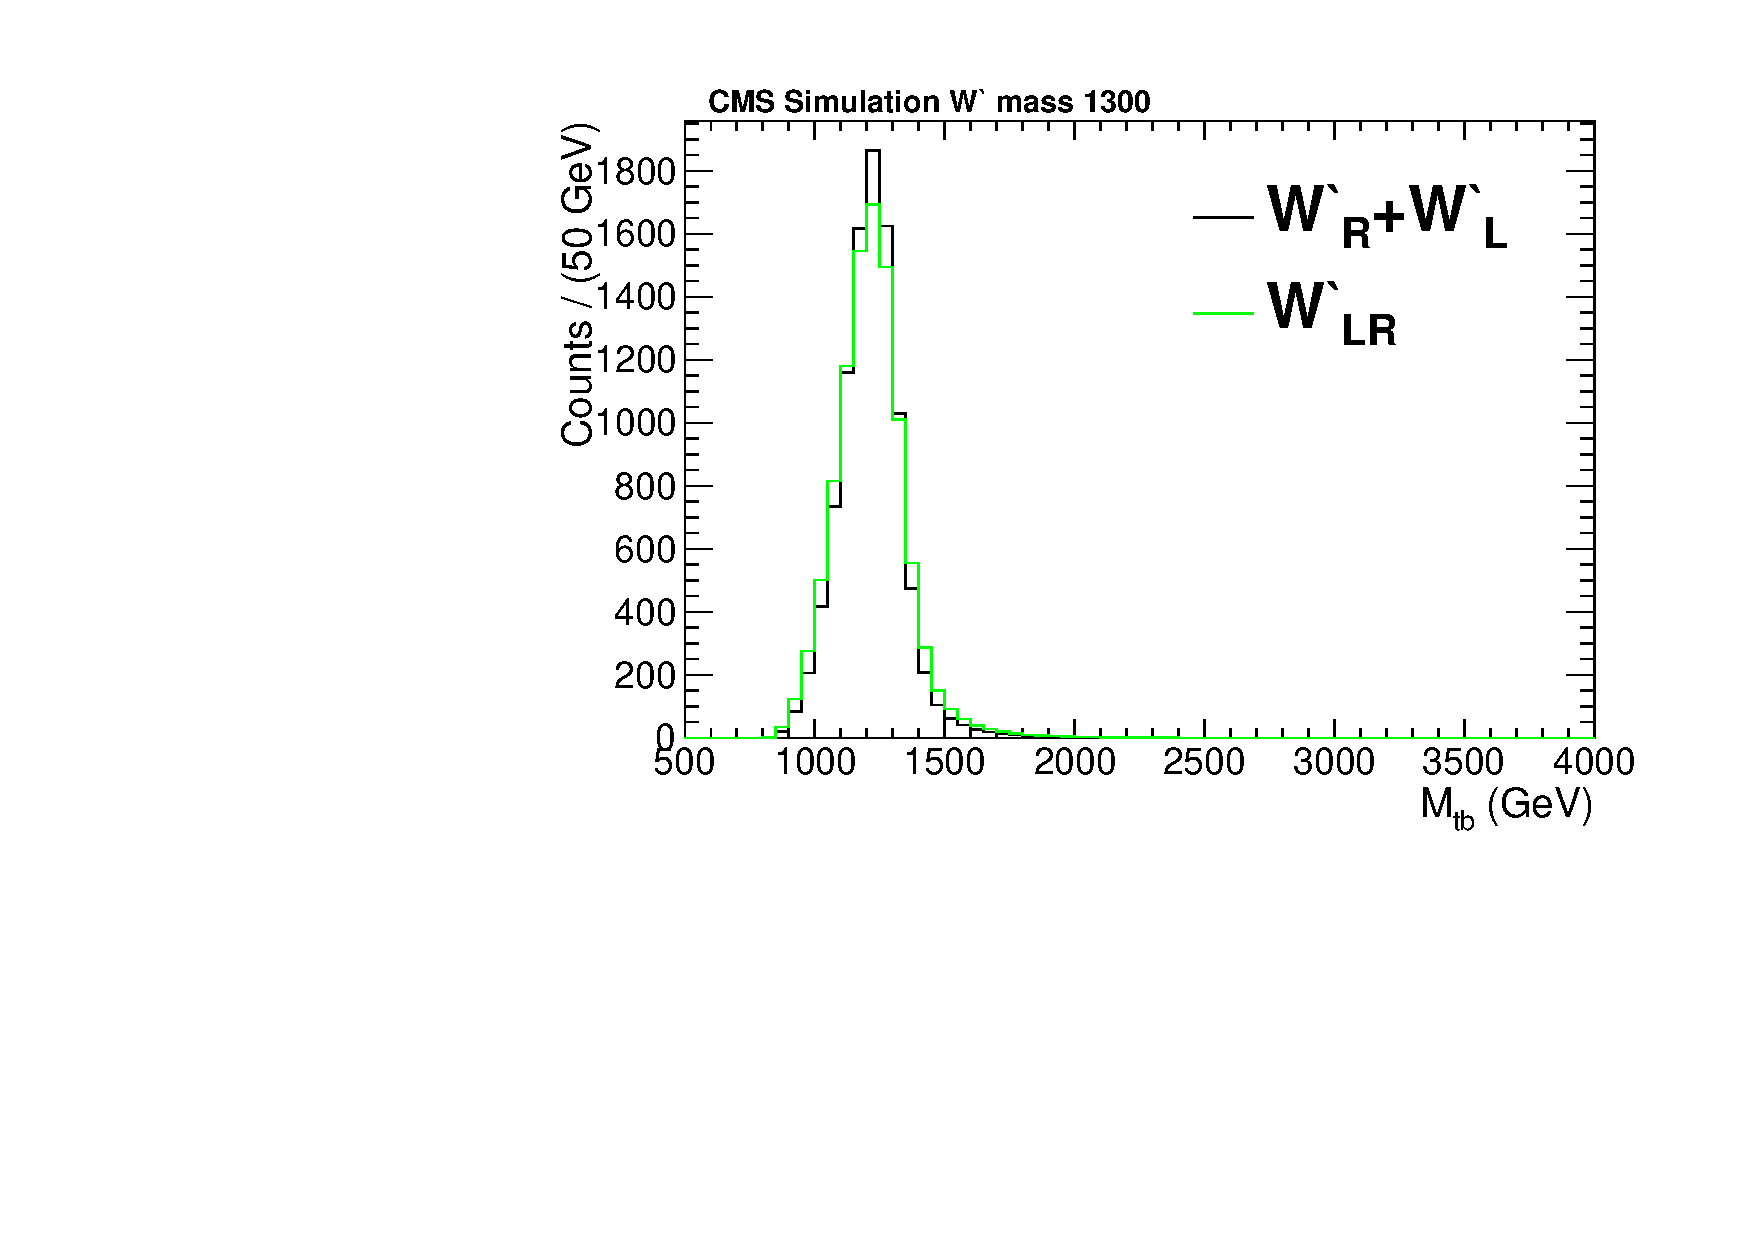
\includegraphics[width=0.7\textwidth]{figs/SignalmixedvsLplusR1300.pdf}}\\
\subfigure{\label{figs:gen2}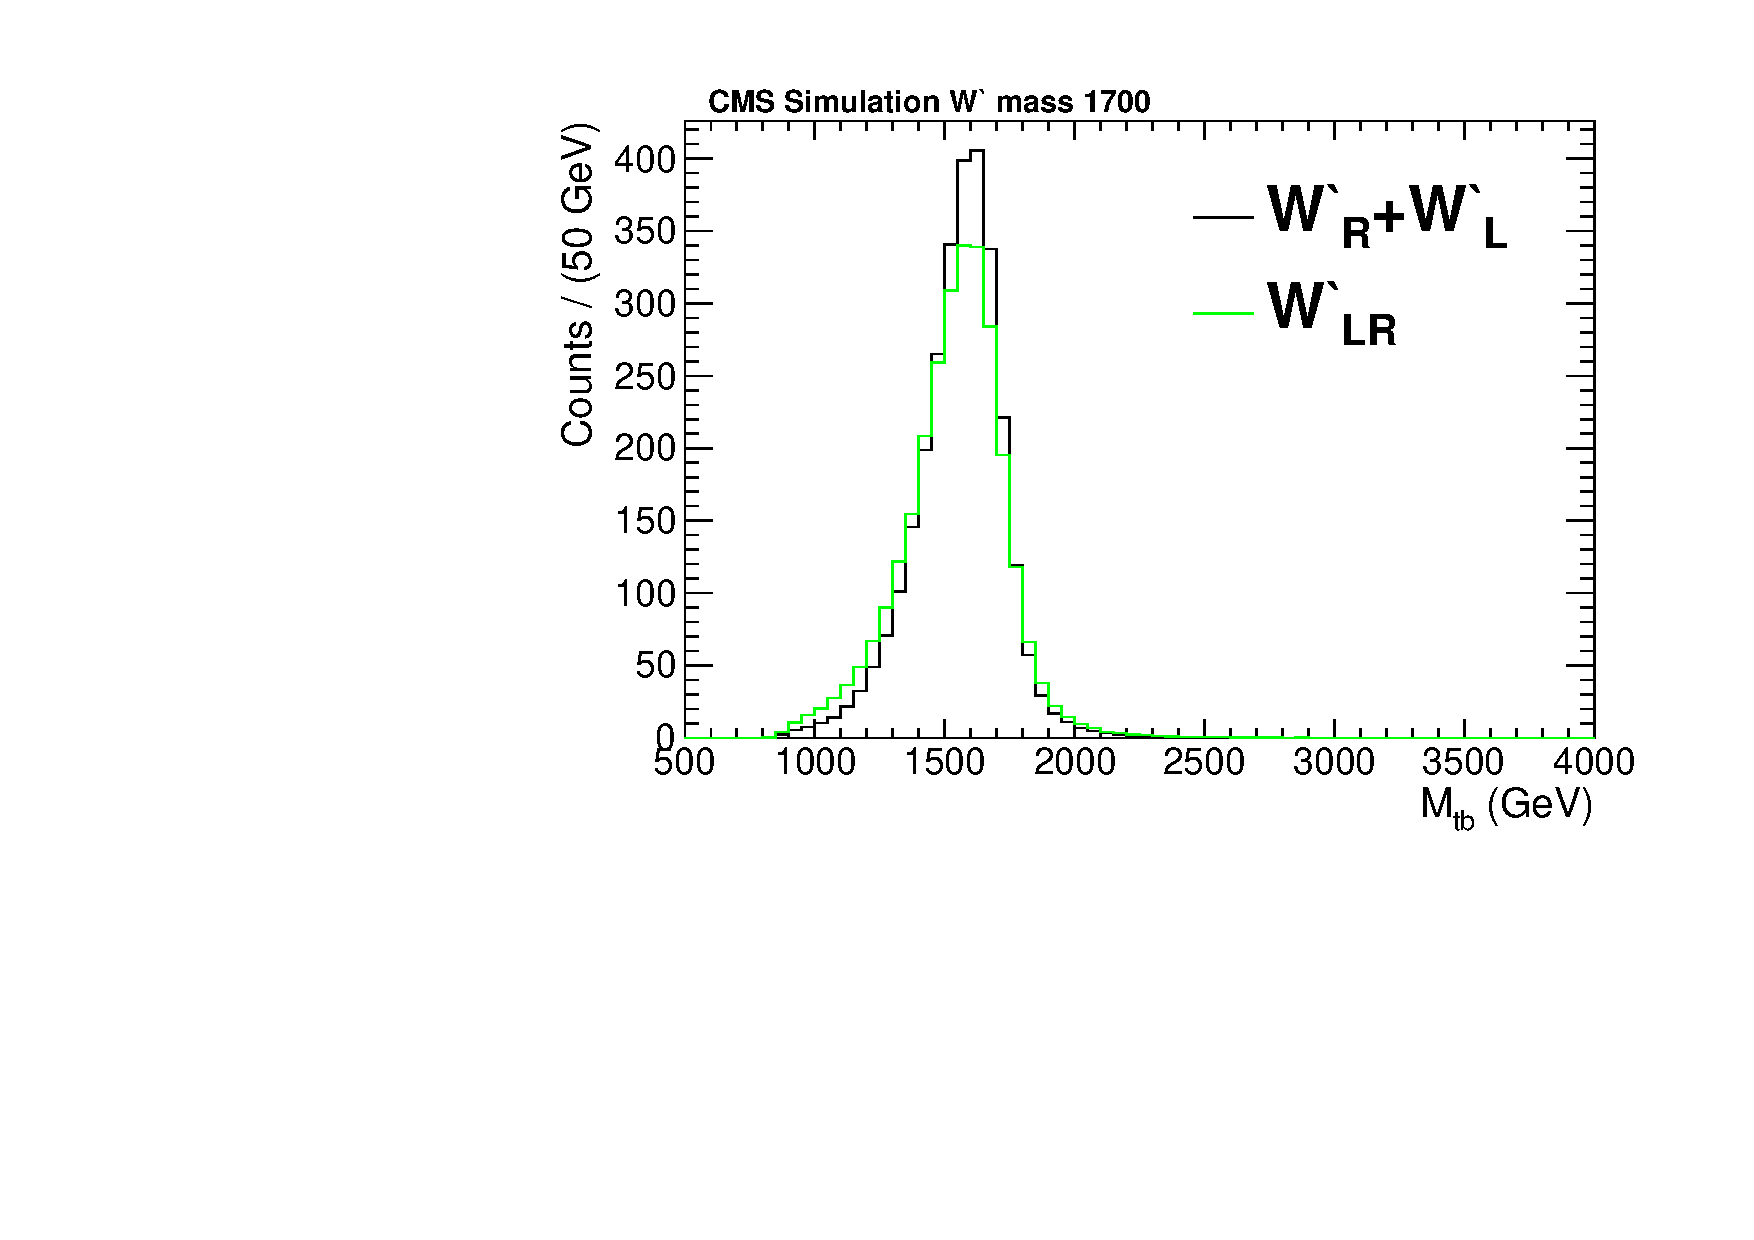
\includegraphics[width=0.7\textwidth]{figs/SignalmixedvsLplusR1700.pdf}}\\
\subfigure{\label{figs:gen3}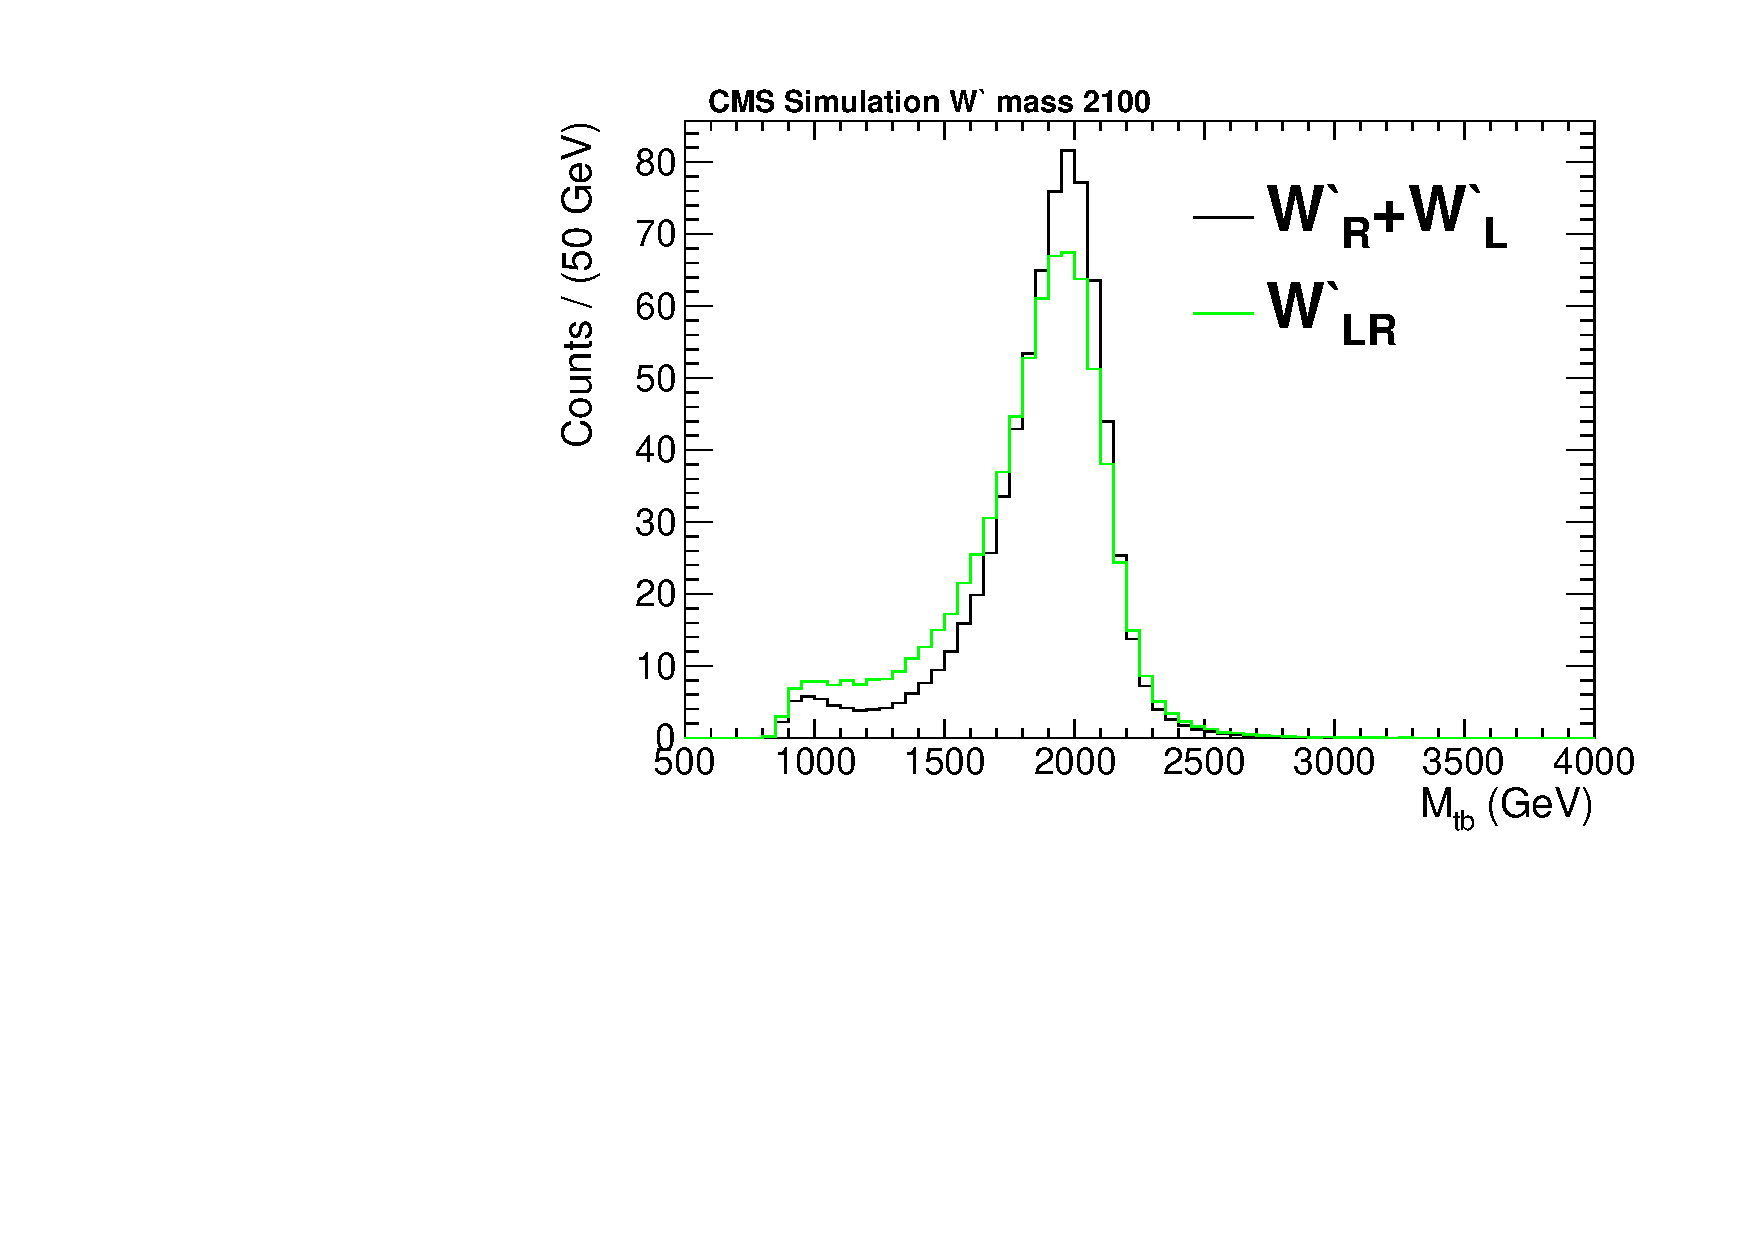
\includegraphics[width=0.7\textwidth]{figs/SignalmixedvsLplusR2100.pdf}}
\caption{
$M_{tb}$ spectrum of events comparing the summed $\wpr_{R}$ and $\wpr_{L}$ templates to the $\wpr_{LR}$ template.  The selection used for these plots only includes the kinematic cuts.
}
\label{figs:Gencomp1}
\end{center}
\end{figure}

%\section{Top Tagging Scale Factor Studies in Signal MC}
%\label{sec:ttsfsigandttbar}
%We study the applicability of the top tagging scale factor as derived from $\ttbar$ MC.  Figures \ref{figs:effr1} and \ref{figs:effr2} shows top tagging efficiency comparisons as parameterized in $\pt$ and $\eta$.

%\begin{figure}[Htcb]
%\centering
%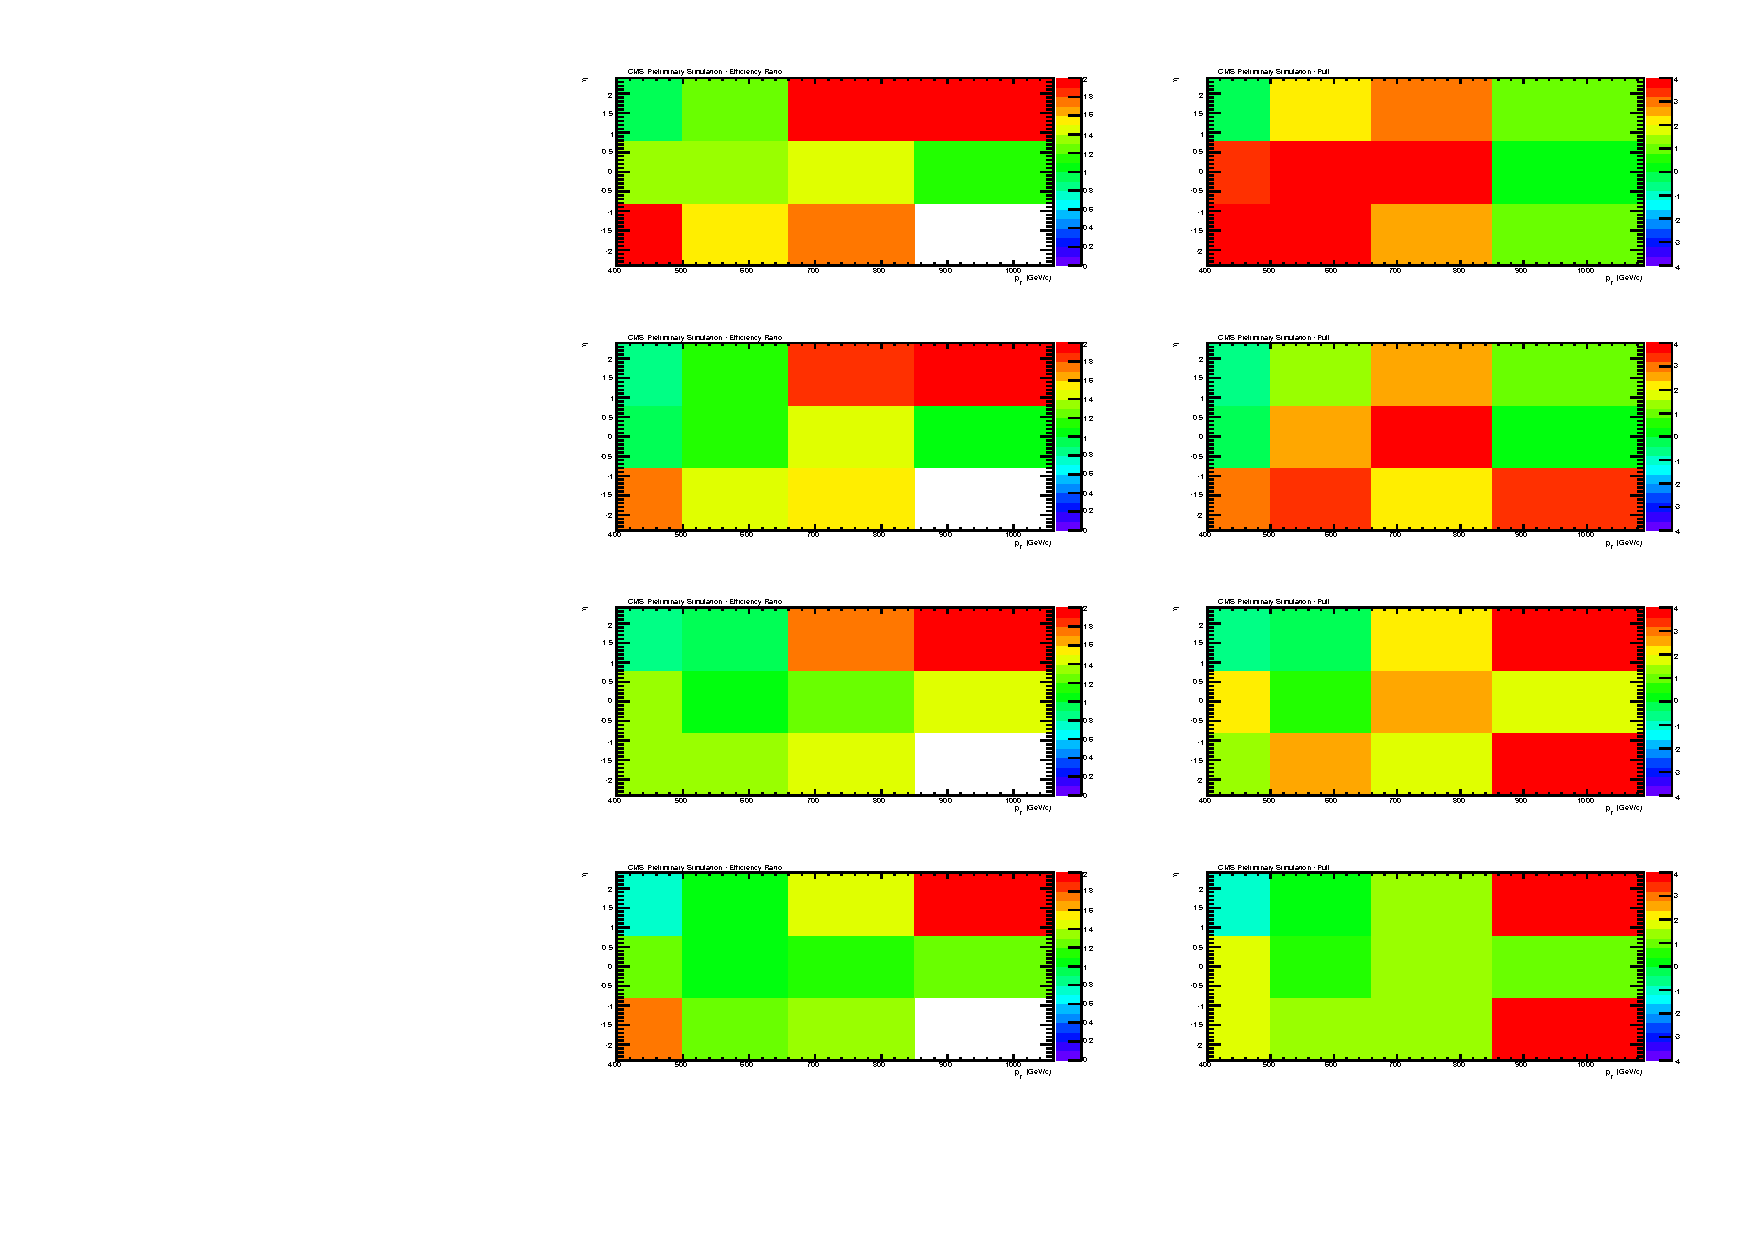
\includegraphics[width=1.0\textwidth]{figs/effratioandpull1.pdf}
%\caption{Study of the applicability of the top tagging scale factor to signal MC.  Plots on the left are the ratio of top tagging efficiency in signal to $\ttbar$.  Plots on the right are the pull distributions (($Eff_{signal} - EFF_{ttbar}$)/$\sigma$). 
%Where $\sigma$ is the statistical uncertainty.  From top to bottom we study $\wpr$ MC mass points from 1300 to 3100 $~\GeV$}
%\label{figs:effr1} - 
%\end{figure}

%\begin{figure}[Htcb]
%\centering
%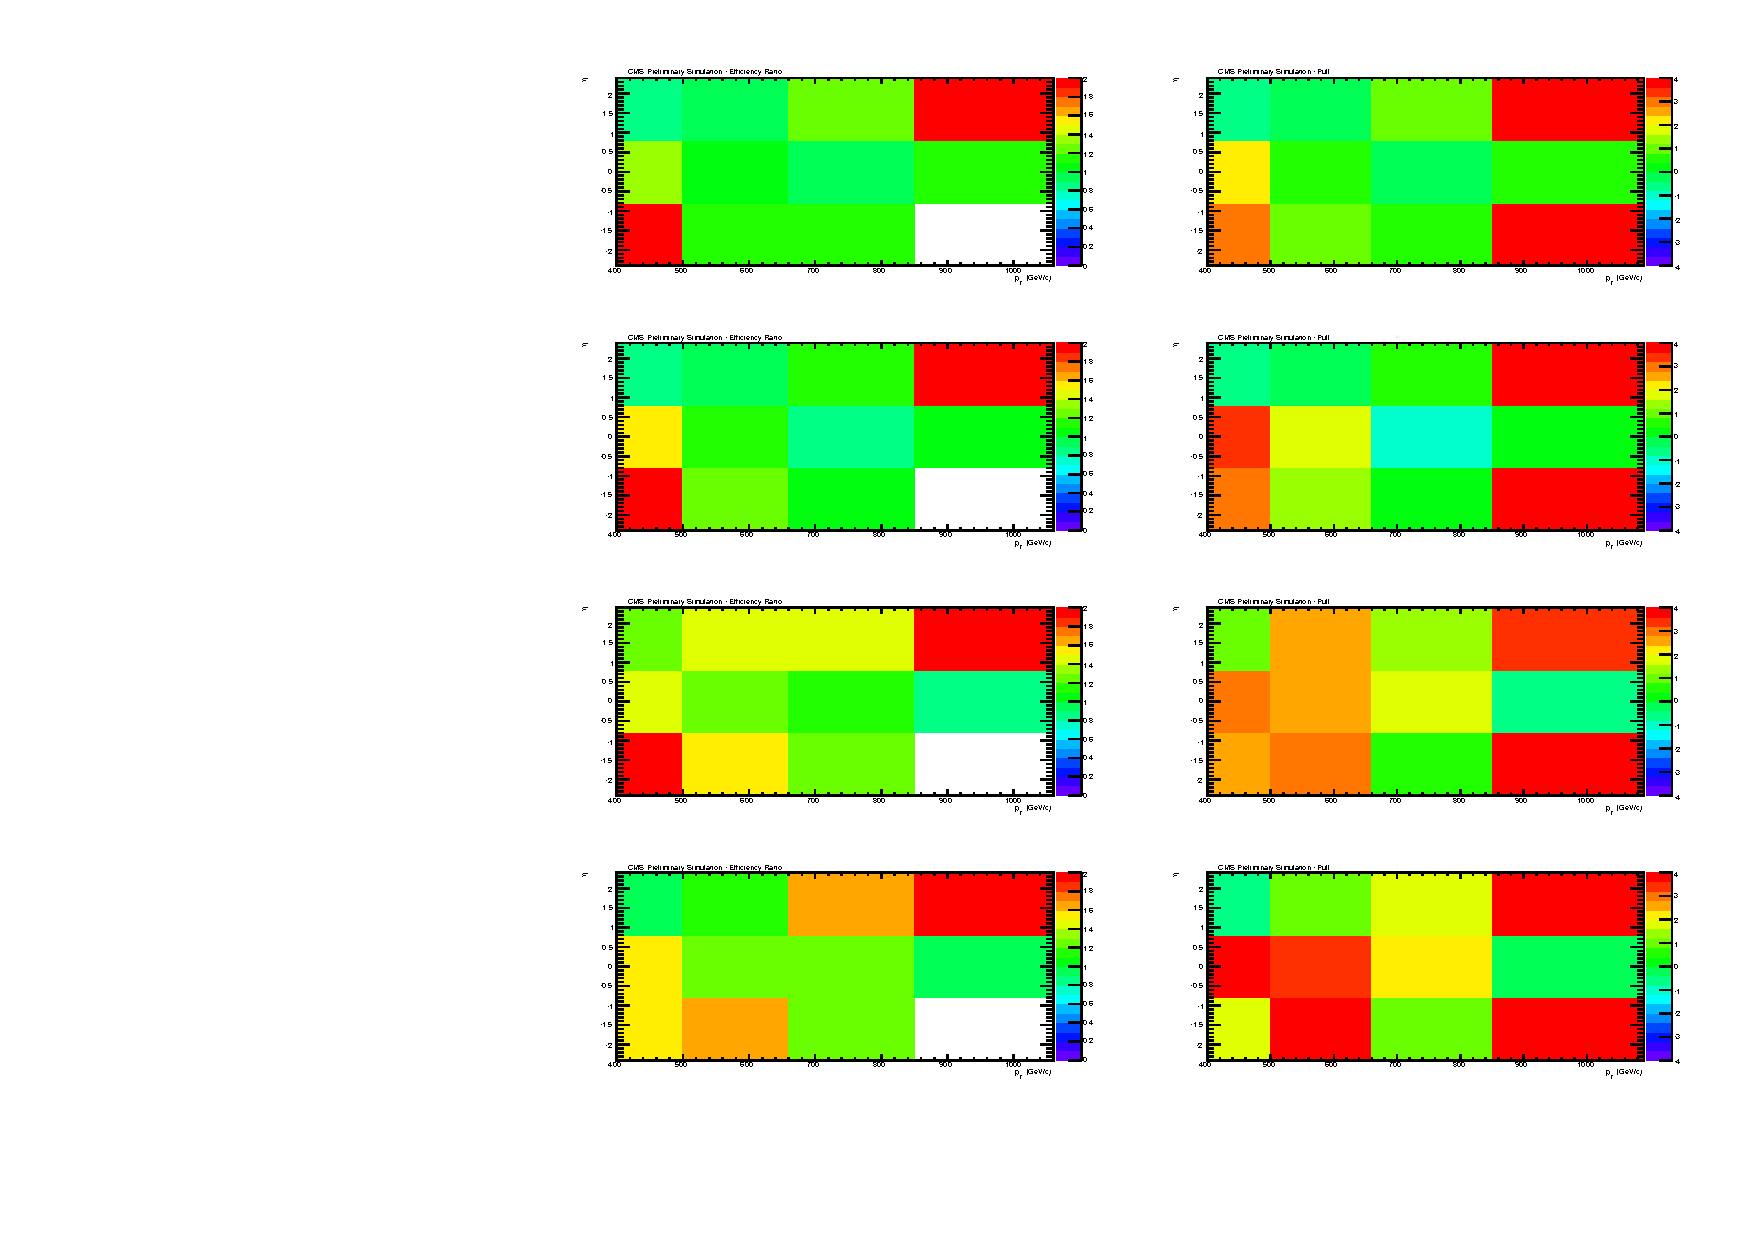
\includegraphics[width=1.0\textwidth]{figs/effratioandpull2.pdf}
%\caption{Study of the applicability of the top tagging scale factor to signal MC.  Plots on the left are the ratio of top tagging efficiency in signal to $\ttbar$.  Plots on the right are the pull distributions (($Eff_{signal} - EFF_{ttbar}$)/$\sigma$). 
%Where $\sigma$ is the statistical uncertainty.  From top to bottom we study $\wpr$ MC mass points from 1300 to 3100 $~\GeV$}
%\label{figs:effr2} - 
%\end{figure}



\section{$\bs$ Search}
\label{sec:appendix}
Figure \ref{figs:bsqcdtr} shows a comparison of the top-mistagging rate extracted from the W-tagging sideband described in Section \ref{sec:qcdBackgroundEstimationProcedure} and the top-mistagging rate extracted from the signal region.  
This plot is taken from QCD MC.

\begin{figure}[htcb]
\centering
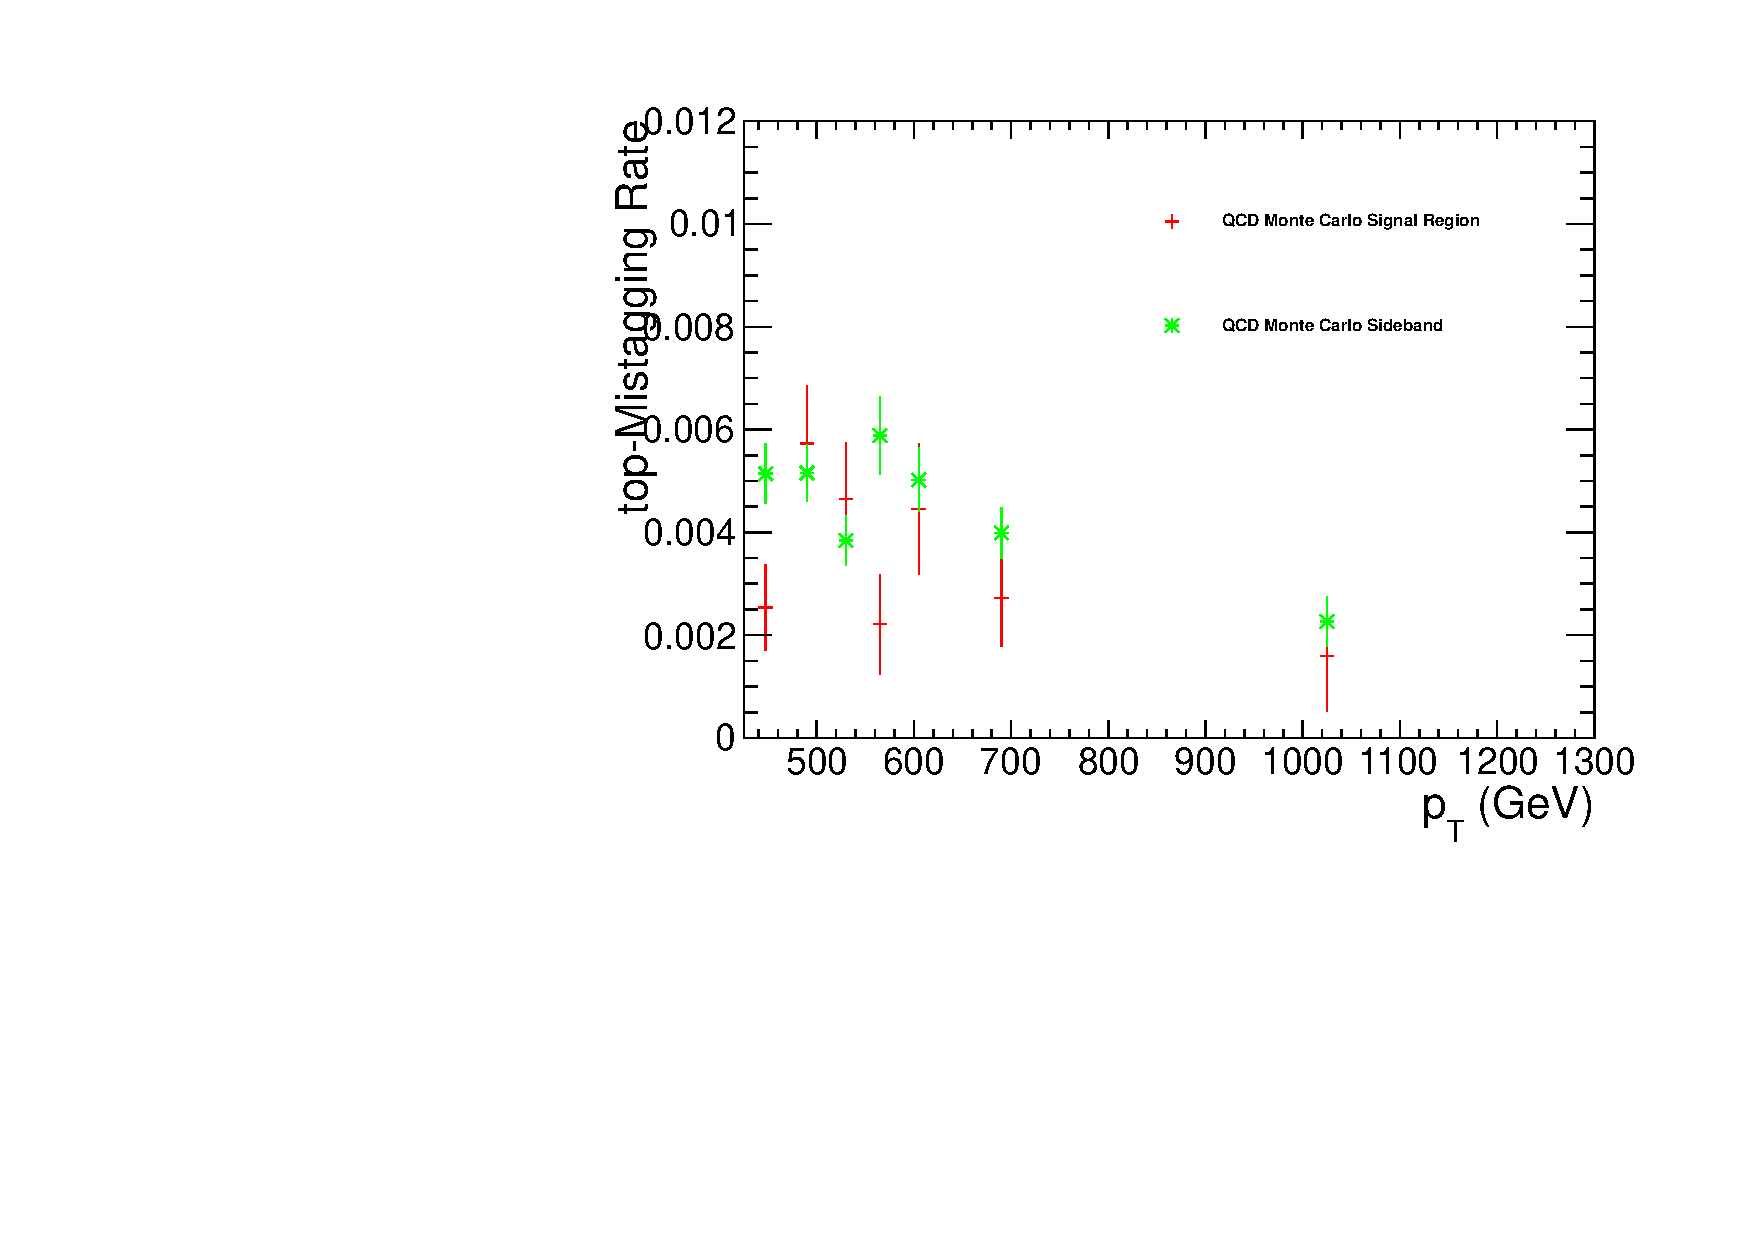
\includegraphics[width=1.0\textwidth]{AN-14-049/figs/qcdtrcomp.pdf}
\caption{ 
A QCD MC comparison of the top-mistagging rate extracted from the W-tagging sideband and the top-mistagging rate extracted from the signal region.  The QCD MC quickly runs out of statistics when 
full top-tagging is applied.}
\label{figs:bsqcdtr}
\end{figure} 



\begin{sidewaystable}[htcb]
\begin{center}
\begin{small}
\bf{Rate Effects of Systematic Uncertainties}\\
\scalebox{0.4}{

\begin{tabular}{|c||ccccccccccccc|}
\hline\hline 
Sample & B-tagging & Mass & Mistag & PDF & Pileup & QCD Rate el & QCD Rate mu & MET & Lepton ID & Isolation & Trigger & W+Jets Rate el & W+Jets Rate mu  \\ 
\hline 
WJets & +4.09,-4.14 & --- & +14.42,+9.44 & +41.28,+27.02 & -0.36,+0.30 & --- & --- & -0.00,-0.00 & +0.26,-0.26 & +0.00,+0.00 & +0.40,-0.36 & +45.00,-31.03 & --- \\ 
\hline 
ZJets & +3.37,-3.41 & --- & +8.95,+5.88 & +8.53,-7.33 & +0.99,+0.20 & --- & --- & +0.00,-0.00 & +0.32,-0.29 & +0.00,+0.00 & +0.54,-0.46 & --- & --- \\ 
\hline 
$M_{\bs=1000}$ & +2.89,-2.99 & --- & +0.17,+0.11 & +21.15,-17.64 & -0.15,+0.14 & --- & --- & +0.00,-0.00 & +0.17,-0.17 & +0.00,+0.00 & +0.26,-0.25 & --- & --- \\ 
\hline 
$M_{\bs=1100}$ & +2.87,-2.99 & --- & +0.21,+0.14 & +24.18,-19.44 & +0.10,-0.12 & --- & --- & -0.00,-0.00 & +0.18,-0.18 & +0.00,+0.00 & +0.27,-0.26 & --- & --- \\ 
\hline 
$M_{\bs=1200}$ & +2.83,-2.96 & --- & +0.22,+0.15 & +26.63,-21.11 & +0.17,-0.19 & --- & --- & -0.00,-0.00 & +0.17,-0.17 & +0.00,+0.00 & +0.26,-0.25 & --- & --- \\ 
\hline 
$M_{\bs=1300}$ & +2.83,-2.97 & --- & +0.22,+0.14 & +29.94,-22.86 & -0.23,+0.30 & --- & --- & -0.00,-0.00 & +0.17,-0.17 & +0.00,+0.00 & +0.26,-0.25 & --- & --- \\ 
\hline 
$M_{\bs=1400}$ & +2.93,-3.08 & --- & +0.30,+0.20 & +33.63,-24.48 & +0.07,-0.08 & --- & --- & +0.00,+0.00 & +0.18,-0.18 & +0.00,+0.00 & +0.27,-0.26 & --- & --- \\ 
\hline 
$M_{\bs=1500}$ & +2.91,-3.07 & --- & +0.21,+0.14 & +37.67,-26.30 & -0.44,+0.33 & --- & --- & -0.00,-0.00 & +0.18,-0.18 & +0.00,+0.00 & +0.27,-0.25 & --- & --- \\ 
\hline 
$M_{\bs=1600}$ & +2.87,-3.03 & --- & +0.19,+0.13 & +41.53,-27.87 & +0.19,-0.02 & --- & --- & -0.00,+0.00 & +0.18,-0.18 & +0.00,+0.00 & +0.27,-0.26 & --- & --- \\ 
\hline 
$M_{\bs=1700}$ & +2.87,-3.02 & --- & +0.13,+0.08 & +43.74,-29.28 & +0.30,-0.23 & --- & --- & +0.00,+0.00 & +0.19,-0.18 & +0.00,+0.00 & +0.28,-0.27 & --- & --- \\ 
\hline 
$M_{\bs=1800}$ & +2.90,-3.04 & --- & +0.22,+0.14 & +49.25,-31.36 & +0.11,-0.16 & --- & --- & -0.00,+0.05 & +0.18,-0.18 & +0.00,+0.00 & +0.28,-0.26 & --- & --- \\ 
\hline 
$M_{\bs=1900}$ & +2.80,-2.93 & --- & +0.33,+0.21 & +54.09,-32.74 & -0.20,+0.17 & --- & --- & +0.00,-0.00 & +0.19,-0.18 & +0.00,+0.00 & +0.28,-0.26 & --- & --- \\ 
\hline 
$M_{\bs=2000}$ & +2.76,-2.88 & --- & +0.25,+0.16 & +59.05,-34.53 & -0.30,+0.14 & --- & --- & +0.00,-0.00 & +0.18,-0.18 & +0.00,+0.00 & +0.27,-0.26 & --- & --- \\ 
\hline 
$M_{\bs=800}$ & +2.97,-3.03 & --- & +0.18,+0.11 & +16.35,-14.20 & -0.47,+0.38 & --- & --- & -0.00,+0.00 & +0.17,-0.17 & +0.00,+0.00 & +0.27,-0.25 & --- & --- \\ 
\hline 
$M_{\bs=900}$ & +2.91,-2.99 & --- & +0.17,+0.11 & +18.45,-15.83 & +0.13,-0.05 & --- & --- & -0.00,-0.00 & +0.17,-0.17 & +0.00,+0.00 & +0.27,-0.25 & --- & --- \\ 
\hline 
diBoson & +3.27,-3.36 & --- & +6.52,+4.28 & +4.78,-6.43 & -1.05,+1.11 & --- & --- & -0.00,-0.00 & +0.24,-0.23 & +0.00,+0.00 & +0.37,-0.33 & --- & --- \\ 
\hline 
qcd & --- & --- & --- & --- & --- & +27.00,-21.26 & --- & --- & --- & --- & --- & --- & --- \\ 
\hline 
sts & +0.80,-1.07 & --- & -0.10,-0.07 & +5.50,-5.51 & -0.18,+0.22 & --- & --- & +0.00,+0.00 & +0.22,-0.21 & +0.00,+0.00 & +0.32,-0.29 & --- & --- \\ 
\hline 
stt & +1.32,-1.50 & +1.86,-1.87 & -0.05,-0.03 & +7.39,-5.29 & +0.51,-0.53 & --- & --- & -0.00,-0.00 & +0.17,-0.17 & +0.00,+0.00 & +0.26,-0.25 & --- & --- \\ 
\hline 
sttW & +2.56,-2.64 & -0.72,-3.66 & +0.27,+0.18 & +13.56,-10.30 & -0.27,+0.30 & --- & --- & +0.00,-0.00 & +0.19,-0.18 & +0.00,+0.00 & +0.29,-0.27 & --- & --- \\ 
\hline 
ttbar & +2.00,-2.12 & +0.48,-0.24 & +0.18,+0.12 & +10.09,-7.81 & +0.18,-0.17 & --- & --- & +0.00,+0.00 & +0.20,-0.19 & +0.00,+0.00 & +0.30,-0.28 & --- & --- \\ 
\hline
\end{tabular}
}
\caption{Rate effects of systematic uncertainties used in limit combination.  The uncertainty sources listed here affect the semileptonic analysis and are not correlated with uncertainties in the other channels.  
This table details the semileptonic electron channel.  This table considers the right-handed signal hypothesis.}
\label{table:bsRsysSl1}

\end{small}
\end{center}
\end{sidewaystable}




\begin{sidewaystable}[htcb]
\begin{center}
\begin{small}
\bf{Rate Effects of Systematic Uncertainties}\\
\scalebox{0.4}{
\begin{tabular}{|c||ccccccccccccc|}
\hline\hline 
Sample & B-tagging & Mass & Mistag & PDF & Pileup & QCD Rate el & QCD Rate mu & MET & Lepton ID & Isolation & Trigger & W+Jets Rate el & W+Jets Rate mu  \\ 
\hline 
WJets & +4.30,-4.34 & --- & +15.71,+10.24 & -4.45,-14.57 & -0.34,+0.13 & --- & --- & -0.00,+0.00 & +1.88,-1.88 & +0.23,-0.28 & +1.45,-1.51 & --- & +30.00,-23.08 \\ 
\hline 
ZJets & +3.34,-3.38 & --- & +5.94,+3.88 & +7.50,-7.66 & -0.02,+0.35 & --- & --- & +0.00,+0.00 & +1.92,-1.91 & +0.23,-0.28 & +1.51,-1.57 & --- & --- \\ 
\hline 
$M_{\bs=1000}$ & +2.95,-3.05 & --- & +0.19,+0.12 & +21.46,-17.73 & -0.15,+0.07 & --- & --- & +0.00,-0.00 & +1.62,-1.62 & +0.21,-0.25 & +1.25,-1.32 & --- & --- \\ 
\hline 
$M_{\bs=1100}$ & +2.86,-2.97 & --- & +0.25,+0.16 & +24.44,-19.66 & +0.03,-0.05 & --- & --- & -0.06,-0.06 & +1.52,-1.53 & +0.20,-0.24 & +1.28,-1.36 & --- & --- \\ 
\hline 
$M_{\bs=1200}$ & +2.91,-3.04 & --- & +0.11,+0.07 & +27.64,-21.29 & -0.29,+0.29 & --- & --- & -0.03,-0.02 & +1.39,-1.40 & +0.18,-0.22 & +1.24,-1.31 & --- & --- \\ 
\hline 
$M_{\bs=1300}$ & +2.80,-2.95 & --- & +0.17,+0.11 & +30.01,-22.86 & -0.03,-0.02 & --- & --- & -0.03,-0.04 & +1.35,-1.36 & +0.17,-0.21 & +1.26,-1.34 & --- & --- \\ 
\hline 
$M_{\bs=1400}$ & +2.85,-3.01 & --- & +0.16,+0.10 & +33.07,-24.31 & -0.01,+0.03 & --- & --- & -0.00,-0.00 & +1.25,-1.25 & +0.16,-0.19 & +1.24,-1.31 & --- & --- \\ 
\hline 
$M_{\bs=1500}$ & +2.89,-3.04 & --- & +0.22,+0.14 & +36.65,-25.93 & -0.59,+0.55 & --- & --- & -0.00,+0.00 & +1.23,-1.24 & +0.16,-0.19 & +1.24,-1.31 & --- & --- \\ 
\hline 
$M_{\bs=1600}$ & +2.86,-3.02 & --- & +0.11,+0.07 & +42.14,-27.83 & +0.10,-0.21 & --- & --- & -0.01,-0.01 & +1.14,-1.15 & +0.14,-0.17 & +1.21,-1.28 & --- & --- \\ 
\hline 
$M_{\bs=1700}$ & +2.82,-2.96 & --- & +0.07,+0.04 & +45.09,-29.45 & -0.77,+0.77 & --- & --- & +0.02,+0.02 & +1.11,-1.11 & +0.14,-0.17 & +1.19,-1.26 & --- & --- \\ 
\hline 
$M_{\bs=1800}$ & +2.85,-3.00 & --- & +0.26,+0.16 & +48.71,-31.14 & -0.44,+0.47 & --- & --- & -0.00,+0.04 & +1.06,-1.06 & +0.13,-0.16 & +1.16,-1.22 & --- & --- \\ 
\hline 
$M_{\bs=1900}$ & +2.81,-2.94 & --- & +0.21,+0.13 & +52.23,-32.31 & -0.20,+0.20 & --- & --- & -0.00,+0.04 & +1.10,-1.10 & +0.13,-0.16 & +1.18,-1.25 & --- & --- \\ 
\hline 
$M_{\bs=2000}$ & +2.72,-2.84 & --- & +0.30,+0.19 & +57.43,-34.13 & +0.05,+0.03 & --- & --- & -0.00,+0.00 & +0.98,-0.98 & +0.12,-0.15 & +1.13,-1.20 & --- & --- \\ 
\hline 
$M_{\bs=800}$ & +2.96,-3.02 & --- & +0.42,+0.27 & +16.63,-14.20 & -0.57,+0.45 & --- & --- & -0.00,+0.00 & +1.78,-1.79 & +0.24,-0.28 & +1.23,-1.30 & --- & --- \\ 
\hline 
$M_{\bs=900}$ & +2.96,-3.03 & --- & +0.25,+0.16 & +19.24,-16.06 & -0.16,+0.12 & --- & --- & -0.03,-0.03 & +1.67,-1.68 & +0.22,-0.26 & +1.25,-1.33 & --- & --- \\ 
\hline 
diBoson & +3.80,-3.87 & --- & +10.37,+6.78 & +4.75,-5.89 & -0.23,+0.20 & --- & --- & -0.00,+0.00 & +1.80,-1.81 & +0.23,-0.28 & +1.41,-1.48 & --- & --- \\ 
\hline 
qcd & --- & --- & --- & --- & --- & --- & +169.00,-50.00 & --- & --- & --- & --- & --- & --- \\ 
\hline 
sts & +0.76,-1.03 & --- & +0.16,+0.10 & +5.98,-5.91 & -0.45,+0.55 & --- & --- & +0.00,+0.00 & +1.67,-1.68 & +0.23,-0.27 & +1.21,-1.28 & --- & --- \\ 
\hline 
stt & +1.41,-1.59 & +0.54,-2.37 & -0.08,-0.05 & +6.96,-5.20 & -0.28,+0.21 & --- & --- & +0.00,-0.00 & +1.62,-1.63 & +0.23,-0.27 & +1.15,-1.21 & --- & --- \\ 
\hline 
sttW & +2.53,-2.62 & -0.64,-3.62 & +0.21,+0.14 & +13.40,-10.22 & -0.27,+0.26 & --- & --- & +0.00,-0.00 & +1.71,-1.71 & +0.23,-0.27 & +1.20,-1.27 & --- & --- \\ 
\hline 
ttbar & +2.01,-2.12 & +2.79,-1.07 & +0.24,+0.16 & +9.87,-7.65 & -0.32,+0.31 & --- & --- & -0.01,-0.01 & +1.67,-1.67 & +0.23,-0.27 & +1.18,-1.24 & --- & --- \\ 
\hline
\end{tabular}
}
\caption{Rate effects of systematic uncertainties used in limit combination.  The uncertainty sources listed here affect the semileptonic analysis and are not correlated with uncertainties in the other channels.  
This table details the semileptonic muon channel.  This table considers the right-handed signal hypothesis.}
\label{table:bsRsysSl2}

\end{small}
\end{center}
\end{sidewaystable}

\begin{table}[htcb]
\begin{center}
\begin{small}

\bf{Rate Effects of Systematic Uncertainties}\\
\scalebox{0.9}{
\begin{tabular}{|c||ccccc|}
\hline
\hline 
Sample & QCD Uncertainty & top-tagging & W-tagging & Trigger & ttbar Rate \\ 
\hline 
$M_{\bs=1000}$ & --- & +12.50,-11.11 & +7.60,-7.06 & +0.14,-0.14 & --- \\ 
\hline 
$M_{\bs=1100}$ & --- & +12.50,-11.11 & +7.60,-7.06 & +0.07,-0.07 & --- \\ 
\hline 
$M_{\bs=1200}$ & --- & +12.50,-11.11 & +7.60,-7.06 & +0.04,-0.04 & --- \\ 
\hline 
$M_{\bs=1300}$ & --- & +12.50,-11.11 & +7.60,-7.06 & +0.03,-0.03 & --- \\ 
\hline 
$M_{\bs=1400}$ & --- & +12.50,-11.11 & +7.60,-7.06 & +0.02,-0.02 & --- \\ 
\hline 
$M_{\bs=1500}$ & --- & +12.50,-11.11 & +7.60,-7.06 & +0.02,-0.02 & --- \\ 
\hline 
$M_{\bs=1600}$ & --- & +12.50,-11.11 & +7.60,-7.06 & +0.01,-0.01 & --- \\ 
\hline 
$M_{\bs=1700}$ & --- & +12.50,-11.11 & +7.60,-7.06 & +0.01,-0.01 & --- \\ 
\hline 
$M_{\bs=1800}$ & --- & +12.50,-11.11 & +7.60,-7.06 & +0.01,-0.01 & --- \\ 
\hline 
$M_{\bs=1900}$ & --- & +12.50,-11.11 & +7.60,-7.06 & +0.01,-0.01 & --- \\ 
\hline 
$M_{\bs=2000}$ & --- & +12.50,-11.11 & +7.60,-7.06 & +0.01,-0.01 & --- \\ 
\hline 
$M_{\bs=800}$ & --- & +12.50,-11.11 & +7.60,-7.06 & +0.19,-0.19 & --- \\ 
\hline 
$M_{\bs=900}$ & --- & +12.50,-11.11 & +7.60,-7.06 & +0.28,-0.28 & --- \\ 
\hline 
qcd & +28.14,-27.56 & --- & --- & --- & --- \\ 
\hline 
sts & --- & +12.50,-11.11 & +7.60,-7.06 & +nan,+nan & --- \\ 
\hline 
stt & --- & +12.50,-11.11 & +7.60,-7.06 & +0.13,-0.13 & --- \\ 
\hline 
sttW & --- & +12.50,-11.11 & +7.60,-7.06 & +0.09,-0.09 & --- \\ 
\hline 
ttbar & --- & --- & +7.60,-7.06 & +0.10,-0.10 & +22.00,-18.03 \\ 
\hline
\end{tabular}
}
\caption{Rate effects of systematic uncertainties used in limit combination.  The uncertainty sources listed here affect the all-hadronic analysis and are not correlated with uncertainties in the other channels.  This table considers the right-handed signal hypothesis.}
\label{table:bsRsysHa}
\end{small}
\end{center}
\end{table}
\begin{table}[htcb]
\begin{center}
\begin{small}
\bf{Rate Effects of Systematic Uncertainties}\\
\begin{tabular}{|c||cc|}
\hline\hline 
Sample & Flat Uncertainty & W+jets Rate\\ 
\hline 
WJets & +16.50,-14.16 & +30.00,-23.08 \\ 
\hline 
ZJets & +16.50,-14.16 & --- \\ 
\hline 
$M_{\bs=1000}$ & +32.80,-24.70 & --- \\ 
\hline 
$M_{\bs=1100}$ & +32.80,-24.70 & --- \\ 
\hline 
$M_{\bs=1200}$ & +32.80,-24.70 & --- \\ 
\hline 
$M_{\bs=1300}$ & +32.80,-24.70 & --- \\ 
\hline 
$M_{\bs=1400}$ & +32.80,-24.70 & --- \\ 
\hline 
$M_{\bs=1500}$ & +32.80,-24.70 & --- \\
\hline 
$M_{\bs=1600}$ & +32.80,-24.70 & --- \\ 
\hline 
$M_{\bs=1700}$ & +32.80,-24.70 & --- \\ 
\hline 
$M_{\bs=1800}$ & +32.80,-24.70 & --- \\ 
\hline 
$M_{\bs=1900}$ & +32.80,-24.70 & --- \\ 
\hline 
$M_{\bs=2000}$ & +32.80,-24.70 & --- \\ 
\hline 
$M_{\bs=800}$ & +32.80,-24.70 & --- \\ 
\hline 
$M_{\bs=900}$ & +32.80,-24.70 & --- \\ 
\hline 
diBoson & +16.50,-14.16 & --- \\ 
\hline 
sttW & +16.50,-14.16 & --- \\ 
\hline 
ttbar & +16.50,-14.16 & --- \\ 
\hline
\end{tabular}
\caption{Rate effects of systematic uncertainties used in limit combination.  The uncertainty sources listed here affect the Dilepton analysis and are not correlated with uncertainties in the other channels.  This table considers the right-handed signal hypothesis.}
\label{table:bsRsysDi}
\end{small}
\end{center}
\end{table}

\clearpage


\begin{sidewaystable}[htcb]
\begin{center}
\begin{small}
\bf{Rate Effects of Systematic Uncertainties}\\
\scalebox{0.65}{
\begin{tabular}{|c||cccccccccc|}
\hline  
\hline 
Sample & JER & JES & $Q^2$ & DiBoson Rate &  Luminosity & s Channel Rate & tW Channel Rate & t Channel Rate & ttbar Rate & Z+Jets Rate\\ 
\hline 
WJets & +0.26,-0.17 & +3.01,-3.28 & --- & --- & --- & --- & --- & --- & --- & ---\\ 
\hline 
ZJets & -4.73,+4.80 & -2.19,-0.30 & --- & --- & +2.63,-2.57 & --- & --- & --- & --- & +20.00,-16.67 \\ 
\hline 
$M_{\bs=1000}$ & -0.47,+0.27 & -0.02,+0.16 & --- & --- & +2.63,-2.57 & --- & --- & --- & --- & ---\\ 
\hline 
$M_{\bs=1100}$ & -0.72,+0.69 & +0.41,-0.36 & --- & --- & +2.63,-2.57 & --- & --- & --- & --- & ---\\ 
\hline 
$M_{\bs=1200}$ & +0.05,+0.37 & +0.09,-0.05 & --- & --- & +2.63,-2.57 & --- & --- & --- & --- & ---\\ 
\hline 
$M_{\bs=1300}$ & -0.14,+1.11 & +0.67,-0.56 & --- & --- & +2.63,-2.57 & --- & --- & --- & --- & ---\\ 
\hline 
$M_{\bs=1400}$ & -0.73,+0.16 & -0.10,-0.05 & --- & --- & +2.63,-2.57 & --- & --- & --- & --- & ---\\ 
\hline 
$M_{\bs=1500}$ & +0.07,-0.38 & +0.07,-0.51 & --- & --- & +2.63,-2.57 & --- & --- & --- & --- & ---\\
\hline 
$M_{\bs=1600}$ & -1.12,+0.14 & -0.30,-0.69 & --- & --- & +2.63,-2.57 & --- & --- & --- & --- & ---\\ 
\hline 
$M_{\bs=1700}$ & -0.99,+0.58 & -0.17,+0.12 & --- & --- & +2.63,-2.57 & --- & --- & --- & --- & ---\\ 
\hline 
$M_{\bs=1800}$ & -0.50,-0.17 & -0.32,-0.08 & --- & --- & +2.63,-2.57 & --- & --- & --- & --- & ---\\ 
\hline 
$M_{\bs=1900}$ & -0.55,+0.61 & +0.16,-0.44 & --- & --- & +2.63,-2.57 & --- & --- & --- & --- & ---\\ 
\hline 
$M_{\bs=2000}$ & -0.76,+0.61 & -0.31,+0.82 & --- & --- & +2.63,-2.57 & --- & --- & --- & --- & ---\\ 
\hline 
$M_{\bs=800}$ & -0.12,+0.73 & +1.04,+0.43 & --- & --- & +2.63,-2.57 & --- & --- & --- & --- & ---\\ 
\hline 
$M_{\bs=900}$ & -0.41,+0.78 & +0.45,+0.30 & --- & --- & +2.63,-2.57 & --- & --- & --- & --- & ---\\ 
\hline 
diBoson & +2.20,+1.15 & +2.05,-0.97 & --- & +30.00,-23.08 & +2.63,-2.57 & --- & --- & --- & --- & ---\\ 
\hline 
qcd & --- & --- & --- & --- & --- & --- & --- & --- & --- & ---\\ 
\hline 
sts & +0.08,+0.34 & +1.52,-1.36 & --- & --- & +2.63,-2.57 & +30.00,-23.08 & --- & --- & --- & ---\\ 
\hline 
stt & -0.97,+0.40 & +1.73,-2.86 & -14.34,-2.92 & --- & +2.63,-2.57 & --- & --- & +15.00,-13.04 & --- & ---\\ 
\hline 
sttW & -0.21,+0.37 & +0.81,-1.04 & --- & --- & +2.63,-2.57 & --- & +20.00,-16.67 & --- & --- & ---\\ 
\hline 
ttbar & -0.48,+0.41 & -0.31,-0.23 & +9.23,-4.78 & --- & +2.63,-2.57 & --- & --- & --- & +5.30,-5.03 & ---\\ 
\hline
\end{tabular}
}
\caption{Rate effects of systematic uncertainties used in limit combination.  The uncertainty sources listed here are correlated over multiple channels.  This table considers the right-handed signal hypothesis
And the semileptonic electron analysis.}
\label{table:bsRsysCoSe}

\end{small}
\end{center}
\end{sidewaystable}




\begin{sidewaystable}[htcb]
\begin{center}
\begin{small}
\bf{Rate Effects of Systematic Uncertainties}\\
\scalebox{0.65}{
\begin{tabular}{|c||cccccccccc|}
\hline  
\hline 
Sample & JER & JES & $Q^2$ & DiBoson Rate &  Luminosity & s Channel Rate & tW Channel Rate & t Channel Rate & ttbar Rate & Z+Jets Rate\\ 
\hline 
WJets & +0.43,-0.74 & +2.10,-3.19 & --- & --- & --- & --- & --- & --- & --- & ---\\ 
\hline 
ZJets & +1.41,-2.14 & +2.92,+7.70 & --- & --- & +2.63,-2.57 & --- & --- & --- & --- & +20.00,-16.67 \\ 
\hline 
$M_{\bs=1000}$ & -0.22,+0.41 & +0.53,+0.13 & --- & --- & +2.63,-2.57 & --- & --- & --- & --- & ---\\ 
\hline 
$M_{\bs=1100}$ & -0.47,+0.13 & +0.04,+0.15 & --- & --- & +2.63,-2.57 & --- & --- & --- & --- & ---\\ 
\hline 
$M_{\bs=1200}$ & -0.59,+0.00 & -0.05,-0.93 & --- & --- & +2.63,-2.57 & --- & --- & --- & --- & ---\\ 
\hline 
$M_{\bs=1300}$ & -0.59,+0.19 & -0.55,-0.05 & --- & --- & +2.63,-2.57 & --- & --- & --- & --- & ---\\ 
\hline 
$M_{\bs=1400}$ & -0.40,+0.53 & +0.23,-0.36 & --- & --- & +2.63,-2.57 & --- & --- & --- & --- & ---\\ 
\hline 
$M_{\bs=1500}$ & -0.35,+0.38 & +0.42,-0.93 & --- & --- & +2.63,-2.57 & --- & --- & --- & --- & ---\\
\hline 
$M_{\bs=1600}$ & -0.88,+0.17 & -0.47,-0.10 & --- & --- & +2.63,-2.57 & --- & --- & --- & --- & ---\\ 
\hline 
$M_{\bs=1700}$ & -0.33,-0.04 & -0.14,+0.03 & --- & --- & +2.63,-2.57 & --- & --- & --- & --- & ---\\ 
\hline 
$M_{\bs=1800}$ & -0.08,+0.47 & -0.39,-0.07 & --- & --- & +2.63,-2.57 & --- & --- & --- & --- & ---\\ 
\hline 
$M_{\bs=1900}$ & -0.10,-0.25 & +0.35,-0.15 & --- & --- & +2.63,-2.57 & --- & --- & --- & --- & ---\\ 
\hline 
$M_{\bs=2000}$ & -0.13,-0.11 & +0.43,-0.51 & --- & --- & +2.63,-2.57 & --- & --- & --- & --- & ---\\ 
\hline 
$M_{\bs=800}$ & +0.12,+0.23 & +0.63,-0.25 & --- & --- & +2.63,-2.57 & --- & --- & --- & --- & ---\\ 
\hline 
$M_{\bs=900}$ & -0.15,+0.51 & +0.54,+0.25 & --- & --- & +2.63,-2.57 & --- & --- & --- & --- & ---\\ 
\hline 
diBoson & -1.95,-0.25 & +1.88,-5.76 & --- & +30.00,-23.08 & +2.63,-2.57 & --- & --- & --- & --- & ---\\ 
\hline 
qcd & --- & --- & --- & --- & --- & --- & --- & --- & --- & ---\\ 
\hline 
sts & -0.38,-0.49 & +1.11,-0.99 & --- & --- & +2.63,-2.57 & +30.00,-23.08 & --- & --- & --- & ---\\ 
\hline 
stt & -0.30,-0.68 & +2.69,-2.35 & -17.72,+7.61 & --- & +2.63,-2.57 & --- & --- & +15.00,-13.04 & --- & ---\\ 
\hline 
sttW & -0.30,+0.38 & +1.33,-1.08 & --- & --- & +2.63,-2.57 & --- & +20.00,-16.67 & --- & --- & ---\\ 
\hline 
ttbar & -0.46,+0.10 & -0.69,-0.05 & +9.31,+0.11 & --- & +2.63,-2.57 & --- & --- & --- & +5.30,-5.03 & ---\\
\hline

\end{tabular}
}
\caption{Rate effects of systematic uncertainties used in limit combination.  The uncertainty sources listed here are correlated over multiple channels.  This table considers the right-handed signal hypothesis
And the semileptonic muon analysis.}
\label{table:bsRsysCoSm}

\end{small}
\end{center}
\end{sidewaystable}



\begin{sidewaystable}[htcb]
\begin{center}
\begin{small}
\bf{Rate Effects of Systematic Uncertainties}\\
\scalebox{0.65}{
\begin{tabular}{|c||cccccccccc|}
\hline  
\hline 
Sample & JER & JES & $Q^2$ & DiBoson Rate &  Luminosity & s Channel Rate & tW Channel Rate & t Channel Rate & ttbar Rate & Z+Jets Rate\\ 
\hline 
WJets & +0.00,+0.00 & +0.00,+0.00 & --- & --- & +2.63,-2.57 & --- & --- & --- & --- & ---\\ 
\hline 
ZJets & -17.13,-45.69 & -17.16,-17.13 & --- & --- & +2.63,-2.57 & --- & --- & --- & --- & +20.00,-16.67 \\ 
\hline 
$M_{\bs=1000}$ & +0.00,-0.00 & -0.00,+0.00 & --- & --- & +2.63,-2.57 & --- & --- & --- & --- & ---\\ 
\hline 
$M_{\bs=1100}$ & +0.00,-0.00 & -0.00,+0.00 & --- & --- & +2.63,-2.57 & --- & --- & --- & --- & ---\\ 
\hline 
$M_{\bs=1200}$ & -0.00,-0.01 & -0.01,+0.00 & --- & --- & +2.63,-2.57 & --- & --- & --- & --- & ---\\ 
\hline 
$M_{\bs=1300}$ & -0.00,-0.00 & -0.01,-0.00 & --- & --- & +2.63,-2.57 & --- & --- & --- & --- & ---\\ 
\hline 
$M_{\bs=1400}$ & -0.00,-0.02 & -0.03,+0.01 & --- & --- & +2.63,-2.57 & --- & --- & --- & --- & ---\\ 
\hline 
$M_{\bs=1500}$ & -0.01,-0.01 & -0.03,+0.01 & --- & --- & +2.63,-2.57 & --- & --- & --- & --- & ---\\
\hline 
$M_{\bs=1600}$ & -0.01,+0.00 & -0.02,+0.01 & --- & --- & +2.63,-2.57 & --- & --- & --- & --- & ---\\ 
\hline 
$M_{\bs=1700}$ & +0.01,-0.01 & -0.03,+0.02 & --- & --- & +2.63,-2.57 & --- & --- & --- & --- & ---\\ 
\hline 
$M_{\bs=1800}$ & -0.00,-0.02 & -0.04,+0.01 & --- & --- & +2.63,-2.57 & --- & --- & --- & --- & ---\\ 
\hline 
$M_{\bs=1900}$ & +0.00,-0.01 & -0.04,+0.03 & --- & --- & +2.63,-2.57 & --- & --- & --- & --- & ---\\ 
\hline 
$M_{\bs=2000}$ & +0.02,+0.00 & -0.03,+0.05 & --- & --- & +2.63,-2.57 & --- & --- & --- & --- & ---\\ 
\hline 
$M_{\bs=800}$ & +0.00,-0.00 & +0.00,+0.00 & --- & --- & +2.63,-2.57 & --- & --- & --- & --- & ---\\ 
\hline 
$M_{\bs=900}$ & +0.00,-0.00 & -0.00,+0.00 & --- & --- & +2.63,-2.57 & --- & --- & --- & --- & ---\\ 
\hline 
diBoson & -0.00,+0.00 & -0.00,-0.00 & --- & +30.00,-23.08 & +2.63,-2.57 & --- & --- & --- & --- & ---\\ 
\hline 
sttW & -0.00,-0.00 & -0.00,+0.00 & --- & --- & +2.63,-2.57 & --- & +20.00,-16.67 & --- & --- & ---\\ 
\hline 
ttbar & -0.00,+0.00 & +0.00,+0.00 & --- & --- & +2.63,-2.57 & --- & --- & --- & +5.30,-5.03 & ---\\ 
\hline
\end{tabular}
}
\caption{Rate effects of systematic uncertainties used in limit combination.  The uncertainty sources listed here are correlated over multiple channels.  This table considers the right-handed signal hypothesis
And the dilepton analysis.}
\label{table:bsRsysCoD}

\end{small}
\end{center}
\end{sidewaystable}




\begin{sidewaystable}[htcb]
\begin{center}
\begin{small}
\bf{Rate Effects of Systematic Uncertainties}\\
\scalebox{0.65}{
\begin{tabular}{|c||cccccccccc|}
\hline  
\hline 
Sample & JER & JES & $Q^2$ & DiBoson Rate &  Luminosity & s Channel Rate & tW Channel Rate & t Channel Rate & ttbar Rate & Z+Jets Rate\\ 
\hline 
$M_{\bs=1000}$ & -0.81,+0.51 & +17.91,-21.34 & --- & --- & +2.63,-2.57 & --- & --- & --- & --- & ---\\ 
\hline 
$M_{\bs=1100}$ & -0.51,+0.60 & +9.07,-12.13 & --- & --- & +2.63,-2.57 & --- & --- & --- & --- & ---\\ 
\hline 
$M_{\bs=1200}$ & -0.41,+0.60 & +6.12,-9.76 & --- & --- & +2.63,-2.57 & --- & --- & --- & --- & ---\\ 
\hline 
$M_{\bs=1300}$ & -0.42,+0.41 & +4.98,-8.06 & --- & --- & +2.63,-2.57 & --- & --- & --- & --- & ---\\ 
\hline 
$M_{\bs=1400}$ & -0.53,+0.40 & +4.20,-7.65 & --- & --- & +2.63,-2.57 & --- & --- & --- & --- & ---\\ 
\hline 
$M_{\bs=1500}$ & -0.46,+0.42 & +4.50,-7.76 & --- & --- & +2.63,-2.57 & --- & --- & --- & --- & ---\\
\hline 
$M_{\bs=1600}$ & -0.48,+0.37 & +3.79,-7.33 & --- & --- & +2.63,-2.57 & --- & --- & --- & --- & ---\\ 
\hline 
$M_{\bs=1700}$ & -0.34,+0.35 & +3.91,-6.43 & --- & --- & +2.63,-2.57 & --- & --- & --- & --- & ---\\ 
\hline 
$M_{\bs=1800}$ & -0.48,+0.39 & +3.71,-7.64 & --- & --- & +2.63,-2.57 & --- & --- & --- & --- & ---\\ 
\hline 
$M_{\bs=1900}$ & -0.46,+0.44 & +3.31,-7.12 & --- & --- & +2.63,-2.57 & --- & --- & --- & --- & ---\\ 
\hline 
$M_{\bs=2000}$ & -0.46,+0.41 & +3.14,-7.29 & --- & --- & +2.63,-2.57 & --- & --- & --- & --- & ---\\ 
\hline 
$M_{\bs=800}$ & -0.00,+0.56 & +29.42,-25.25 & --- & --- & +2.63,-2.57 & --- & --- & --- & --- & ---\\ 
\hline 
$M_{\bs=900}$ & -0.18,+0.42 & +46.46,-35.69 & --- & --- & +2.63,-2.57 & --- & --- & --- & --- & ---\\ 
\hline 
qcd & --- & --- & --- & --- & --- & --- & --- & --- & --- & ---\\ 
\hline 
sts & +nan,+nan & +nan,+nan & --- & --- & +2.63,-2.57 & +30.00,-23.08 & --- & --- & --- & ---\\ 
\hline 
stt & -0.11,+17.70 & +47.87,-16.85 & --- & --- & +2.63,-2.57 & --- & --- & +15.00,-13.04 & --- & ---\\ 
\hline 
sttW & +0.01,-0.00 & +17.42,-13.16 & --- & --- & +2.63,-2.57 & --- & +20.00,-16.67 & --- & --- & ---\\ 
\hline 
ttbar & -0.22,+1.05 & +13.20,-14.75 & +16.24,-23.58 & --- & --- & --- & --- & --- & --- & ---\\
\hline
\end{tabular}
}
\caption{Rate effects of systematic uncertainties used in limit combination.  The uncertainty sources listed here are correlated over multiple channels.  This table considers the right-handed signal hypothesis
And the all hadronic analysis.}
\label{table:bsRsysCoH}

\end{small}
\end{center}
\end{sidewaystable}


